\documentclass[12pt,normalmargins]{gatech-thesis}
\usepackage{amsmath,amssymb,latexsym,float,epsfig}
\usepackage{subcaption}
\usepackage{booktabs}
\usepackage{mathtools,breqn,amsmath}
\usepackage{amssymb}
\usepackage{cite}
\usepackage{bm}
\usepackage{tikz}

\usepackage{etoolbox}

\makeatletter
\patchcmd{\ttlh@hang}{\parindent\z@}{\parindent\z@\leavevmode}{}{}
\patchcmd{\ttlh@hang}{\noindent}{}{}{}
\makeatother

\usepackage{tocloft}
\usepackage{indentfirst}
% \usepackage{etoolbox}
\definecolor{1c1}{RGB}{188,162,6}
\usepackage{ULL-style}
\usepackage[shortcuts]{extdash}

% Make sure that the caption labels are bold face
\usepackage[labelfont=bf]{caption}

% Packages specific to this thesis
\usepackage[scientific-notation=true]{siunitx}
\usepackage[english,ruled,vlined]{algorithm2e}

\usepackage{multirow}
\usepackage{placeins}
\usepackage{array}


% Make the captions just the way the grad school wants them :)
\captionsetup[figure]{name={Figure},labelsep=period}
\captionsetup[table]{labelsep=period}

% Forrest Montgomery Jul 17, 2017
% Version 1.0

% Gerald Eaglin __
% Version 1.1

% newcommand for placeholder citations (\pc).
\newcommand{\pc}{{\color{blue}[cite]}}
% newcommand for adding "rephrase later" notes
\newcommand{\rph}[1]{{\color{blue}#1}}
% newcommand for read ellipses indicating more needs to written
\newcommand{\rdots}{{\color{red}\dots}}
% newcommand for red notes
\newcommand{\rnotes}[1]{{\color{red}(#1)}}
% newcommand for green text (indicates where revision/fact checking/elaboration is necessary)
\newcommand{\what}[1]{{\color{green}(#1)}}

%%%%%%%%%%%%%%%%
% Preliminary Info
%%%%%%%%%%%%%%%%
% \title{{Combining Reinforcement Learning and Conventional Control}
\title{Towards Reducing Barriers to the Adoption of Reinforcement Learning \\ by Utilizing Closed-Form Feedback Control}
\author{Gerald Eaglin}
\lastnamefirstname{Eaglin, Gerald}

% ULL thesis guidelines Fall 2022 want department affiliations
% ex: {Name}[Position] use \\ if you need a newline
\committeechair{Joshua E. Vaughan, Chair}[Department of Mechanical Engineering]
\firstreader{Alan A. Barhorst}[Department of Mechanical Engineering]
\secondreader{Terrence L. Chambers}[Department of Mechanical Engineering]
\thirdreader{Afef Fekih}[Department of Electrical and Computer Engineering]
\fourthreader{Raju Gottumukkala}[Departement of Mechanical Engineering]
\fifthreader{Peter L. Wang}[R\&D Associate Staff\\Oak Ridge National Laboratory]
\sixthreader{Mary Farmer-Kaiser}[Dean of the Graduate School] % Pretend the dean is a reader to put her at the end of the signature page

% ULL thesis guidelines Fall 2022 do not want separate signature page
% \signaturepagetrue
\signaturepagefalse

% has the work been approved by the committee
\hasbeenapprovedtrue
% \hasbeenapprovedfalse

\worktype{Dissertation}
\major{Systems Engineering}
\degree{Doctor of Philosophy}
\undergrad{Bachelor of Science}
\undergraduniversity{University of Louisiana at Lafayette}
\undergradyear{Spring 2016}

% Must be less than 300
\wordsinabstract{8}

% Total number of pages including the title page.
\totalpagesinthesis{113}
\copyrightyear{2023}

% When you graduate ex: Summer 2017
\submitdate{Fall 2023}

% \bibfiles{example-thesis}
% \bibfiles{library}
% \bibfiles{Thesis_PP} % Why does this need to be here if the bibfile is actually included further down?


\begin{document}
\iraggedright

% Change this if you want another bib style.
\bibliographystyle{gatech-thesis}
%%
\begin{preliminary}

%%%%%%%%%%%%%%%%
% Abstract
%%%%%%%%%%%%%%%%

%!TEX root = thesis.tex

\begin{abstract}

In order to utilize conventional control methods, it is necessary to have knowledge of both the system model and control theory. Even with this domain knowledge, there are many problems, particularly for optimal control, that are not amenable to analytical solution methods.
%
Numerical optimal controllers and methods to iteratively learn optimal controllers are necessary for these cases. Reinforcement learning is one class of data-driven optimal control methods where an agent learns to control the system through iterative interaction. Although reinforcement learning can be implemented with no domain knowledge, the required iteration often makes training the agent time-consuming. Additionally, it is often difficult to generate an intuitive understanding of the control law that the agent learned and difficult to generate performance guarantees for the agent. These issues are addressed in this work by combining reinforcement learning with controllers designed using domain knowledge. Several combined controller architectures where developed and tested on multiple benchmark systems. It was shown that well-designed combined controllers often provided an improvement in pre-training performance, a reduction in required training time, and improved performance after training compared to using reinforcement learning agents alone. A method to improve the interpretability of the behavior of the agents by modeling the agent as a switching controller was also proposed. The stability and robustness of the combined controllers were also analyzed. Finally, an evaluation of the current commercializability of the proposed methods was presented along with a plan to increase its market readiness.

\end{abstract}

%%%%%%%%%%%%%%%%
% Dedication -- (optional)
%%%%%%%%%%%%%%%%

%!TEX root = thesis.tex

\begin{dedication}
\topskip0pt
\vspace*{\fill}
\begin{center}
\textit{To those who have supported me during this endeavor,\\
especially my family, who have provided indispensable encouragement.\\
I could not have accomplished this without your continual support.}
\end{center}
\vspace*{\fill}
\end{dedication}

%%%%%%%%%%%%%%%%
% Epigraph -- A short quote suggesting the theme of the thesis,
% or something random. This is optional.
%%%%%%%%%%%%%%%%

%!TEX root = thesis.tex

\begin{epigraph}
% An epigraph is a motto or quotation that captures the spirit or meaning of your work
%
\topskip0pt
\vspace*{\fill}
\begin{center}
% \textit{``I don't measure a man's success by how high he climbs but how high he bounces when he hits bottom.''\\} 
% --- George S. Patton
% \textit{``I did to this research what that Roman guy did. `Veni, vidi, vici.' --- Roman Guy''}
% \textit{``Gerald was here.''
% \\
% ---Gerald Eaglin}
% \\
\textit{``The way to succeed is to double your failure rate.''
\\
---Thomas Watson}
\\
% \textit{``Veni, vidi, vici.''
% \\
% ---Gaius Julius Caesar}
% \\
% \textit{``I `veni, vidi, vici'-ed this dissertation.''
% \\
% ---Gerald Eaglin}
% \\
% \textit{``The human foot is a masterpiece of engineering and a work of art.''}
% \\
% — Leonardo da Vinci?
\end{center}
\vspace*{\fill}
\end{epigraph}

%%%%%%%%%%%%%%%%
% Acknowledgements
%%%%%%%%%%%%%%%%

%!TEX root = thesis.tex

\begin{acknowledgements}

I would like to thank my advisor, Dr. Joshua Vaughan, who has provided guidance during this process and even stayed on as my advisor after transferring to Oak Ridge National Lab despite the extra effort of having a remote student.

I would also like to thank the members of the \textsl{\textbf{\textsf{C.R.A.W.LAB}}} and other students in our lab, namely my undergraduate research assistant, Thomas Poch\'{e}, who assisted with experiments, and Andrew Albright and Nalaka Amarasiri for the numerous discussions and feedback that were vital to improving this work.

Finally, I cannot neglect to thank all of my family and friends who have provided copious amounts of support and encouragement that have so often reinvigorated me during this lengthy endeavor.

\end{acknowledgements}

%%%%%%%%%%%%%%%%
% Table of Contents, LOF, and LOT
%%%%%%%%%%%%%%%%
\contents
\end{preliminary}

%%%%%%%%%%%%%%%%
% Chapter 1
%%%%%%%%%%%%%%%%

%!TEX root = thesis.tex


\chapter{Introduction and Background}
\label{chapter1}

\section{Introduction}

Controllers allow systems to perform desired functions and reduce the need for human intervention to achieve the desired behavior.
%
As technology advances,
complex processes are being automated more often, which increases
the need for more complex and sophisticated control systems.
%
However, designing control systems to provide full autonomy for complex problems is often difficult using conventional control design methods. For this reason, control systems may be designed for a subsystem in order to provide partial autonomy.
%
For instance, modern automobiles can have multiple levels of autonomy from cruise control to lane-stay assist to self-driving, each requiring control of multiple subsystems to provide the desired level of autonomy.
%
Domain knowledge of the system used in the control application is necessary in order to design appropriate controllers.
%
This domain knowledge includes how to model the system, how to choose and design appropriate performance metrics, as well as knowledge of how different controllers affect the behavior of the system.
% \rnotes{Somehow make this stronger?}
%

Controllers are generally designed to optimize specific performance metrics. For the cruise control example, this may include minimizing fuel usage or minimizing settling time of the velocity of the vehicle with constraints on passenger comfort. For some simple systems, the optimal control problem can be solved analytically.
%
For instance, Linear Quadratic Regulator (LQR) control is a common method for solving the optimal control problem for linear systems with quadratic cost functions. Methods such as this can also be used for nonlinear systems if they are linearized~\cite{Dogan:2005a,Khan:2020a}.
%
For general nonlinear systems, especially those with discontinuous nonlinearities
% \rnotes{only those with discontinuous nonlinearities?}
and those operating in dynamic, unstructured environments that are difficult to model, there are no general methods for analytically solving the optimal control problem. For these types of systems, optimal controllers are often approximated through recursive or iterative methods. One of these methods is reinforcement learning (RL).

Reinforcement learning is a class of methods in which control policies are learned through repeated interaction with the system\cite{Sutton:2018a,Li:2017a}. This allows RL to learn online without needing domain knowledge of the laws that govern the system. This is useful for applications that are not amenable to analytical solutions for optimal controllers.
% This may even be done directly on a physical system or when there is no dynamic model of the system since RL only requires samples of the state of the system for each action. \rnotes{Give some examples for which RL would be a useful control method.}
However, there are drawbacks that prevent widespread application of RL beyond simulation and laboratory settings.
RL is sample inefficient, requiring many interactions with the system, meaning that significant training time is often required to learn a usable policy. RL policies are also black boxes, and it is often difficult to interpret the control laws governing their behavior.
% with \rph{large numbers of parameters} representing the control laws.
%
This is especially true for high degree-of-freedom systems or those with continuous-action spaces where it is necessary to utilize neural networks to learn the control policy.
% \rnotes{Elaborate about neural networks being like a black box?}
Additionally, it is usually impossible to generate performance guarantees for control policies generated using RL.
RL policies for which there are no performance guarantees or that are not interpretable will not be utilized in safety-critical applications such as transportation or health care~\cite{Cheng:2019a,Hart:2019a,Tambon:2022a}.
%
For these reasons, the use of RL is primarily reserved for simulation and laboratory settings where the risks from poorly performing policies can be minimized.
%
% \rph{Controllers that combine RL elements with conventional control elements can provide controllers with the ability to be }
%
% Since conventional control methods do not require training and their performance can be more easily verified, 
Since conventional control methods do not have the same drawbacks as RL,
%
it is beneficial to combine conventional control methods with RL to generate controllers that reduce the drawbacks of conventional control and RL when used separately.

There have been methods proposed to utilize RL agents along with conventional closed-form control methods~\cite{Wang:2007a,Johannink:2019a,Silver:2018a}. However, there is no work that provides comprehensive design guidelines.
The primary goal of this dissertation is to provide guidelines for designing controllers that combine RL and conventional control methods utilizing domain knowledge.
% This work will provide guidelines for designing combined controllers that:
% This work provides guidelines for using domain knowledge to:
These guidelines facilitate using domain knowledge of control theory to:
% With this work, these methods will allow for combined controllers to be designed that:
\begin{itemize}
	\item design RL controllers that reduce required training time to achieve desirable performance compared to training RL without domain knowledge
	\item design RL controllers that provide an initial policy that is safe to use on a physical system before training the agent
	\item train policies that provide bounds on stability and can be analyzed using  conventional stability analysis tools
	\item interpret policy behavior according to conventional control analysis methods
\end{itemize}
%
The above contributions will allow RL to be more readily applied for physical systems since shorter training time and good initial policies make training directly on physical systems more feasible.
%
Additionally, generating policies that can be interpreted and that have performance and stability guarantees makes RL more attractive for safety-critical applications.
% \rph{Learning policies that can be analyzed for stability and being able to interpret the behavior of the policy will make RL more attractive for safety-critical systems where no one would use the control policy without understanding how the system would respond in different situations.}

The remainder of this chapter introduces the background for analytical solutions for optimal control, as well as describing the limits of analytical solutions that motivate the use of approximate optimal control and RL methods.
% \rph{The rest of this chapter includes a background for analytical optimal control, approximate optimal control, and RL.}
Section~\ref{sec:optimal_control_overview} describes conventional optimal control methods for dynamic systems, including analytical and approximation methods. Section~\ref{sec:RL_overview} provides an overview of RL and describes the noteworthy developments leading to modern RL algorithms. Deep RL is then described in Section~\ref{sec:deep_RL_overview}, followed by drawbacks of using RL in Section~\ref{sec:RL_drawbacks}.  An overview of the combined controller methods proposed in this work is presented in Section~\ref{sec:combined_control_overview}.

\section{Optimal Control}
\label{sec:optimal_control_overview}
The optimal control problem requires finding a control law that optimizes a performance metric subject to the system dynamics and other constraints. It is widely used in many applications ranging from robotics to economics~\cite{Lewis:2012a}.
%
% Depending on the application and the simplifications that can be made to a system model to make the optimal control problem possible to solve analytically,
Formulations for the optimal control problem can be categorized based on their applicability to discrete-time and continuous-time systems.

\subsection{The Discrete-Time Problem}
A discrete-time system is one in which the input and output signals do not vary continuously, but instead vary only at non-infinitesimal intervals. Although most systems vary continuously, continuous systems are typically controlled using discrete controllers. Discretizing the system can also simplify analysis. The state evolution of a discrete-time system is described by:
%
\begin{equation}
x_{k+1}=f(x_k,u_k)
\label{eq_chap1:discrete_EOM}
\end{equation}
%
where $x_{k+1}$ and $x_k$ are the next state and current state, respectively, and $u_k$ is the current input at time step $k$. The general form of a cost function defining the performance metric to be minimized is:
%
\begin{equation}
J_i(x_i)=\phi(N,x_N)+\sum_{k=i}^{N-1}L(x_k,u_k)
\label{eq_chap1:discrete_cost}
\end{equation}
%
where $L(x_k,u_k)$ is the intermediate cost at time step $k$ and is dependent on the current state and input. The fixed final cost, $\phi(N,x_N)$, is dependent on the final time step, $N$, and final state, $x_N$. Equation~\eqref{eq_chap1:discrete_cost} defines the cost incurred during the interval $[i,N]$. The goal of solving the optimal control problem is to find a control policy, $u_k^*$, that minimizes \eqref{eq_chap1:discrete_cost} on the time interval $[i,N]$. For discrete-time systems, this can be accomplished by converting the optimal control problem into a static optimization problem and solving for the optimal control sequence, $[u_i^*, u_{i+1}^*, \dots, u_{N-1}^*]$, that minimizes $J$ subject to \eqref{eq_chap1:discrete_EOM}. This method is sometimes employed in approximate solutions methods such as Model Predictive Control (MPC), but the optimization must be performed for every initial condition since it does not result in a closed-form control law.

\subsection{The Continuous-Time Problem}
%
Continuous-time systems describe the continuous state evolution of the output based on a continuous input.
% \rph{Most physics-based applications, such as robotics, are modeled in continuous time.}
The general form describing the state evolution of a continuous-time system is:
%
\begin{equation}
\dot{x}(t) = f(x,u,t)
\label{eq_chap1:cont_EOM}
\end{equation}
%
where $x$ is the current state at time $t$, and $\dot{x}(t)$ is the time derivative of $x(t)$ dependent on the current state, $x$, current input, $u$, and current time, $t$. The general form of the cost function for the continuous-time problem is:
%
\begin{equation}
J(t_0)=\phi(x(T),T) + \int_{t_0}^TL(x(t),u(t),t) \, \text{d}t
\label{eq_chap1:cont_cost}
\end{equation}
%
where $\phi(x(T),T)$ is the fixed final cost at the final time, $T$, and $L(x(t),u(t),t)$ is the intermediate cost. Equation~\eqref{eq_chap1:cont_cost} defines the cost from any initial time, $t_0$, to the final time, $T$. The goal of the continuous-time optimal control problem is to find a continuous control policy, $u^*(t)$, that minimizes the cost on the time interval.
For simple or simplified optimal control problems, the discrete-time and continuous-time optimal control problems can be solved analytically. For instance, the process of solving \eqref{eq_chap1:cont_cost} for linear continuous-time systems with quadratic intermediate cost, $L(x(t),u(t),t)$, results in LQR. In other cases, the solution must be approximated. The following sections describe common solution methods for the optimal control problem.


\subsection{Dynamic Programming}
Dynamic programming was originally developed by Richard Bellman during the 1950s.
It relies on the principle that the optimal policy must have the property that no matter the previous control decisions, the remaining control decisions must be optimal~\cite{Bellman:1957a}.
%In other words, the control policy is optimal from any state that results from previous control actions from the optimal policy.
This allows the optimal control problem to be solved recursively.

% You can solve discrete-time bellman equation analytically, but continuous-time HJB must be approximated.

Using this notion to define the optimal control problem recursively, the cost function for discrete-time systems \eqref{eq_chap1:discrete_cost} can also be defined from any time step, $k$:
%
\begin{equation}
J_k(x_k) = L(x_k,u_k) + \phi(N,x_N)+\sum_{k=i}^{N-1}L(x_{k+1},u_{k+1}) = L(x_k,u_k) + J_{k+1}(x_{k+1})
\label{eq_chap1:discrete_cost_recursive}
\end{equation}
%
where the cost of being in the current state, $J_k(x_k)$, is the intermediate cost in the current state, $L(x_k,u_k)$, plus the sum of all future cost from the next state, $J_{k+1}(x_{k+1})$. If the optimal control sequence from state $x_{k+1}$ is known, $J^*_{k+1}(x_{k+1})$, then the optimal cost in state $x_k$ is:
%
\begin{equation}
J^*_k(x_k)= \min_{u_k}(L(x_k,u_k)+J^*_{k+1}(x_{k+1},u_{k+1}))
\label{eq_chap1:discrete_cost_optimal}
\end{equation}
For systems without constraints, \eqref{eq_chap1:discrete_cost_optimal} is used to analytically solve for the optimal control law.
%
In the case where there are constraints that make analytical solutions of \eqref{eq_chap1:discrete_cost_optimal} impossible, the problem can still be solved numerically.

Dynamic programming can also be used to solve the optimal control problems for continuous-time systems. Following the principle analogous to \eqref{eq_chap1:discrete_cost_recursive}, the cost from any state, $x$, at time, $t$, described by \eqref{eq_chap1:cont_cost}, can be reformulated as:
%
\begin{equation}
J(x,t)=\phi(x(T),T) + \int_{t}^{t+\Delta t}L(x,u,\tau) \, \text{d}\tau + \int_{t+\Delta t}^{T}L(x,u,\tau) \, \text{d}\tau
\label{eq_chap1:cont_cost_recursive1}
\end{equation}
%
where the integral of the intermediate cost from $[t,t+\Delta t]$ is the cost from the current state at time $t$ to a new state after a short time $\Delta t$. The final cost, $\phi(x(T),T)$, and the integral of intermediate cost from $[t+\Delta t, T]$ is the cost, $J(x+\Delta x,t+\Delta t)$, from the next state, $x+\Delta x$, at the next time, $t+\Delta t$, such that \eqref{eq_chap1:cont_cost_recursive1} can be written as:
%
\begin{equation}
J(x,t)=\int_{t}^{t+\Delta t}L(x,u,\tau) \, \text{d}\tau + J(x+\Delta x, t+\Delta t)
\label{eq_chap1:cont_cost_recursive2}
\end{equation}
%
If the optimal cost, $J^*(x+\Delta x, t+\Delta t)$, is known, then the optimal cost for all $x$ and $t$ is,
%
\begin{equation}
J^*(x,t)=\min_{u(\tau)} \left[ \int_{t}^{t+\Delta t}L(x,u,\tau) \, \text{d}\tau + J^*(x+\Delta x, t+\Delta t) \right]
\label{eq_chap1:cont_cost_optimal}
\end{equation}
%
Although it is possible to use \eqref{eq_chap1:cont_cost_optimal} to numerically solve for optimal policies, it cannot be solved analytically.
% \rph{there is no straightforward way to analytically solve it.}
Instead, it is common to manipulate \eqref{eq_chap1:cont_cost_optimal} such that it is more amenable to analytical solutions:
%
\begin{equation}
-\frac{\partial J^*}{\partial t} = \min_{u(t)}\left(L + \left(\frac{\partial J^*}{\partial x}\right)^T f \right)
\label{eq_chap1:HJB}
\end{equation}
%
This is known as the Hamilton-Jacobi-Bellman (HJB) equation. It is a partial differential equation for the optimal cost, and its solution provides the optimal control policy for any system. For LTI systems with quadratic cost functions, the HJB equation can be used to derive the Linear Quadratic Regulator (LQR).
% ~\pc[original LQR paper and applications].
However, it is usually impossible to solve \eqref{eq_chap1:HJB} analytically for nonlinear systems with constraints and non-quadratic cost functions. This has motivated the creation of methods to numerically solve for the solution to the HJB equation~\cite{Beard:1997a,Beard:1998a,Boulbrachene:2001a,SaberiNik:2012a}.
% \rnotes{We could also use viscosity solutions~\cite{Bardi:1997a}.} \rnotes{Why is that? Find an explanation and/or sources.}

Even for the cases in which the solution of the HJB equation can be approximated, it must be solved offline because it is recursive.
% This prevents solving for optimal controllers in real-time.
% while the system is being implemented.
% The following section introduces methods that have been developed to directly approximate solutions for optimal controllers that can be solved online and forward-in-time.
The following section introduces online and forward-in-time methods to directly approximate solutions for optimal control problems.

% \rnotes{Even though this may eventually give us a good approximate solution, it must still be solved recursively (I would guess). These recursive methods still cannot be used online. They must be solved offline and then applied to the system.}

% \rnotes{Explain why it is difficult (impossible?) to find analytical solutions for HJB. Explain why I may not want to use HJB directly. For instance, it is recursive. Since I generally can't get analytical solutions, I may want to use other methods for online solutions, i.e. ones that can be solved forward in time. Also discuss any other problems with it. Then go right on with explaining the other approximation methods.}

\subsection{Forward-in-Time Solutions}
% There are a few methods that are useful if you want to approximate solutions to the optimal control problem online or forward in time.

One commonly used online optimal control method is Model Predictive Control (MPC), which approximates solutions for the optimal control problem by directly solving for a control sequence that optimizes a cost function over a finite horizon~\cite{Schwenzer:2021a}. It is able to approximate solutions for the general optimal control problem for nonlinear systems and for systems with constraints. To determine an optimal control sequence, a model of the system dynamics is necessary in order to predict the state evolution of the system with respect to the optimal input sequence. At each time step, the first input in this sequence is passed to the system, then the process is repeated at the next time from the next state. While, in theory, MPC can be implemented for any system, its use is limited by its computational complexity. Since MPC does not solve for a closed-form control law, the control sequence must always be solved online.
%
Although online solutions are often not challenging for systems with low bandwidth, it is a challenge for high-bandwidth systems since the time to compute the optimal sequence over the finite horizon can cause significant delay.
% The computational complexity \rph{may not be a problem} for systems with low bandwidth, but it would be a problem for systems with higher bandwidth 

Another approximation method is Iterative LQR (iLQR), which is an extension of LQR for optimal control of nonlinear systems.
% Iterative LQR (iLQR) is another approximation method for nonlinear optimal control problem~\pc. \rph{It is an extension of LQR, which finds optimal controllers for LTI systems utilizing quadratic cost functions. 
% \rnotes{It may also be a direct descendant of Differential Dynamic Programming?}
iLQR adapts standard LQR for the general optimal control problem by linearizing the system at the current state. The cost function also needs to be approximated as a quadratic, often by using Taylor approximation taken to two terms. The optimal gains for the current linearization and approximated cost function are then solved using the formulation as in standard LQR. For the next state at the next time step, the linearization of the system and quadratic approximation of the cost function are repeated.
%
This method works well for unconstrained nonlinear systems with general cost functions. Unlike MPC, however, since iLQR is based on LQR, it cannot be solved for systems with hard constraints on state and control inputs. However, there are modifications to iLQR proposed to solve constrained problems~\cite{ChenJ:2019a}.

MPC provides a way to handle constraints while optimizing. However, it is necessary to perform computationally expensive numerical optimization at every time step to generate an optimal control sequence over a finite horizon. iLQR simplifies the control problem into one in which the optimal control input at the current time can be found analytically, which reduces computational complexity compared to MPC.
However, the standard implementation does not account for systems with constraints.
This motivates the development of optimal control methods to handle general constraints with low computational complexity during implementation. Reinforcement learning is one method that solves these problems.

\section{Reinforcement Learning}
\label{sec:RL_overview}
\subsection{Reinforcement Learning Overview}

% \begin{itemize}
% 	\item RL basics
% 	\begin{itemize}
% 		\item Basic RL diagram
% 		\item Markov Decision Process
% 		\begin{itemize}
% 			\item States
% 			\item Actions
% 			\item Reward
% 		\end{itemize}
% 	\end{itemize}
% 	\item Tabular RL
% 	\begin{itemize}
% 		\item RL used to have to be done tabularly
% 		\item This required discretizing state and action spaces
% 		\item \textit{Figure: RL table}
% 		\item Q-learning
% 		\item \textit{Figure: graphical example of how Q-learning works}
% 	\end{itemize}
% 	\item Deep RL
% 	\begin{itemize}
% 		\item Value-based methods
% 		\begin{itemize}
% 			\item RL uses Neural networks to approximate the value function
% 			\item This allows learning with continuous observation spaces
% 		\end{itemize}
% 		\item Policy-based methods
% 		\begin{itemize}
% 			\item Does this allow the use of continuous action spaces?
% 		\end{itemize}
% 		\item Actor-Critic methods
% 		\item DDPG
% 		\item TD3
% 	\end{itemize}
% \end{itemize}

%
\begin{figure}[tb]
\begin{center}
\includegraphics[width = 0.5\textwidth]{figures/figures_introduction/RL_diagram.pdf}
\caption{Basic reinforcement learning process} 
\label{fig_chap1:RL_diagram}
\end{center}
\end{figure}
%

% \rnotes{Transition from the previous section. How does RL solve the problems indicated in the previous section? RL can be implemented model-free. Once trained, RL is not computationally complex/does not require constant online optimization. }

Reinforcement learning (RL) is an iterative forward-in-time method to solve for optimal control policies.
% \rnotes{RL is loosely based on biological/animal learning.}
RL combines concepts from psychological studies on trial-and-error learning with optimal control theory. Algorithms for RL are able to generate optimal policies through repeated trial-and-error interaction with an environment.
% \rph{RL relies on Markov Decision Process. This has states and rewards.}
This is illustrated graphically in the diagram of the basic learning process for RL shown in Figure~\ref{fig_chap1:RL_diagram}. The learning process has two main components which exchange information. The agent is analogous to a controller in conventional controls terminology, and the environment is analogous to the plant. The agent generates an action, $a_t$, or control input, in accordance with the current policy. This action is passed to the environment. The state, $s_t$, of the environment changes as a result of the action.
%
During training, a reward signal is used to quantify the value of the current action in the current state; this is similar to a cost function in conventional optimal control. When the reward signal is passed to the agent, the policy is updated in order to progressively maximize the reward.
%
% A reward signal is used to quantify how good the policy is. The state and reward are passed to the agent so that it can update its policy and try a new action.
This is usually repeated for a set number of repetitions or episodes.
% \rnotes{Say something about this being for training only?}
Once training is complete, the approximated optimal control policy is implemented in closed form without further online optimization.
% Once training is complete, the control input at any time step is found in closed form without need for further optimization as with MPC.
% \rnotes{Somehow mention action space and observation space, probably by mentioning Markov Decision Process.}

% \rnotes{The equations below probably don't belong here. This section should be more qualitative, while the sections about the specific algorithms are more quantitative.}

RL is based on the same principles as dynamic programming.
While an optimal control policy is found in dynamic programming by minimizing a cost function, RL finds optimal policies by maximizing cumulative reward or return from the policy:
%
\begin{equation}
R(s_0) + \gamma^1R(s_1) + \dots +  \gamma^NR(s_N)
\end{equation}
%
where $R(s)$ is the incremental reward received from being in state $s$ and $\gamma$ is a discount rate between $0$ and $1$. This reward is used to evaluate the performance of the policy along a state trajectory $[s_0, s_N]$. It is useful to use cumulative reward to evaluate the policy from any state, $s_n$.
%
This allows the agent to generate policies that are optimal over a longer horizon since a state that produces low incremental reward may later lead to states that produce high reward when following the current policy. However, the cumulative reward that will be received after the current state is usually not known and is instead approximated.
%
The expected cumulative reward or return is defined as the value of being in state, $s_n$, and following the current policy, $\pi$:
% The value of the policy at any state $s_n$ is the expected reward that will be received from that state and future states when following a policy, $\pi$:
%
\begin{equation}
V^\pi(s_n) = \mathbb{E}\left[\sum_{n=0}^N \gamma^n R(s_n) \right]
\label{eq_chap1:expected_return}
\end{equation}
%
where $\gamma$ is the discount rate between $0\leq \gamma \leq 1$ that adjusts the current value of future rewards.
% where $\gamma$ is a discount rate such that the expected return is finite even for infinite episodes \rnotes{I think}.
Because value discounting is exponential due to $\gamma^n$, \eqref{eq_chap1:expected_return} can be written recursively:
%
\begin{equation}
% V^\pi(s_n) = R(s_n) + \mathbb{E}\left[\sum_{n=0}^N \gamma^{n+1} R(s_{n+1}) \right]
V^\pi(s_n) = \mathbb{E}\left[R(s_n) + \sum_{n=0}^N \gamma^{n+1} R(s_{n+1}) \right]
\label{eq_chap1:expected_return_recursive}
\end{equation}
%
This is analogous to the recursive Bellman equation from \eqref{eq_chap1:discrete_cost_recursive} since the current value at state $s_n$ is a function of the expected future value from state $s_{n+1}$.
%
These concepts are also applicable to stochastic systems.
% The derivation for standard value-based RL for stochastic systems is analogous to the derivation of the equations used in dynamic programming.
For stochastic systems, the probability of transitioning from state $s$ to state $s'$ given the action, $a$, is:
%
\begin{equation}
\text{Prob}[s'|s,a]=P_{ss'}[a]
\end{equation}
%
Modifying \eqref{eq_chap1:expected_return_recursive} for use with stochastic systems results in:
%
\begin{equation}
V^{\pi}(s)=R(\pi(s))+\gamma\sum_{s'}P_{ss'}[\pi(s)]V^{\pi}(s')
\label{eq_chap1:Q-learning_value}
\end{equation}
%
where $R(\pi(s))$ is the reward gained by performing an action according to the policy, $\pi$, in state $s$.
%
% Equation~\eqref{eq_chap1:Q-learning_value} is recursive since the value of the current state, $V^{\pi}(s)$, depends on the value of the future state, $V^{\pi}(s')$.
% \rph{Apparently, Bellman and Dreyfus and then some guy named Ross tell us}
The optimal value of the current state corresponding to the optimal policy, $\pi^*$, is:
%
\begin{equation}
V^*(s) = V^{\pi^*}(s) = \max_a \left[ R(\pi^*(s))+\gamma\sum_{s'}P_{ss'}[\pi^*(s)]V^{\pi^*}(s')\right]
\label{eq_chap1:Q-learning_op_value}
\end{equation}
%
Many algorithms that rely on using the value function to approximate future reward have been developed, each with distinct advantages and disadvantages. The following sections discuss algorithms that have been noteworthy contributions to the field of RL.
% \rph{Since RL is a class of methods that rely on \eqref{eq_chap1:expected_return_recursive} to find optimal policies, there are many algorithms that have been designed. Each algorithm has distinct advantages and disadvantages. The following sections explain different popular algorithms.}

% \subsection{Markov Decision Process}

\subsection{Q-Learning}

%
\begin{figure}[tb]
\begin{center}
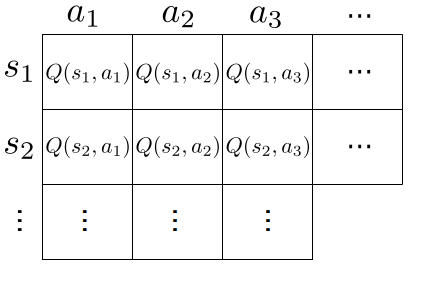
\includegraphics[width = 0.5\textwidth]{figures/figures_introduction/Q_table.pdf}
\caption{Example Q-table} 
\label{fig_chap1:Q_table}
\end{center}
\end{figure}
%

Q-learning is a tabular method for model-free RL~\cite{Watkins:1989a,Watkins:1992a,Clifton:2020a}.
%
The primary advantage of Q-learning compared to previous algorithms is the reduction in computational complexity of updating the policy during training.
%
Since the goal of RL is to iteratively optimize the policy, multiple versions of the policy must be evaluated. The value of being in each state will depend on the policy being used, such that a new policy would require the value function under that policy to be reevaluated for every state. Q-learning modifies how the value of a state is calculated, such that modifying the policy does not require recalculating the value function for every state, thus reducing the computational complexity of evaluating new policies. The action-value function represents the value of applying any action, $a$, at the current state, $s$, then following the policy, $\pi$, thereafter:
%
\begin{equation}
Q^\pi(s,a) = R(a)+\gamma\sum_{s'}P_{ss'}[\pi(s)]V^{\pi}(s')
\end{equation}
%
This is used to aggregate a Q-table that stores the evaluation of the action-value function for all combinations of states and actions, as illustrated in Figure~\ref{fig_chap1:Q_table}.
Q-learning allows the action-value function, $Q$, to approximate the optimal action-value function independently of the current policy.
% This allows the value of the current state and action to be evaluated without invalidating the value of the next state, $V^{\pi}(s')$.
This provides a way to incrementally update the existing Q-table without needing to regenerate a new table for every policy update.
%
% \rnotes{Edit and refine this. Add formula for updating Q-values. Find citations for other implementations/explanations.}
%
The success of Q-learning motivated the development of other algorithms that utilize action-value functions~\cite{Jang:2019a}.
%
However, because Q-learning is a tabular method, it suffers from the ``curse of dimensionality.'' The Q-learning algorithm has to experience every combination of state and action repeatedly. This is problematic for high dimensional problems such as multi-degree-of-freedom systems or multiple-input systems. This also makes it difficult to use for continuous problems since the system must be discretized to be solved by Q-learning. These challenges motivated the introduction of general function approximation methods to represent the value and action-value for any combination of state and action~\cite{Baird:1995a,Xu:2014a}.

\section{Deep Reinforcement Learning}
\label{sec:deep_RL_overview}
% \rnotes{Who was the first to try deep RL?}
Although tabular RL methods often work well for problems with discrete action and observation spaces, tabular methods are restrictive for high-dimensional problems since the size of the tables need to increase with the size of the action and observation spaces, which increase computational complexity to find optimal policies. This restriction also prevents tabular RL from being used for continuous action and observation spaces. 
% Using tabular methods is restrictive for reinforcement learning.
% It usually works just fine for small problems with discrete action spaces and observation spaces, but the tables would have to be very large for problems with more action and observation spaces~\pc.
This issue is solved by using nonlinear function approximators.
% Function approximation can be thought of as an instance of supervised learning~\pc.
Neural networks are commonly employed as nonlinear function approximators for machine learning and have been used extensively in supervised learning and unsupervised learning~\cite{Alloghani:2020a}. RL is referred to as deep RL when a deep neural network is used to approximate the value function or policy. Neural networks in deep RL are able to mitigate the ``curse of dimensionality'' by directly approximating the nonlinear value function.
%
Whereas tabular methods require every combination of observation and action to be visited, using a neural network to approximate the value function generates continuous estimates of the value. This eliminates the need to visit every observation and allows a continuous observation space to be used.
%
One of the first successful deep RL algorithms was used to train agents to play Atari games, where the agents were trained directly from pixel data. These agents trained using deep RL were often able to match or surpass human performance~\cite{Mnih:2015a,Shao:2019a}.
%
These contributions have enabled the development of other RL algorithms to train agents for other high-dimensional problems.

%
\begin{figure}[tb]
	\begin{center}
	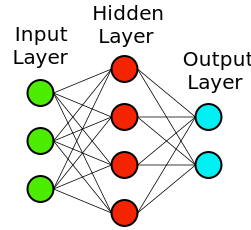
\includegraphics[width = 0.55\textwidth]{figures/figures_introduction/Neural_network_diagram.pdf}
	\caption{Neural network diagram} 
	\label{fig_chap1:NN_diagram}
	\end{center}
\end{figure}
%
An illustration of a neural network is shown in Figure~\ref{fig_chap1:NN_diagram}.
%
Neural networks are comprised of nodes which each have input and output signals.
%
Nodes of a neural network are arranged in layers. Nodes within each layer are not connected to each other, but each node is connected to nodes in the previous and following layer.
%
Each connection between the nodes is associated with a real-valued weight, and the value of the output signal from each node is computed from the value of the input signal and the weight of the connection.
%
The green nodes represent the input layer. In the case of RL, the input layer accepts the observations. The blue nodes represent the output layer. In RL, the outputs of the network can be the value in a state or the actions in the case of an actor-critic algorithm. The red nodes represent the hidden layers.
%
Although the number of nodes in the input and output layers are determined by the application, the number of hidden layers and the number of nodes in each hidden layer of deep neural networks can vary.
%
Networks with fewer nodes in the hidden layers have fewer parameters with which to approximate the value function. Increasing the size of the network generally allows the deep neural network to better approximate the value function due to having more parameters to adjust to get a good fit~\cite{Bengio:2009a}.
% This is what ``deep'' refers to in deep neural networks.
% \rnotes{and the activation function?}


% The sizes of the input and output layers of a neural network are determined by the application. For RL, the size of the input layer must match the number of observations and the size of the output layer must match the number of actions passed to the environment. The number of hidden layers and number of nodes in each hidden layer can vary.
% Deep neural networks with fewer nodes have fewer parameters with which to approximate the value function. Increasing the size of the network generally allows the deep neural network to better approximate the value function due to having more parameters to adjust to get a good fit~\cite{Bengio:2009a}.

% \rnotes{Discuss backpropagation for NN updates?}

There are many deep RL algorithms that have been developed. The main categories include value-based methods and actor critic methods. Noteworthy algorithms from these categories are described in the following sections.

% The return is the sum of the discounted future reward:
% \begin{equation}
% R=\sum_{t=0}^{t=\infty}=\gamma^t r(s_t,a_t
% \label{eq_chap1:reward_func}
% \end{equation}
% %
% where $\gamma$ is the discount factor and $r(s_t,a_t$ is the reward function.

% Value function:
% \begin{equation}
% V^\pi(s)
% \label{eq_chap1:value_func}
% \end{equation}

% Q-value function:
% \begin{equation}
% Q^\pi(s,a)
% \label{eq_chap1:Q-value_func}
% \end{equation}

\subsection{Value-Based Methods}
Value-based deep RL algorithms replace the tabular evaluation of the value or action-value function with a deep neural network capable of approximating continuous functions. This enables learning policies for systems with many observations or continuous observation spaces.
%
One of the first and most influential deep RL algorithms is the Deep Q-network (DQN) algorithm~\cite{Mnih:2013a,Mnih:2015a}.
DQN is based on the standard Q-learning algorithm with modifications that enable the use of deep neural networks to approximate the nonlinear action-value function.
%
% \rph{Linear function approximation methods had been used previously since training with nonlinear function approximators was unreliable.}
% DQN is based on the standard Q-learning algorithm, which is a tabular method, but includes a deep network to approximate the value function.
%
The use of deep neural networks allowed DQN to learn to play Atari games directly from raw pixel input. 
%
DQN produced performance comparable or superior to humans for four of the seven Atari games tested.
%
% \rnotes{DQN was shown to be able to learn to play Atari games directly from raw pixel input from an emulator. DQN produced performance comparable or superior to humans for four of the seven Atari games tested. It is an off-policy algorithm and does not require the network to be trained with data from the current policy. For off-policy algorithms, experience replay is used to store state-action samples from training into a replay buffer. A minibatch is sampled from the replay buffer for each network update phase. This improves data efficiency since past data can be used multiple times during training. This also reduces the correlation between samples used during each network update phase.}
%
Although DQN is able to operate on continuous observation spaces, it requires discrete action spaces since every action must be evaluated to find the optimal action from each state. This motivated the development of methods that can directly model the optimal policy.
% \rnotes{This is because DQN uses $\epsilon$-greedy policy?}

\subsection{Actor-Critic Methods}

%
\begin{figure}[tb]
\begin{center}
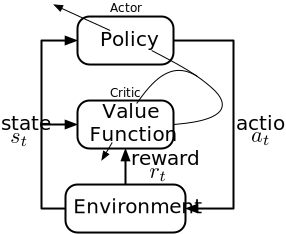
\includegraphics[width = 0.5\textwidth]{figures/figures_introduction/Actor_Critic_diagram.pdf}
\caption{Actor-critic diagram}
\label{fig_chap1:AC_diagram}
\end{center}
\end{figure}
%

% \rnotes{Prioritize explaining the specific equations used for actor critic methods.}
%
% \rph{The use of neural networks to approximate the value function allows continuous observation spaces to be used since every combination of states and actions do not need to be explored to determine its value. However, action spaces are still required to be discrete since every action must be tried to determine the optimal policy over a state-evolution. A function defining the actions to be used is necessary to provide a continuous action space.}
One method to directly learn policies is to model them using deep neural networks.
Using a function approximator such as a neural network to model the policy allows inputs from observations to produce actions in a continuous action space.
%
% Continuous action spaces can be achieved by using a neural network directly to approximate a policy.
One type of RL algorithm that takes advantage of neural networks to produce both continuous action spaces and continuous observation spaces is an actor-critic algorithm, where the value function and policy are modeled using separate neural networks~\cite{Lillicrap:2016a,Fujimoto:2018a}.
% Actor-critic algorithms don't rely on calculating an action based on the neural network parameterizing the value function.
% One network is used to learn the value function, another network is used to learn the policy.
A diagram illustrating the basic function of an actor-critic algorithm is shown in Figure~\ref{fig_chap1:AC_diagram}. The actor portion of the algorithm contains the policy and provides the action to the environment. The critic contains the network that approximates the value function. Both the actor and critic networks must be progressively updated to produce accurate estimates of the expected cumulative reward as well as the optimal policy that maximizes the reward.
% \rnotes{So, what are the limitations of DQN?}

% \rnotes{Generalized policy iteration may be important to know about here~\pc[Sutton and Barto 1998].}

%%%%%%%%%%%%%%%%%%%%%%%%%%%%%%%%%%%%%%%%%%%%%%%%%%%%%%%%%%%%%%%%%%%%%%%%%%%%%%%%%%%%%%%%%%

% \rph{The standard way to generate the policy from the approximation of the value or action-value is not useful for continuous action spaces modeled by neural networks, as in actor-critic. This is often achieved by using greedy maximization. This is fine for discrete, low-dimensional action spaces, but it is problematic for continuous action spaces since greedy maximization requires global maximization. It is more convenient to change the policy based on the gradient of the action-value network. This was first proposed by Sutton et al.~\cite{Sutton:1999a}. \what{This allows for the policy to be moved in the direction of optimal iteratively at each evaluation without having to perform optimization on every parameter at every evaluation?} Policy gradient improves reliability to converge towards locally optimal policies. \what{There was then work done to allow this to be done for deterministic policies~\cite{Silver:2014a}}. Policy updates rely on changing the parameters of the policy based on the gradient of the performance, i.e. the reward.} \rnotes{Get some of the equations from deterministic policy gradient, and explain in one or two sentences why it is advantageous over stochastic policy gradient.}

% The equations that are important for actor-critic algorithms are:

% Policy gradient:
% \begin{equation}
% \nabla_\theta J(\theta)\approx\mathbb{E}_{\tau}\sum_{t=0}^{T-1}\nabla_\theta \log \pi_\theta(a_t|s_t)A_{\pi_\theta}
% \label{eq_chap1:policy_gradient}
% \end{equation}
% %
% where $A_{\pi_\theta}$ is the advantage function. \rnotes{I think maybe for algorithms like DDPG and other Q function based algorithms, $G_t$ is replaced with the Q-value, $Q_t$}. The advantage function is:
% %
% \begin{equation}
% A_{\pi_\theta}(s_t,a_t)=r(s_t,a_t)+V_{\pi_\theta}(s_{t+1})-V_{\pi_\theta}(s_{t})
% \label{eq_chap1:advantage_func}
% \end{equation}
% %
% The policy parameters are updated by:
% %
% \begin{equation}
% \theta=\theta+\alpha\nabla_\pi J(\theta)
% \label{eq_chap1:actor_update}
% \end{equation}
% %
% and the critic parameters are updated by:
% %
% \begin{equation}
% \omega=\omega+\alpha\delta_t
% \label{eq_chap1:critic_update}
% \end{equation}
% %

%%%%%%%%%%%%%%%%%%%%%%%%%%%%%%%%%%%%%%%%%%%%%%%%%%%%%%%%%%%%%%%%%%%%%%%%%%%%%%%%%%%%%%%%%%

\subsection{Deep Deterministic Policy Gradient}
% \rnotes{Check this against DDPG and TD3. Find more detail on policy gradient and the one for value updates.}
% \rnotes{Should I make this less technical?}
A noteworthy development in actor-critic algorithms came from the development of the Deep Deterministic Policy Gradient (DDPG) algorithm~\cite{Lillicrap:2016a}.
% One of the algorithms used for this work is Deep Deterministic Policy Gradient (DDPG).DDPG is an actor-critic method that neural networks for both the actor and critic. This allows DDPG to be used for high-dimensional continuous state and action spaces.
The critic portion of DDPG is inspired by Deep Q Network (DQN)~\cite{Mnih:2013a,Mnih:2015a}. The actor portion of DDPG is updated based on the Deterministic Policy Gradient (DPG), which allows the policy to be updated based on the gradient of the value function~\cite{Silver:2014a}.

%%%%%%%%%%%%%%%%%%%%%%%%%%%%%%%%%%%%%%%%%%%%%%%%%%%%%%%%%%%%%%%%%%%%%%%%%%%%%%%%%%%%%%%%%%

% The policy gradient can be calculated by \rnotes{I think this is actually stochastic}:
% %
% \begin{equation}
% \nabla_{\theta^\mu}J\approx \frac{1}{N}\sum_i\nabla_aQ(s,a|\theta^Q)|_{s=s_i,a=\mu(s_i)}\nabla_{\theta^\mu}\mu(s|\theta^\mu)|s_i
% \end{equation}
% %
% The deterministic policy gradient is:
% %
% \begin{equation}
% \nabla_{\theta}J(\mu_\theta) = \mathbb{E}_{s\sim\rho^{\mu}} [\nabla_\theta\mu_\theta(s) \nabla_a Q^\mu(s,a)|_{a=\mu_\theta(s)}]
% \end{equation}
% %
% The policy parameters are updated by \rnotes{Is this right?}:
% %
% \begin{equation}
% \theta=\theta+\alpha\nabla_\pi J(\theta)
% \label{eq_chap1:actor_update}
% \end{equation}
% %
% The critic is updated by minimizing the loss as in Q-learning:
% %
% \begin{equation}
% L=\frac{1}{N}\sum_i(y_i-Q(s_i,a_i|\theta^Q))^2
% \end{equation}
% %
% where $y_i$ is the target value:
% %
% \begin{equation}
% y_i=r_i+\gamma Q'(s_{i+1},\mu'(s_{i+1}|\theta^{\mu'})|\theta^{Q^'})
% \end{equation}
% %
% \rph{This equation seems to basically be a correction for the Q-function using the current reward instead of the Q-value with the current state and action.
% It is apparently very important to have target networks, $Q'$ and $\mu'$, because you are trying to calculate the target value using, $y_i$, using $Q$, but $Q$ is also being updated. This makes $Q$ prone to divergence if target networks are not used~\cite{Mnih:2013a}.}

%%%%%%%%%%%%%%%%%%%%%%%%%%%%%%%%%%%%%%%%%%%%%%%%%%%%%%%%%%%%%%%%%%%%%%%%%%%%%%%%%%%%%%%%%%

\subsection{Twin-Delay DDPG}
A common disadvantage of deep RL algorithms is the occurrence of overestimation. This occurs when the algorithm overestimates the value approximation, often resulting in suboptimal policies. 
% \rph{Although DDPG provided a way to learn optimal policies for continuous observation and action spaces, this algorithm has a problem with overestimation. This overestimation is common for algorithms using function approximation and often leads to suboptimal policies.}
The Twin-Delay DDPG (TD3) algorithm is a modification of the DDPG algorithm that limits the occurrence of overestimation~\cite{Fujimoto:2018a}. This is accomplished by using two critic networks, where the policy is updated according to the critic with the lowest value estimate to avoid overly optimistic updates.
% Twin-Delay DDPG (TD3) uses a pair of critic networks to limit overestimation.
%
This makes the action-value estimates more accurate to more reliably find optimal policies.
% \rph{One critic network is updated frequently while the other is updated with a delay. This makes the action-value estimates more reliable since it is less susceptible to abrupt changes in the action-value.}

\section{Problems with RL}
\label{sec:RL_drawbacks}
%
Although RL has advantages over other methods for approximating optimal controllers, it also has drawbacks that have prevented its widespread adoption.
%
One of the primary drawbacks is the iteration needed to train policies, which often requires significant training time. This is illustrated by Figure~\ref{fig_chap1:long_training_time} showing reward during training. At the beginning of training, the policy performs poorly and produces low reward. This not only corresponds to a suboptimal policy but may also indicate that the policy causes unsafe behavior or does not perform the desired task, making it unusable. More training time is required before the policy achieves a suitable threshold of performance to allow it to be implemented for its intended purpose.

The tendency to perform poorly in the initial stage of training is a drawback that prevents training directly on physical systems. For instance, using a poorly performing policy on a robotic system may result in the system behaving in a way that causes it to damage itself or its surroundings.
The iteration required during training also reduces the feasibility of training on physical systems since this may require significant human supervision to reset the system for each iteration or if a failure occurs due to the poor performance. Training in simulation is faster and can be more easily automated to require less human supervision.
%
However, agents trained in simulation often have degraded performance when transferred to physical systems due to modeling error and sensor noise.
There has been a large amount of research performed to bridge the gap between simulation and physical applications, or sim-to-real~\cite{Peng2018a,Zhao:2020a}. This often requires initially training in simulation then completing training on the physical system.

%
\begin{figure}[tb]
\begin{center}
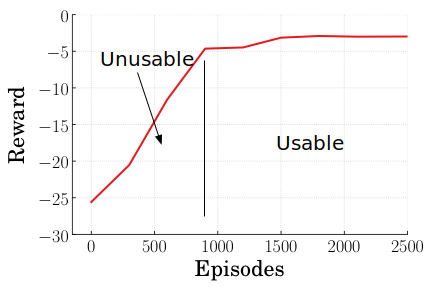
\includegraphics[width = 0.7\textwidth]{figures/figures_introduction/long_training_time}
\caption{Example of initial unusable policy} 
\label{fig_chap1:long_training_time}
\end{center}
\end{figure}
%

Another drawback to RL is the difficulty to develop performance guarantees for RL agents.
% \rph{It also tends to be difficult to develop performance guarantees for RL agents.}
In particular, the lack of stability guarantees prevents the adoption of RL in many applications.
Although some applications such as games do not require stability guarantees, physical applications, such as robotics and autonomous navigation, require stability guarantees in order to provide trust in the agent before implementation.
% \rnotes{In some cases we may want to guarantee stability over a certain operating region.} With standard RL algorithms, there is no way to guarantee how big the region of stability is. \rnotes{Post-hoc analysis after training runs into the standard difficulties for nonlinear systems.}
One method for training stable agents is to design a set of stabilizing controllers to serve as candidate controllers that the agent has to switch between~\cite{Perkins:2002a}. This method uses discrete actions to choose the appropriate stabilizing controller resulting in a discontinuous controller that is stable but suboptimal. Another method for learning stable agents involves providing an initial stabilizing policy and constraining any modification to the policy to remain stable~\cite{Berkenkamp:2017a}. As the agent learns, it is able to increase its approximated region of attraction. While this method provides safe and stabilizing agents within the region of attraction, it sacrifices exploration at the expense of stability. Additionally, a stabilizing initial policy must be provided. It is beneficial to have agents that achieve stability without having to pre-design stable policies for the RL controllers.

% \rnotes{Some work has tried to use different ways to parameterize RL to ensure stability~\cite{Friedrich:2017a}. I didn't completely understand those methods.}

RL agents also tend to be difficult to interpret, particularly deep RL agents. Because of the large number of nodes in a deep neural network required to model the policy, it is difficult to intuitively understand the control law learned by the agent, making the agent a black box~\cite{Alharin:2020a}. As with the inability to generate stability guarantees, this prevents the adoption of RL for many applications since it is difficult to predict the behavior of the agents in a wide range of scenarios. Some methods used to interpret agents require manual summarization of the behavior of the agent~\cite{Amir:2019a,Lage:2019a}. Other methods utilize decision trees, illustrated in Figure~\ref{fig_chap1:decision_tree}, which can help interpretability by reducing the complexity of the deep model into a concise graphical model~\cite{Bastani:2018a}.
%
Decision trees often require training a shallow model from a deep neural network model. However, agents with continuous action spaces or those that learn complex behaviors may require large decision trees that are still difficult to interpret.
%
% \what{Decision trees require training a shallow model from a deep neural network model. However, complex deep networks often require large decision trees, reducing the interpretability of the model~\pc.}

%
\begin{figure}[tb]
\begin{center}
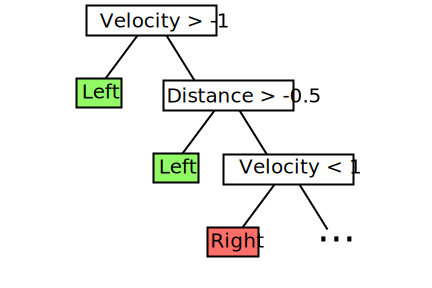
\includegraphics[width = 0.6\textwidth]{figures/figures_introduction/Decision_tree.pdf}
\caption{Example of a decision tree}
\label{fig_chap1:decision_tree}
\end{center}
\end{figure}
%

\section{Combining RL and Conventional Control}
\label{sec:combined_control_overview}

Although RL agents can learn policies without knowledge of the model of the system being controlled, a model is often available for use by the control systems designer. This is always the case for agents that are initially trained in simulation. Additionally, if a system model is known, an experienced controls engineer will also often have knowledge of how to design a controller that enables the system to accomplish the desired goal even if the controller is suboptimal.
%
RL controllers can be trained in a way to take advantage of established domain knowledge of dynamics and control theory. This can include direct design of controllers that combine RL and conventional control elements that both contribute to the total system input~\cite{Eaglin:2020a,Eaglin:2023a}. Domain knowledge may also be used indirectly through the design of the environment, such as reward function design. Domain knowledge can also be utilized in the analysis of agent performance after training to improve interpretability and generate performance guarantees. 

The following chapters present contributions that the combination of RL and conventional control have to the control design processes:
% Contributions of this work include:
\begin{itemize}
	\item Chapter~\ref{chapter2} introduces multiple controller architectures for combining RL with conventional control. The baseline performance of these combined controllers applied to multiple benchmark systems is then presented. The combined controllers are shown to generally reduce required training time to generate acceptable policies. Design guidelines are then presented based on the performance of the controllers.
	\item Chapter~\ref{chapter3} presents stability evaluations of the combined controllers.
	% Methods to design agents to satisfy certain stability conditions are also presented.
	\item Chapter~\ref{chapter4} presents the effects of the combined controllers on robustness to modeling error.
	\item Chapter~\ref{chapter5} proposes a method to use domain knowledge to improve interpretability of the learned controllers by approximating the agent with a piecewise set of control laws.
	\item Chapter~\ref{chapter6} presents an analysis of the current commercializability of this work.
\end{itemize}

% \begin{itemize}
% 	\item RL can be done model-free
% 	\item It does not require any knowledge of how to design control systems to train an agent
% 	\item But we often do have some idea how to design a control system for something
% 	\item We can use domain knowledge of dynamics and control to solve the problems listed above
% 	\item Combination of RL with domain knowledge can include
% 	\begin{itemize}
% 		\item Building a model/domain-knowledge-based controller directly to learn alongside the agent
% 		\item Informed design of other parts of the environment (like stability-based reward function)
% 		\item Post-hoc analysis and interpretation based on more properly understood methods
% 	\end{itemize}
% \end{itemize}

% \section{Contributions}

% {\color{red}The following chapters propose various methods used to plan trajectories for flexible mobile robots while limiting vibration. These include methods to limit vibration in trajectory tracking problems as well as planning paths which induce low vibration. While most work treats path planning and vibration control sequentially, these algorithms provide concurrent path planning and vibration control by incorporating explicit vibration constraints in the path planning algorithms.}

%
% \begin{table}[tb]
% \begin{center}
% \setlength{\tabcolsep}{15pt}
% \caption{Combined Controller ($K_{p}=5$) 5\% Settling Times}
% \vspace{-2ex}
% \begin{tabular}{l c c}
% \toprule
% \textbf{Step} & \textbf{5\% Settling Times (\si{\second})} & \textbf{Normalized}\\
% \midrule
% % $0$--$25$\si{\micro\meter} & \num{0.0017751}\\
% % $25$--$50$\si{\micro\meter} & \num{0.0017549}\\
% % $50$--$75$\si{\micro\meter} & \num{0.001446}\\
% % $75$--$100$\si{\micro\meter} & \num{0.0011047}\\
% $0$--$0.025$\si{\milli\meter} & \num{0.00178} & 0.88\\
% $0.025$--$0.5$\si{\milli\meter} & \num{0.00175} & 0.86\\
% $0.05$--$0.075$\si{\milli\meter} & \num{0.00145} & 1.99\\
% $0.075$--$0.1$\si{\milli\meter} & \num{0.00110} & 0.57\\
% \bottomrule
% \label{table:Combined_res_ch_Kp5}
% \end{tabular}
% \end{center}
% % \end{table}
% % %
% \vspace{-3ex}
% % \begin{table}[tb]
% \begin{center}
% \setlength{\tabcolsep}{15pt}
% \caption{Combined Controller ($K_{p}=10$) 5\% Settling Times}
% % \vspace{-1ex}
% \begin{tabular}{l c c}
% \toprule
% \textbf{Step} & \textbf{5\% Settling Times (\si{\second})} & \textbf{Normalized} \\
% \midrule
% % $0$--$25$\si{\micro\meter}  & \num{0.0011929}\\
% % $25$--$50$\si{\micro\meter}  & \num{0.0006639}\\
% % $50$--$75$\si{\micro\meter} & \num{0.0007425}\\
% % $75$--$100$\si{\micro\meter}  & \num{0.0007227}\\
% $0$--$0.025$\si{\milli\meter} & \num{0.00119} & 0.59\\
% $0.025$--$0.5$\si{\milli\meter} & \num{0.000664} & 0.33\\
% $0.05$--$0.075$\si{\milli\meter} & \num{0.000743} & 1.02\\
% $0.075$--$0.1$\si{\milli\meter} & \num{0.000723} & 0.37\\
% \bottomrule
% \label{table:Combined_res_ch_Kp10}
% \end{tabular}
% \end{center}
% \end{table}
% %


% \begin{figure}[tb]
% \begin{center}
% 	\begin{minipage}{0.45\textwidth}
% 	\begin{center}
% 	\includegraphics[width = \columnwidth]{figures/Chapter1_fig/Actuator_PID_with_shaping_Kp5_current}
% 	\caption{Current input for $K_{p}=5$}
% 	\label{fig:Actuator_PID_with_shaping_Kp5_current}
% 	\end{center}
% 	\end{minipage}
% \hspace{0.07\textwidth}
% 	\begin{minipage}{0.45\textwidth}
% 	\begin{center}
% 	\includegraphics[width = \columnwidth]{figures/Chapter1_fig/Actuator_PID_with_shaping_Kp10_current}
% 	\caption{Current input for $K_{p}=10$}
% 	\label{fig:Actuator_PID_with_shaping_Kp10_current}
% 	\end{center}
% 	\end{minipage}
% \end{center}
% \vspace{-0.2in}
% \end{figure}


% \begin{enumerate}
% 	\item \textbf{Development of an open-loop trajectory tracking method to minimize the tracking error of a flexible system} -- Chapter \ref{chapter2}
% 		\begin{itemize}	
% 			\item[] An open-loop vibration control method for trajectory tracking is presented. Trajectory tracking error resulting from vibration was minimized for arbitrary, pre-planned trajectories.
% 		\end{itemize}
% 	\item \textbf{Development of a discrete motion planner using vibration optimal movements} -- Chapter \ref{chapter3}
% 		\begin{itemize}
% 			\item [] An existing discrete path planner was adapted to plan paths that produce low-vibration. The new path planner generates trajectories such that vibration canceling pulses can be used to track the trajectory.
% 			% The planner utilizes movements which cancel vibration.
% 			This method is compared to input shaping to analyze time optimality.
% 		\end{itemize}
% 	\item \textbf{Development of an optimal sampling-based motion planner to produce continuous low-vibration trajectories} -- Chapter \ref{chapter4}
% 		\begin{itemize}
% 			\item[] A probabilistically complete sampling-based path planner which produces continuous trajectories for a flexible system is presented. Trajectories are planned while respecting kinematic and actuator constraints. A local planner is also presented to solve the two-point boundary value problem for flexible systems.
% 		\end{itemize}
% \end{enumerate}

% The next chapter will introduce a trajectory tracking method to minimize tracking error of systems following preplanned paths. Chapter \ref{chapter3} then introduces a discrete planning algorithm to generate paths that can be followed using a sequence of predefined optimal commands. This method generates trajectories that can be tracked with zero error. In Chapter \ref{chapter4}, a sampling-based algorithm modified from RRT and RRT* is discussed. This method generates low cost trajectories while accounting for actuator limits and velocity constraints. Chapter \ref{chapter5} then presents conclusions and potential future work.








% \begin{table}[t!]
% \centering
% \caption{Impulse Amplitudes and Spacing for Two Input Shaper}
% \label{table:multi-impulses}
% \begin{tabular}{@{}rrrr@{}}
% \toprule
% \multicolumn{1}{l}{} &  & \multicolumn{2}{c}{Impulse Amplitudes} \\ \midrule
% Impulse Times &  & Input $f_1$ & Input $f_2$ \\ \cmidrule(l){3-4} 
% 0 &  & 0.50 & 0.07 \\
% 0.84 &  & 0.09 & 0.94 \\
% 1.69 &  & 0.41 & 0.00 \\ \bottomrule
% \end{tabular}
% \end{table}

%%%%%%%%%%%%%%%%
% Chapter 2
%%%%%%%%%%%%%%%%

%!TEX root = thesis.tex

\chapter{Reinforcement Learning Control with Model-Based Elements}
\label{chapter2}

Although Reinforcement Learning (RL) can be implemented model-free, where an agent is trained without domain knowledge of control systems, it is common for the practitioner to have experience with dynamics and control.
For systems for which a model is known, there is often some understanding of how to design a controller to accomplish the desired task, especially for linear systems or systems that can be approximated as linear. For instance, PID and LQR are well documented linear control methods that can be applied to many problems.
% \rph{provided nonlinearity is negligible.}
%
Even though a controller may be found to accomplish the goal, such as remaining stable near a reference trajectory, optimal controllers cannot generally be found analytically for nonlinear systems. This challenge can be solved with RL, which is capable of iteratively generating optimal controllers for cases which cannot be solved analytically. However, it is often time-consuming to train RL agents due to the iteration required. Additionally, initial policies often perform poorly.
%

Controllers that combine conventional control methods with RL can
address the drawbacks of both methods by allowing RL to be of benefit where it is most needed.
% \rph{The impact of inefficient RL training algorithms can be overcome for cases in which there is domain knowledge about the dynamics of the system or how to design controllers that provide suboptimal but satisfactory controllers.}
% For cases in which a satisfactory controller can be designed, RL does not have to learn ``\rph{from scratch}.''
%
% \rph{Combined controllers reduce the exploration needed for the agent to find a desirable optimal policy.}
% RL can be used in conjunction with controllers designed using domain knowledge of conventional control methods to reduce the exploration needed for the agent to find a desirable optimal policy. 
% This allows RL to be of benefit where it is most needed.
Instead of using RL to learn what is already understood by the designer, it can be used to extend beyond the domain knowledge of the designer.
%
The way in which this domain knowledge should be utilized depends on the system being controlled and the desired goal of the controller. The following section introduces classification categories for different control structures for this combined control approach that have been investigated in this work. The performance of these control structures is then described, followed by a summary of the performance and
guidelines for designing combined controllers for a variety of systems.

\section{Control Structures}
\label{sec_chap2:control_structure}

% \subsection{RL-Alone}
\subsection{Pure RL}
Controllers utilizing an RL agent alone are used as a baseline for evaluating the effects of various combined controller architectures. 
% \rph{This uses the standard format for training as was illustrated by Figure~\ref{fig_chap1:AC_diagram}.}
%
The implementation of the trained agent is represented by the block diagram in Figure~\ref{fig_chap2:pure_RL_block_diagram}, where $\boldsymbol{s}_d$ is the desired state, $u$ is the agent output, and $\boldsymbol{s}$ is the current state of the plant. Since the agent controller is acting on its own without any contribution from any model-based controller, the input to the plant is the agent action, $u=a_t$.
%
\begin{figure}[tb]
\begin{center}
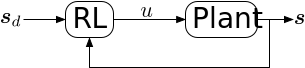
\includegraphics[width = 0.5\textwidth]{figures/figures_RL_model_based_control/Block_diagram_RL_alone.pdf}
\caption{Block diagram for Pure RL control structure} 
\label{fig_chap2:pure_RL_block_diagram}
\end{center}
\end{figure}
%

\subsection{RL and Fixed-Gain Control}
%
\begin{figure}[tb]
    \begin{center}
    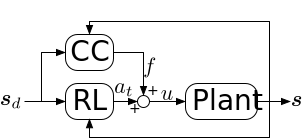
\includegraphics[width = 0.5\textwidth]{figures/figures_RL_model_based_control/Block_diagram_combined_control.pdf}
    \caption{Block diagram for RL and fixed-gain control structure} 
    \label{fig_chap2:fixed_gain_block_diagram}
    \end{center}
    \end{figure}
    %
    \begin{figure}[tb]
    \begin{center}
    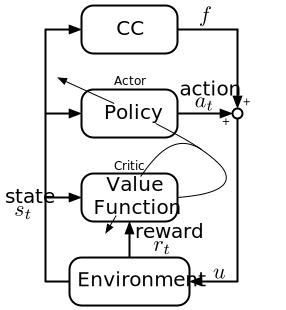
\includegraphics[width = 0.5\textwidth]{figures/figures_RL_model_based_control/Actor_Critic_diagram_fixed_gain.pdf}
    \caption{Learning diagram for RL with fixed-gain control} 
    \label{fig_chap2:fixed_gain_actor_critic}
    \end{center}
    \end{figure}
    %
One proposed control architecture for combining domain knowledge with RL uses fixed-gain control components in parallel with the learned policy. The block diagram for this control architecture is shown in Figure~\ref{fig_chap2:fixed_gain_block_diagram}, where the CC block represents Conventional Control, or a model-based controller designed using domain knowledge of dynamics and control. The plant input, $u$, for this control structure is:
%
\begin{equation}
u=f(\boldsymbol{s}) + a_t
\label{eq_chap2:fixed_RL_block_diagram}
\end{equation}
%
where $f(\boldsymbol{s})$ is a fixed-gain input that is a function of the state, $\boldsymbol{s}$.
The specific design of $f(\boldsymbol{s})$ depends on the system and goal of the controller.
%
For instance, it could be designed such that it could function on its own to provide satisfactory (though suboptimal) performance, or it can be designed to perform well for only a subset of the desired operation space for the system.

The RL component of the controller will still need to interact with the fixed-gain component and modify the controller output to optimize the combined control policy. This provides the designer with the ability to design a simple controller that can provide satisfactory performance while leaving the more difficult optimal control problem to be solved by the RL agent.
%
The training process for this type of controller is illustrated by a modified actor-critic training diagram in Figure~\ref{fig_chap2:fixed_gain_actor_critic}. The action output from the policy, $a_t$, is combined with the output from the conventional controller, $f$. The sum of the outputs, $u$, is the input to the environment.
% The output from the conventional controller and action from the policy combine to become the input for the environment.
However, the value function only evaluates the action, $a_t$, not the total input to the environment. Since the value function and policy are unaffected by the conventional control block, the addition of the fixed-gain term is equivalent to changing the environment.

\subsection{Agent-Driven Gain Scheduling}
%
\begin{figure}[tb]
\begin{center}
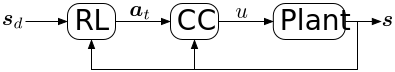
\includegraphics[width = 0.7\textwidth]{figures/figures_RL_model_based_control/Block_diagram_cont_gain_sched_control.pdf}
\caption{Block diagram for RL continuous gain-scheduling control structure} 
\label{fig_chap2:cont_gain_sched_block_diagram}
\end{center}
\end{figure}
%

In the fixed-gain and RL controller architecture, the agent is unable to modify the component of the controller designed using domain knowledge.
In addition to this controller architecture,
% using a fixed-gain controller in parallel with RL to take advantage of domain knowledge,
the combined controller can be designed to have the agent interact directly with the domain-knowledge controller. One way to realize this direct interaction is by using a gain-scheduled controller for which the agent learns the scheduling law. This is shown by the block diagram in Figure~\ref{fig_chap2:cont_gain_sched_block_diagram}, where the controller output, $u$, is:
% One of the control structures combining RL and controls domain knowledge is a agent-driven gain scheduling type of controller shown in the block diagram in Figure~\ref{fig_chap2:cont_gain_sched_block_diagram}.
% It can also be combined with a model-based fixed-gain term such that the plant input, $u$ from the controller is:
%
\begin{equation}
u = \boldsymbol{a}_t\boldsymbol{s}
\label{eq_chap2:cont_gain_sched_RL_block_diagram}
\end{equation}
%
and $\boldsymbol{a}_t$ is a vector of the agent outputs, $\boldsymbol{a}_t=[a_t^{(1)}, \, a_t^{(2)}, \, \dots, \, a_t^{(n)}]$, corresponding to a feedback controller with $n$ states.
Implementation of the agent as a gain scheduling mechanism allows for domain knowledge to be used to design the feedback controller.
It may also improve interpretability, since the response at each time step can be understood as a system subject to a linear feedback controller.
%
Figure~\ref{fig_chap2:gain_sched_actor_critic} shows the learning process for the gain-scheduled RL controller.
%
The set of actions, $a_t$, is a set of gains that are used to update the gain-scheduled feedback controller in the CC block. The output, $u$, from the controller is passed to the environment and causes its state, $s_t$, to change. The reward is used to update the value function so that the gain update law can be optimized. This controller architecture provides a more integrated combination between the parts of the controller designed using domain knowledge and the parts learned by RL.
%
\begin{figure}[tb]
    \begin{center}
    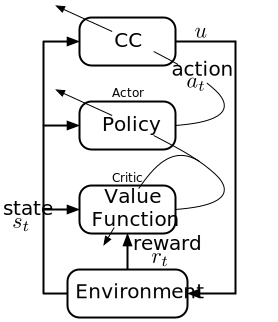
\includegraphics[width = 0.5\textwidth]{figures/figures_RL_model_based_control/Actor_Critic_diagram_gain_sched.pdf}
    \caption{Learning diagram for RL with gain scheduled control} 
    \label{fig_chap2:gain_sched_actor_critic}
    \end{center}
\end{figure}
%

Training RL agents requires selecting training parameters such as the RL algorithm, neural network architecture, and episode length. The training parameters were tuned for each benchmark problem and will be introduced for each system alongside each set of results. Additional information about the mechanical parameters for each benchmark system and the hyperparameters used for training are found in Appendix A.

\section{Duffing Oscillator Benchmark System}
\label{sec_chap2:Duffing_oscillator}
\subsection{Problem Description}

%
\begin{figure}[t]
\begin{center}
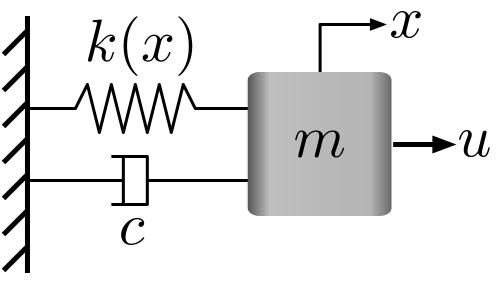
\includegraphics[width = 0.5\textwidth]{figures/figures_RL_model_based_control/Duffing_oscillator.pdf}
\caption{Duffing oscillator model}
\label{fig_chap2:duffing_model}
\end{center}
\end{figure}
% 
A duffing oscillator model was used as a simple benchmark model to illustrate the usefulness of combined RL and conventional control methods. The model is shown in Figure~\ref{fig_chap2:duffing_model}, where $m$ is the mass, $c$ is the damping coefficient, $x$ is the displacement, $k(x)$ is the nonlinear spring stiffness, and $u$ is the force input. The equation of motion for this system is:
%
\begin{equation}
m\ddot{x} + c\dot{x} + k(x)x = u
\label{eq_chap_2:duffing_EOM}
\end{equation}
%
where the nonlinear stiffness is
$k(x)=\alpha + \beta x^2$.
% $k(x)=\alpha + 3\beta x^2$.
The displacement is constrained between $-1.5\si{\meter}\leq x \leq 1.5\si{\meter}$. The desired behavior of the system is to move the mass from rest at $x=0$ to a desired displacement, $x_d$, while limiting oscillation amplitude. The reward function used to accomplish this was:
%
\begin{equation}
    r = -(x_d - x)^2
    \label{eq_chap2:duffing_reward_function}
\end{equation}
%
Although this reward function is simple, it accomplishes the desired task by requiring the position error to be quickly minimized in order to maximize reward.

The previously described combined control structures were applied to the duffing oscillator. The Pure RL controller uses a force output as the action applied to the system. For the combined controllers, a fixed-gain component was designed to provide a constant force that stabilizes the system about the desired displacement, $x_d$. The force which stabilizes the system at the desired equilibrium is:
%
\begin{equation}
f(\boldsymbol{s})=\alpha x_d + \beta x^3_d
\label{eq_chap_2:feedforward}
\end{equation}
%
% \rnotes{For the case with the fixed feedforward term alone (FF), the input allows the system to oscillate about the setpoint. Because of this, the controllers which combine the feedforward term and an agent in parallel, RL-LA and RL-PD, cause the system to nearly reach the setpoint. For these controllers, the model-based feedforward term is responsible for causing the system to perform the desired task of reaching the setpoint while the agent modifies the force input to reduce ISE.}
The response of the duffing oscillator with this fixed-gain controller and desired displacement of $x_d=1$ is shown in Figure~\ref{fig:duffing_feedforward}. Although the fixed-gain controller causes the system to move to the desired displacement, the settling time is high. In the combined controllers, the RL components are responsible for modifying the fixed-gain component to optimize the response.
%
\begin{figure}[tb]
    \centering
      % \vspace{-5ex}
      % \includegraphics[width=\columnwidth]{figures/RL_RL-PD_RL-LA_500steps}
      % \includegraphics[width=3in]{figures/RL_RL-PD_RL-LA_500steps}
      \includegraphics[width=0.65\columnwidth]{figures/figures_RL_model_based_control/time_responses_duffing/duffing_FF/Displacement_1_init_0_steps}
      \vspace{-2ex}
      \caption{Duffing oscillator response with fixed-gain term}
      % \vspace{-2ex}
      \label{fig:duffing_feedforward}
\end{figure}
%
This fixed-gain controller was used for two combined controllers, one that uses a single scalar action and another that uses a gain-scheduled controller. In summary, the set of controllers tested on the duffing oscillator are:
%
\begin{align}
    &\qquad\qquad\text{Pure RL:} & u&=a_t \qquad\qquad\qquad\\
    &\qquad\qquad\text{RL-PD:} & u&=\alpha x_d + \beta x_d^3 - a_t^{(1)}(x-x_d) - a_t^{(2)} \dot{x}\\
    &\qquad\qquad\text{RL-LA:} & u&=\alpha x_d + \beta x_d^3 + a_t \qquad\qquad\qquad
\end{align}
%
Pure RL is the baseline controller that uses the action, $a_t$, from RL as the only input to the system. RL-PD uses the fixed-gain controller in \eqref{eq_chap_2:feedforward} in addition to a Proportional-Derivative (PD) controller, where the actions $a_t^{(1)}$ and $a_t^{(2)}$ are gains for the displacement error and velocity of the system. RL-Lumped Action (RL-LA) uses the fixed-gain controller with a lumped action, or single scalar action. 

\subsection{Baseline Performance}
%
\begin{figure}[tb]
    \centering
      % \vspace{-5ex}
      % \includegraphics[width=\columnwidth]{figures/Duffing_ISE_while_training_shaded}
      % \includegraphics[width=3in]{figures/Duffing_ISE_while_training_shaded}
      \includegraphics[width=0.65\columnwidth]{figures/figures_RL_model_based_control/duffing_mean_reward_v_episode}
      \vspace{-2ex}
      \caption{Mean duffing oscillator reward during training}
      % \vspace{-2ex}
      \label{fig_chap2:duffing_reward_trend}
    \end{figure}
    %

The agents for each controller were trained using the Twin Delayed DDPG (TD3) algorithm~\cite{Fujimoto:2018a}.
%
All neural networks had two hidden layers, containing $400$ and $300$ nodes, respectively, and used the rectified linear unit (RELU) activation function as was used in the original TD3 paper. The observations included measurements of the displacement, $x$, and velocity, $\dot{x}$, of the mass, analogous to full-state feedback for a conventional controller, as well as the desired displacement, $x_d$.
%
Training was conducted over $40$ episodes.
% which is $80$ episodes at a $50\si{\hertz}$ sampling rate.
The desired displacement was randomized at the initialization of each episode.
% For each episode, a random setpoint is generated based on an initial seed.
Since RL relies on stochasticity, five agents were trained for each control structure. The same set of five initial seeds was used for the different control structures.
% After training was completed, a new trial begins with a new initial seed, and the agent is reinitialized. The same set of random seeds is used for each method. Fifteen trials were performed for each method.
%
After training the agents, they were tested to compare the performance of the controllers without model-based components to those with model-based and RL components.

%
The performance of the agents during training was evaluated at fixed intervals using the reward received from the system starting at rest with a desired displacement of $x_d=1\si{\meter}$.
The reward trends during training are shown in Figure~\ref{fig_chap2:duffing_reward_trend}, where the lines are the mean reward, and the shaded regions are standard deviation for the five agents of each controller type. The Pure RL controllers begin training with the lowest reward whereas the RL-PD controllers begin with the highest reward. Although the reward from the RL and RL-LA controllers tend to increase after the beginning of training, the reward from RL-PD initially significantly decreases. This is due to one of the responses becoming unstable, which skews the mean and standard deviation. The mean rewards from the different controllers converge to approximately the same value after 20 episodes.
%

Time responses from the agents at the beginning of training are shown in Figure~\ref{fig_chap2:duffing_0_steps}.
%
The low reward at the beginning of training with Pure RL was caused by one of the responses being unstable and the steady-state error from the other responses resulting from the inability of the controller to force the system to reach the desired displacement, $x_d$, as shown in Figure~\ref{subfig_chap2:duffing_pure_RL_0_steps}.
%
\begin{figure}[tb]
    \centering
    \begin{subfigure}[b]{0.49\textwidth}
        \centering
        \includegraphics[width=\textwidth]{figures/figures_RL_model_based_control/time_responses_duffing/duffing_pure_RL/Displacement_1_init_0_steps.pdf}
        \caption{Pure RL}
        \label{subfig_chap2:duffing_pure_RL_0_steps}
    \end{subfigure}\\
    \hfill
    \begin{subfigure}[b]{0.49\textwidth}
        \centering
        \includegraphics[width=\textwidth]{figures/figures_RL_model_based_control/time_responses_duffing/duffing_RL_PD/Displacement_1_init_0_steps.pdf}
        \caption{RL-PD}
        \label{subfig_chap2:duffing_RL_PD_0_steps}
    \end{subfigure}
    \hfill
    \begin{subfigure}[b]{0.49\textwidth}
        \centering
        \includegraphics[width=\textwidth]{figures/figures_RL_model_based_control/time_responses_duffing/duffing_RL_LA/Displacement_1_init_0_steps.pdf}
        \caption{RL-LA}
        \label{subfig_chap2:duffing_RL_LA_0_steps}
    \end{subfigure}
    \hfill
    \caption{Duffing oscillator responses before training}
    \label{fig_chap2:duffing_0_steps}
\end{figure}
%
% When using Pure RL, without a feedforward term, the agent does not cause the system to reach the desired setpoint.
%
Since the combined controllers have the fixed-gain component, \eqref{eq_chap_2:feedforward}, they cause the system to move near the desired displacement. The responses with RL-PD in Figure~\ref{subfig_chap2:duffing_RL_PD_0_steps} do not have overshoot and tend to have shorter settling times than the other controllers. Since the controller output of the gain-scheduled PD component is zero at the desired displacement, the combination of the fixed-gain component and PD component in RL-PD results in zero steady-state error. Similar to RL-PD, the RL-LA responses in Figure~\ref{subfig_chap2:duffing_RL_LA_0_steps} settle near the desired displacement. However, the responses have higher oscillation amplitude and some responses have steady-state error. These responses show that the combined controllers have better performance than the Pure RL controller even before training.
%

%
\begin{figure}[tb]
    \centering
    \begin{subfigure}[b]{0.49\textwidth}
        \centering
        \includegraphics[width=\textwidth]{figures/figures_RL_model_based_control/time_responses_duffing/duffing_pure_RL/Displacement_1_init_10000_steps.pdf}
        \caption{Pure RL}
        \label{subfig_chap2:duffing_pure_RL_10000_steps}
    \end{subfigure}\\
    \hfill
    \begin{subfigure}[b]{0.49\textwidth}
        \centering
        \includegraphics[width=\textwidth]{figures/figures_RL_model_based_control/time_responses_duffing/duffing_RL_PD/Displacement_1_init_10000_steps.pdf}
        \caption{RL-PD}
        \label{subfig_chap2:duffing_RL_PD_10000_steps}
    \end{subfigure}
    \hfill
    \begin{subfigure}[b]{0.49\textwidth}
        \centering
        \includegraphics[width=\textwidth]{figures/figures_RL_model_based_control/time_responses_duffing/duffing_RL_LA/Displacement_1_init_10000_steps.pdf}
        \caption{RL-LA}
        \label{subfig_chap2:duffing_RL_LA_10000_steps}
    \end{subfigure}
    \hfill
    \caption{Duffing oscillator responses after training}
    \label{fig_chap2:duffing_10000_steps}
\end{figure}
%
Time responses of the duffing oscillator after the agent controllers were trained are shown in Figure~\ref{fig_chap2:duffing_10000_steps}. The responses with Pure RL in Figure~\ref{subfig_chap2:duffing_pure_RL_10000_steps} settled near the desired displacement at $x_d=1\si{\meter}$ with low oscillation amplitude. However, all of the responses have steady-state error. The RL-PD responses in Figure~\ref{subfig_chap2:duffing_RL_PD_10000_steps} have zero steady-state error just as the responses before training. However, one response has overshoot and another response has a long rise time. The RL-LA responses in Figure~\ref{subfig_chap2:duffing_RL_LA_10000_steps} have short rise times; however, they have steady-state error and two of the responses have long settling times due to oscillation. The response characteristics of the Pure RL and combined controllers are summarized in Table~\ref{table:duffing_resp_char}. The RL-PD controllers had the best performance in all categories. Pure RL has higher mean steady-state error than RL-LA, however, RL-LA has much longer settling time and higher overshoot.
%
\begin{table}[tb]
    \begin{center}
      \setlength{\tabcolsep}{6pt}
      \caption{Duffing Oscillator Response Characteristics}
      \begin{tabular}{ l c c c c}
      \hline\hline
       & & Settling Time & Steady-state Error & Percent Overshoot \\
      \hline
      \multirow{2}{*}{\textbf{RL}} & \text{Mean} & 2.212\si{\second} & 0.064\si{\meter} & 6.047\%\\
       & \text{SD} & 2.885\si{\second} & 0.025\si{\meter} & 7.702\% \\
      \hline
      \multirow{2}{*}{\textbf{RL-PD}} & \text{Mean} & \textbf{1.372}\si{\second} & \textbf{0.0}\si{\meter} & \textbf{0.5}\%\\
       & \text{SD} & \textbf{0.598}\si{\second} & \textbf{0.0}\si{\meter} & \textbf{1.174}\%\\
      \hline
      \multirow{2}{*}{\textbf{RL-LA}} & \text{Mean} & 14.62\si{\second} & 0.0587\si{\meter} & 11.839\%\\
       & \text{SD} & 18.672\si{\second} & 0.0283\si{\meter} & 15.004\%\\
      \label{table:duffing_resp_char}
      \end{tabular}
      % \vspace{-0.2in}
    \end{center}
\end{table}
%

Although the Pure RL controller was not designed with any domain knowledge, it still provides good performance after training. RL-PD had the best performance overall. Its controller architecture also relied more heavily on domain knowledge since it included both a fixed-gain component and a state-feedback control component for which the agents only had to learn appropriate parameters. The responses from the RL-LA controllers have slightly lower steady-state error than the Pure RL controllers due to the fixed-gain component; however, settling times for RL-LA were inconsistent.
% more training would be required to get more consistent settling times. \dots

% \rnotes{Comment out overshoot and settling time plots during training.}
% \begin{figure}[tb]
% \centering
%   % \vspace{-5ex}
%   % \includegraphics[width=\columnwidth]{figures/RL_RL-PD_RL-LA_2500steps}
%   \includegraphics[width=0.65\columnwidth]{figures/figures_RL_model_based_control/RL_RL-PD_RL-LA_trial1_2500steps}
%   \vspace{-2ex}
%   \caption{Response at 2500 training steps}
%   % \vspace{-2ex}
%   \label{fig:Response_2500steps}
% \end{figure}
% %
% %
% \begin{figure}[tb]
% \centering
%   % \vspace{-5ex}
%   % \includegraphics[width=\columnwidth]{figures/RL_RL-PD_RL-LA_10000steps}
%   % \includegraphics[width=3in]{figures/RL_RL-PD_RL-LA_10000steps}
%   \includegraphics[width=0.65\columnwidth]{figures/figures_RL_model_based_control/RL_RL-PD_RL-LA_trial1_5000steps}
%   \vspace{-2ex}
%   \caption{Response at 5000 training steps}
%   % \vspace{-2ex}
%   \label{fig:Response_5000steps}
% \end{figure}
% %

% Although the reward used to train the agents is analogous to ISE, other performance metrics were also used to compare the performance of the combined feedforward and RL controllers to the controller using Pure RL. The mean $5\%$ settling times from the controllers during training are shown in Figure \ref{fig:Settingwhiletraining}. Due to the way settling time was measured, a settling time of $5\si{\second}$ in the figure corresponds to a true settling time of $5\si{\second}$ or longer.
% %
% The settling time with Pure RL remained above that of RL-PD and RL-LA throughout training. Although the settling time of RL-PD does not show a clear trend, the settling time for RL-LA tends to decrease as training progresses. The high settling times during training with RL and at the beginning of training with RL-LA primarily result from steady-state error, where the system settles at a position below the desired setpoint.

% The mean percent overshoot from the controllers, shown in Figure \ref{fig:Overshootwhiletraining}, was also used to evaluate the controllers. It follows a similar trend as was shown in the time response plots, where the overshoot from Pure RL at the beginning of training tends to be lower than that from RL-PD and RL-LA due to the system not reaching the desired setpoint. Although, the mean overshoot for the three methods are similar near the end of training, the mean maximum overshoot of Pure RL is significantly higher than that of the other methods.

% %
% \begin{figure}[tb]
% \centering
%   % \vspace{-5ex}
%   % \includegraphics[width=\columnwidth]{figures/Duffing_settling_while_training_shaded}
%   % \includegraphics[width=3in]{figures/Duffing_settling_while_training_shaded}
%   \includegraphics[width=0.65\columnwidth]{figures/figures_RL_model_based_control/Duffing_settling_while_training_mean}
%   \vspace{-2ex}
%   \caption{Mean settling time while training}
%   % \vspace{-2ex}
%   \label{fig:Settingwhiletraining}
% \end{figure}
% %
% \begin{figure}[tb]
% \centering
%   % \vspace{-5ex}
%   % \includegraphics[width=\columnwidth]{figures/Duffing_overshoot_while_training_shaded}
%   % \includegraphics[width=3in]{figures/Duffing_overshoot_while_training_shaded}
%   \includegraphics[width=0.65\columnwidth]{figures/figures_RL_model_based_control/Duffing_overshoot_while_training_mean}
%   \vspace{-2ex}
%   \caption{Mean percent overshoot while training}
%   % \vspace{-2ex}
%   \label{fig:Overshootwhiletraining}
% \end{figure}
% %

\section{Double-Pendulum Crane}
\subsection{Problem Description}
%
\begin{figure}[tb]
\begin{center}
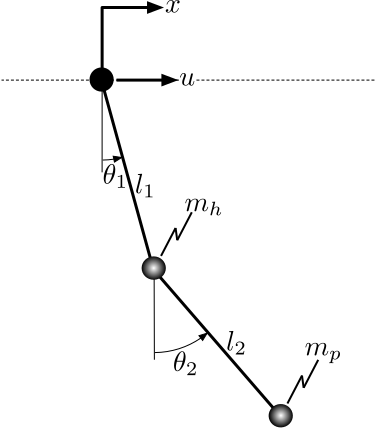
\includegraphics[width = 0.44\textwidth]{figures/figures_RL_model_based_control/Double_pendulum_crane_model.pdf}
\caption{Double-pendulum planar crane model}
\label{fig_chap2:planar_crane}
\end{center}
\end{figure}
%

A planar double-pendulum crane, shown by the model in Figure~\ref{fig_chap2:planar_crane}, was used as a second benchmark system for the combined RL controllers.
The double-pendulum crane is a three degree-of-freedom underactuated system.
This model approximates the dynamics of physical cranes where a payload is fastened to the crane by a hook with non-negligible mass. The payload is manipulated by moving a crane trolley on a horizontal track.
The displacement of the trolley along the track is described by $x$. The angular displacements of the hook and payload pendulums are $\theta_1$ and $\theta_2$, respectively, both measured from the vertical axis of the Newtonian frame. The lengths of the pendulums, commonly called hoist length and rigging length, are $l_1$ and $l_2$. The hook mass is $m_h$, and the payload mass is $m_p$. The input, $u$, is desired acceleration of the trolley. The goal of the controllers for this system was to move the trolley to a desired displacement while minimizing oscillation of the pendulums.
% \rph{Direct acceleration control was used as the system input, $u$.}
%
The equations of motion for the double-pendulum crane are:
%
% \begin{equation}
% \begin{multline}
% \dot{x},\\
% \dot{\theta_1},\\
% \dot{\theta_2},\\
% u_t,\\
% (-L_1*L2*mp*(sin(\theta_1)*sin(\theta_2) + cos(\theta_1)*cos(\theta_2))*(-L_1*L2*mp*(-sin(\theta_1)*cos(\theta_2) + sin(\theta_2)*cos(\theta_1))*\dot{\theta}_1^2 - L_1*L2*mp*(sin(\theta_1)*sin(\theta_2) + cos(\theta_1)*cos(\theta_2))*(-L_1*L2*mp*(sin(\theta_1)*cos(\theta_2) - sin(\theta_2)*cos(\theta_1))*\dot{\theta_2}^2 - L_1*g*mh*sin(\theta_1) - L_1*g*mp*sin(\theta_1))/(L_1^2*mh + L_1^2*mp) - L2*g*mp*sin(\theta_2) - (-L_1*L2*mp*(sin(\theta_1)*sin(\theta_2) + cos(\theta_1)*cos(\theta_2))*(L_1*mh*cos(\theta_1) + L_1*mp*cos(\theta_1))/(L_1^2*mh + L_1^2*mp) + L2*mp*cos(\theta_2))*acceleration_command)/(-L_1^2*L2^2*mp^2*(sin(\theta_1)*sin(\theta_2) + cos(\theta_1)*cos(\theta_2))^2/(L_1^2*mh + L_1^2*mp) + L2^2*mp) - L_1*L2*mp*(sin(\theta_1)*cos(\theta_2) - sin(\theta_2)*cos(\theta_1))*\dot{\theta_2}^2 - L_1*g*mh*sin(\theta_1) - L_1*g*mp*sin(\theta_1) - (L_1*mh*cos(\theta_1) + L_1*mp*cos(\theta_1))*acceleration_command)/(L_1^2*mh + L_1^2*mp),\\
% (-L_1*L2*mp*(-sin(\theta_1)*cos(\theta_2) + sin(\theta_2)*cos(\theta_1))*\dot{\theta_1}^2 - L_1*L2*mp*(sin(\theta_1)*sin(\theta_2) + cos(\theta_1)*cos(\theta_2))*(-L_1*L2*mp*(sin(\theta_1)*cos(\theta_2) - sin(\theta_2)*cos(\theta_1))*\dot{\theta_2}^2 - L_1*g*mh*sin(\theta_1) - L_1*g*mp*sin(\theta_1))/(L_1^2*mh + L_1^2*mp) - L2*g*mp*sin(\theta_2) - (-L_1*L2*mp*(sin(\theta_1)*sin(\theta_2) + cos(\theta_1)*cos(\theta_2))*(L_1*mh*cos(\theta_1) + L_1*mp*cos(\theta_1))/(L_1^2*mh + L_1^2*mp) + L2*mp*cos(\theta_2))*acceleration_command)/(-L_1^2*L2^2*mp^2*(sin(\theta_1)*sin(\theta_2) + cos(\theta_1)*cos(\theta_2))^2/(L_1^2*mh + L_1^2*mp) + L2^2*mp)
% \end{multline}
% \end{equation}
%
\begin{multline}
\left [
\begin{array}{ccc}
1 & 0 & 0\\
l_1\cos(\theta_1)(m_h + m_p) & l_1^2(m_h + m_p) & l_1l_2m_p\cos(\theta_1-\theta_2)\\
l_2m_p\cos(\theta_2) & l_1l_2m_p\cos{(\theta_1-\theta_2)} & l_2^2m_p\\
\end{array}
\right ]
\left [
\begin{array}{c}
\ddot{x}\\
\ddot{\theta}_1\\
\ddot{\theta}_2
\end{array}
\right ] \\
=
\left [
\begin{array}{c}
u\\
-l_1l_2m_p\sin(\theta_1-\theta_2)\dot{\theta}_2^2 - l_1g\sin(\theta_1)(m_h + m_p)\\
-l_1l_2m_p\sin(\theta_2-\theta_1)\dot{\theta}_1^2 - l_2gm_p\sin(\theta_2)\\
\end{array}
\right ]
\end{multline}
%
The acceleration of the crane trolley, $\ddot{x}$, is determined by only the control output, $u$. The dynamics of the pendulums are coupled with each other and the acceleration of the trolley.
%
The incremental reward function for this system is:
%
\begin{equation}
r = -\omega_xx^2 - \omega_{\theta_1}\theta_1^2 - \omega_{\theta_2}\theta_2^2
\label{eq_chap2:reward_crane}
\end{equation}
%
where $\omega_x$, $\omega_{\theta_1}$, and $\omega_{\theta_2}$ are weights designed to normalize the reward terms to have approximately equal importance during training.

%
\begin{figure}[tb]
    \centering
    \begin{subfigure}[b]{0.49\textwidth}
        \centering
        \includegraphics[width=\textwidth]{figures/figures_RL_model_based_control/time_responses_crane/dpcrane_fixed_gain/Cart_displacement_0p185_init_300000_steps.pdf}
        \caption{Trolley displacement response}
        \label{subfig_chap2:dpcrane_fixed_gain_trolley_resp}
    \end{subfigure}\\
    \hfill
    \begin{subfigure}[b]{0.49\textwidth}
        \centering
        \includegraphics[width=\textwidth]{figures/figures_RL_model_based_control/time_responses_crane/dpcrane_fixed_gain/Hook_displacement_0p185_init_300000_steps.pdf}
        \caption{Hook displacement response}
        \label{subfig_chap2:dpcrane_fixed_gain_hook_resp}
    \end{subfigure}
    \hfill
    \begin{subfigure}[b]{0.49\textwidth}
        \centering
        \includegraphics[width=\textwidth]{figures/figures_RL_model_based_control/time_responses_crane/dpcrane_fixed_gain/Payload_displacement_0p185_init_300000_steps.pdf}
        \caption{Payload displacement response}
        \label{subfig_chap2:dpcrane_fixed_gain_payload_resp}
    \end{subfigure}
    \hfill
    \caption{Crane responses from fixed-gain term}
    \label{fig_chap2:dpcrane_fixed_gain_resp}
\end{figure}
%

The Pure RL, fixed-gain and RL, and gain-scheduled RL control elements were applied to this system. The fixed-gain term, $f(\boldsymbol{s})=k_p x + k_d \dot{x}$, is a PD controller, where the gains, $k_p$ and $k_d$, are designed to move the trolley to the desired displacement without input saturation and with a damping coefficient of $\zeta=\frac{\sqrt{2}}{2}$.
%
Time responses of the crane subject to the fixed-gain controller are shown in Figure~\ref{fig_chap2:dpcrane_fixed_gain_resp}. This movement excites unwanted oscillation in the pendulums, shown in Figure~\ref{subfig_chap2:dpcrane_fixed_gain_hook_resp} and Figure~\ref{subfig_chap2:dpcrane_fixed_gain_payload_resp}. Since the fixed-gain controller does not account for motion of the pendulums, the agent must modify the control output to limit hook and payload oscillation.
%

Multiple combined controllers consisting of fixed-gain, gain-scheduled, and lumped action terms were tested on the benchmark double-pendulum crane.
%
While the fixed-gain term only accounts for the trolley position and velocity, the gain scheduling term only accounts for pendulum motion. Because of this, one combined controller uses the fixed-gain control element combined with the gain-scheduled control element. Another combined controller uses the fixed-gain terms with a lumped action term learned by the agent.
Additionally, a controller combining the features of all the above controllers was tested, where the control output is determined by a fixed-gain, gain-scheduled, and lumped-action control elements. In summary, the control laws for the crane are:
%
\begin{align}
&\qquad\qquad\text{Pure RL:} & u&=a_t \qquad\qquad\qquad\\
&\qquad\qquad\text{RL-PD:} & u&=k_px+k_d\dot{x} + \boldsymbol{a}_t\boldsymbol{\theta} \qquad\qquad\qquad\\
&\qquad\qquad\text{RL-LA:} & u&=k_px+k_d\dot{x} + a_t \qquad\qquad\qquad\\
&\qquad\qquad\text{RL-PD-LA:} & u&=k_px+k_d\dot{x} + \boldsymbol{a}_t\boldsymbol{\theta} + a_t \qquad\qquad\qquad
\end{align}
%
where Pure RL is the baseline RL controller that does not utilize any domain knowledge. RL-PD is the controller with the fixed-gain term combined with a gain-scheduled term, where $\boldsymbol{a}_t$ are gains assigned by the agent and are updated at every time step, and $\boldsymbol{\theta}$ are the states describing the motion of the pendulums. RL-Lumped-Action (RL-LA) uses the fixed-gain control element with a single (lumped) action from the agent. RL-PD-LA combines fixed-gain, gain-scheduled, and lumped action control elements.
% where $\boldsymbol{a}_t$ are the agent assigned gains for the pendulum states and $\boldsymbol{\theta}$ is the vector of angular states. \rnotes{Maybe I could use a different symbol.}

\subsection{Baseline Performance}
%
\begin{figure}[tb]
        \centering
        \includegraphics[width=0.65\columnwidth]{figures/figures_RL_model_based_control/dpcrane_mean_reward_v_episode.pdf}
        \vspace{-2ex}
        \caption{Mean crane reward during training for $x(0)=0.185\si{\meter}$}
      % \vspace{-2ex}
        \label{fig:dpcrane_mean_reward_baseline}
\end{figure}
%
The TD3 algorithm~\cite{Fujimoto:2018a} was used to train five agents for each controller using Pure RL, RL-PD, RL-LA, and RL-PD-LA. The same set of five initial seeds was used for the different controllers. Each episode during training was initialized with the crane at rest with a trolley displacement of $x(0)=0.185\si{\meter}$ and hook and payload angular displacements of $\theta_1=\theta_2=0$. The desired final displacement of the trolley was $x(t_f)=0\si{\meter}$. Trends during training are shown to evaluate the baseline performance of the controller types. Figure \ref{fig:dpcrane_mean_reward_baseline} shows the mean reward earned from the five trained agents of each controller type. The shaded region shows the standard deviation of the rewards at each sampled episode of training. The untrained performance of the combined controllers at 0 episodes is better than that of the controller using Pure RL. However, near the end of training, at 3000 episodes, the rewards earned by each controller are approximately equal.
%

The higher initial reward from the combined controllers is due to the fixed-gain term commanding the trolley to move to the desired location, whereas more training is necessary for the agent of the Pure RL controller to learn to move the trolley to the desired location.
%
This can be seen by isolating the contribution of the trolley response to the total reward, where the reward contribution from the trolley is:
%
\begin{equation}
    r_{x} = -\omega_x x^2
\end{equation}
%
The reward from the trolley is shown in Figure~\ref{fig:mean_settling_baseline}.
%
Although the combined controllers start with higher reward from the trolley displacement, the agents for the Pure RL controller learn to increase the trolley reward after training for only a short time. The trolley reward for RL-LA tends to be the highest for the controllers tested.
%
\begin{figure}[tb]
    \centering
    % \includegraphics[width=\columnwidth]{figures/Mean_settling_v_episode.pdf}
    \includegraphics[width=0.65\columnwidth]{figures/figures_RL_model_based_control/Trolley_reward_v_episode.pdf}
    \vspace{-2ex}
    % \caption{Mean settling time during training}
    \caption{Mean reward from trolley during training}
  % \vspace{-2ex}
    \label{fig:mean_settling_baseline}
\end{figure}
  %

Figure~\ref{fig_chap2:dpcrane_trolley_resp_0steps} shows the trolley displacement responses for the different controllers before training.
% where the neural network parameters of the agents are randomly initialized.
The crane begins at rest with initial trolley displacement of $x(0)=0.185\si{\meter}$ and pendulum displacements $\theta_1=\theta_2=0$.
The trolley responses for Pure RL do not settle near the equilibrium and instead diverge towards the limits of the workspace, as shown in Figure~\ref{subfig_chap2:dpcrane_trolley_resp_0steps_pure_RL}. The responses for RL-PD in Figure~\ref{subfig_chap2:dpcrane_trolley_resp_0steps_gain_sched} have the best trolley performance, where most of the responses converge near the desired displacement with low oscillation amplitude due to the fixed-gain terms. The RL-LA responses in Figure~\ref{subfig_chap2:dpcrane_trolley_resp_0steps_RL_LA} have higher error in trolley displacement than RL-PD but have lower oscillation amplitude. The RL-PD-LA responses in Figure~\ref{subfig_chap2:dpcrane_trolley_resp_0steps_RL_PD_LA} have less trolley displacement error than RL-LA, but some of the responses have high oscillation amplitude.
%
\begin{figure}[tb]
    \centering
    \begin{subfigure}[b]{0.49\textwidth}
        \centering
        \includegraphics[width=\textwidth]{figures/figures_RL_model_based_control/time_responses_crane/dpcrane_pure_RL/Cart_displacement_0p185_init_0_steps.pdf}
        \caption{Pure RL}
        \label{subfig_chap2:dpcrane_trolley_resp_0steps_pure_RL}
    \end{subfigure}
    \hfill
    \begin{subfigure}[b]{0.49\textwidth}
	    \centering
	    \includegraphics[width=\textwidth]{figures/figures_RL_model_based_control/time_responses_crane/dpcrane_cont_gain_sched/Cart_displacement_0p185_init_0_steps.pdf}
	    \caption{RL-PD}
	    \label{subfig_chap2:dpcrane_trolley_resp_0steps_gain_sched}
    \end{subfigure}
    \hfill
    \begin{subfigure}[b]{0.49\textwidth}
        \centering
        \includegraphics[width=\textwidth]{figures/figures_RL_model_based_control/time_responses_crane/dpcrane_RL_LA/Cart_displacement_0p185_init_0_steps.pdf}
        \caption{RL-LA}
        \label{subfig_chap2:dpcrane_trolley_resp_0steps_RL_LA}
    \end{subfigure}
    \hfill
    \begin{subfigure}[b]{0.49\textwidth}
        \centering
        \includegraphics[width=\textwidth]{figures/figures_RL_model_based_control/time_responses_crane/dpcrane_RL_PD_LA/Cart_displacement_0p185_init_0_steps.pdf}
        \caption{RL-PD-LA}
        \label{subfig_chap2:dpcrane_trolley_resp_0steps_RL_PD_LA}
    \end{subfigure}
    \hfill
    \caption{Crane trolley responses for $x(0)=0.185\si{\meter}$ before training}
    \label{fig_chap2:dpcrane_trolley_resp_0steps}
\end{figure}
%

Figure~\ref{fig_chap2:dpcrane_trolley_resp_300000steps} shows the trolley displacement responses for the different controllers after training, where the crane begins at rest with initial trolley displacement of $x(0)=0.185\si{\meter}$ and pendulum displacements $\theta_1=\theta_2=0$.
Three of the five Pure RL agents shown in Figure~\ref{subfig_chap2:dpcrane_trolley_resp_300000steps_pure_RL} can bring the trolley to the desired displacement within the allotted time, whereas two responses do not converge to zero displacement. The RL-PD responses in Figure~\ref{subfig_chap2:dpcrane_trolley_resp_300000steps_gain_sched} tend to have higher oscillation amplitude than the other controllers. Figure~\ref{subfig_chap2:dpcrane_trolley_resp_300000steps_RL_LA} shows that the RL-LA responses tend to be able to converge closer to zero displacement than Pure RL. The RL-PD-LA responses in Figure~\ref{subfig_chap2:dpcrane_trolley_resp_300000steps_RL_PD_LA} are also able to converge to be close to the desired displacement at $x(t_f)=0\si{\meter}$, but exhibit some oscillation.
%
\begin{figure}[tb]
    \centering
    \begin{subfigure}[b]{0.49\textwidth}
        \centering
        \includegraphics[width=\textwidth]{figures/figures_RL_model_based_control/time_responses_crane/dpcrane_pure_RL/Cart_displacement_0p185_init_300000_steps.pdf}
        \caption{Pure RL}
        \label{subfig_chap2:dpcrane_trolley_resp_300000steps_pure_RL}
    \end{subfigure}
    \hfill
    \begin{subfigure}[b]{0.49\textwidth}
	    \centering
	    \includegraphics[width=\textwidth]{figures/figures_RL_model_based_control/time_responses_crane/dpcrane_cont_gain_sched/Cart_displacement_0p185_init_300000_steps.pdf}
	    \caption{RL-PD}
	    \label{subfig_chap2:dpcrane_trolley_resp_300000steps_gain_sched}
    \end{subfigure}
    \hfill
    \begin{subfigure}[b]{0.49\textwidth}
        \centering
        \includegraphics[width=\textwidth]{figures/figures_RL_model_based_control/time_responses_crane/dpcrane_RL_LA/Cart_displacement_0p185_init_300000_steps.pdf}
        \caption{RL-LA}
        \label{subfig_chap2:dpcrane_trolley_resp_300000steps_RL_LA}
    \end{subfigure}
    \hfill
    \begin{subfigure}[b]{0.49\textwidth}
        \centering
        \includegraphics[width=\textwidth]{figures/figures_RL_model_based_control/time_responses_crane/dpcrane_RL_PD_LA/Cart_displacement_0p185_init_300000_steps.pdf}
        \caption{RL-PD-LA}
        \label{subfig_chap2:dpcrane_trolley_resp_300000steps_RL_PD_LA}
    \end{subfigure}
    \hfill
    \caption{Crane trolley responses for $x(0)=0.185\si{\meter}$ after training}
    \label{fig_chap2:dpcrane_trolley_resp_300000steps}
\end{figure}
%
In both the cases before training and after training, the controllers utilizing a continuous gain scheduled term, RL-PD and RL-PD-LA, tend to exhibit oscillation near the desired displacement, whereas the controllers using a lumped action, Pure RL and RL-LA, have much lower oscillation amplitude. For the responses after training, the controllers that include a fixed-gain term and a lumped action, RL-LA and RL-PD-LA, tend to converge closer to the desired equilibrium and have lower steady state-error.
%
The response characteristics of the trolley are summarized in Table~\ref{table:dpcrane_trolley_resp_char}. RL-LA has the lowest values for all of the performance metrics shown. Although RL-PD has lower steady-state error and overshoot than Pure RL, it has higher residual oscillation amplitude. RL-PD-LA has lower steady-state error than Pure RL, but has higher values for residual oscillation amplitude and overshoot. In general, the combined controllers tend to have better performance than Pure RL for steady-state error and percent overshoot. However, RL-PD and RL-PD-LA have higher residual oscillation amplitudes due to the gain scheduling terms on the pendulum states.
%
\begin{table}[tb]
    \begin{center}
      \setlength{\tabcolsep}{6pt}
      \caption{Trolley Response Characteristics for $x(0)=0.185\si{\meter}$}
      \begin{tabular}{ l c c c c}
      \hline\hline
       & & Amplitude & Steady-state Error & Percent Overshoot \\
      \hline
      \multirow{2}{*}{\textbf{RL}} & \text{Mean} & 0.0005\si{\meter} & 0.027\si{\meter} & 24.8\%\\
       & \text{SD} & 0.0007\si{\meter} & 0.025\si{\meter} & 18.5\% \\
      \hline
      \multirow{2}{*}{\textbf{RL-PD}} & \text{Mean} & 0.004\si{\meter} & 0.024\si{\meter} & 21.6\%\\
       & \text{SD} & 0.003\si{\meter} & 0.017\si{\meter} & 17.4\%\\
      \hline
      \multirow{2}{*}{\textbf{RL-LA}} & \text{Mean} & \textbf{0.0}\si{\meter} & \textbf{0.02}\si{\meter} & \textbf{13.9}\%\\
       & \text{SD} & \textbf{0.0}\si{\meter} & \textbf{0.014}\si{\meter} & \textbf{5.9}\%\\
      \hline
      \multirow{2}{*}{\textbf{RL-PD-LA}} & \text{Mean} & 0.007\si{\meter} & 0.024\si{\meter} & 28.2\%\\
       & \text{SD} & 0.01\si{\meter} & 0.029\si{\meter} & 34\%\\
      \label{table:dpcrane_trolley_resp_char}
      \end{tabular}
      % \vspace{-0.2in}
    \end{center}
\end{table}
%

%
\begin{figure}[tb]
    \centering
    % \includegraphics[width=\columnwidth]{figures/Mean_swing_ISE_v_episode.pdf}
    \includegraphics[width=0.65\columnwidth]{figures/figures_RL_model_based_control/Swing_reward_v_episode.pdf}
    \vspace{-2ex}
    % \caption{Mean ISE of hook and payload swing during training}
    \caption{Mean reward from hook and payload during training}
  % \vspace{-2ex}
    \label{fig:mean_swing_ISE_baseline}
\end{figure}
%
% The mean reward shown in Figure~\ref{fig:dpcrane_mean_reward_baseline} also showed that RL-LA began training with the highest overall reward.
%
The previous evaluation of the contribution of the trolley responses to the reward is not adequate to understand the performance of the agents. Therefore, the reward contribution from the pendulum responses also needs to be analyzed.
% Since the contribution of the trolley response to total reward was analyzed in the previous paragraphs, the contribution of the pendulum responses needs to be analyzed as well.
% \rph{Since the fixed-gain term of the combined controllers was shown to provide similar trolley rewards, the difference in overall reward at training initialization is due to pendulum oscillation.}
The reward contribution from the oscillation of the hook and payload is:
%
\begin{equation}
    r_{\theta_1,\theta_2}=-\omega_{\theta_1} \theta_1^2 - \omega_{\theta_2} \theta_2^2
\end{equation}
%
The reward trends from the pendulum contributions are shown in Figure~\ref{fig:mean_swing_ISE_baseline}.
%
At the initialization of training, Pure RL begins with the highest reward followed by RL-LA with a slightly lower reward. The RL-PD and RL-PD-LA controllers have the lowest swing angle reward.
%
%
\begin{figure}[tb]
    \centering
    \begin{subfigure}[b]{0.49\textwidth}
        \centering
        \includegraphics[width=\textwidth]{figures/figures_RL_model_based_control/time_responses_crane/dpcrane_pure_RL/Payload_displacement_0p185_init_0_steps.pdf}
        \caption{Pure RL}
        \label{subfig_chap2:dpcrane_payload_resp_0steps_pure_RL}
    \end{subfigure}
    \hfill
    \begin{subfigure}[b]{0.49\textwidth}
	    \centering
	    \includegraphics[width=\textwidth]{figures/figures_RL_model_based_control/time_responses_crane/dpcrane_cont_gain_sched/Payload_displacement_0p185_init_0_steps.pdf}
	    \caption{RL-PD}
	    \label{subfig_chap2:dpcrane_payload_resp_0steps_gain_sched}
    \end{subfigure}
    \hfill
    \begin{subfigure}[b]{0.49\textwidth}
        \centering
        \includegraphics[width=\textwidth]{figures/figures_RL_model_based_control/time_responses_crane/dpcrane_RL_LA/Payload_displacement_0p185_init_0_steps.pdf}
        \caption{RL-LA}
        \label{subfig_chap2:dpcrane_payload_resp_0steps_RL_LA}
    \end{subfigure}
    \hfill
    \begin{subfigure}[b]{0.49\textwidth}
        \centering
        \includegraphics[width=\textwidth]{figures/figures_RL_model_based_control/time_responses_crane/dpcrane_RL_PD_LA/Payload_displacement_0p185_init_0_steps.pdf}
        \caption{RL-PD-LA}
        \label{subfig_chap2:dpcrane_payload_resp_0steps_RL_PD_LA}
    \end{subfigure}
    \hfill
    \caption{Crane payload responses for $x(0)=0.185\si{\meter}$ before training}
    \label{fig_chap2:dpcrane_payload_resp_0steps}
\end{figure}
%
The time responses of the payload before training are shown in Figure~\ref{fig_chap2:dpcrane_payload_resp_0steps}. The crane began at rest with an initial trolley displacement of $x(0)=0.185\si{\meter}$. The responses with Pure RL in Figure~\ref{subfig_chap2:dpcrane_payload_resp_0steps_pure_RL} and RL-LA in Figure~\ref{subfig_chap2:dpcrane_payload_resp_0steps_RL_LA} have relatively low oscillation amplitude. The RL-PD responses in Figure~\ref{subfig_chap2:dpcrane_payload_resp_0steps_gain_sched} and RL-PD-LA responses in Figure~\ref{subfig_chap2:dpcrane_payload_resp_0steps_RL_PD_LA} have higher amplitude oscillation, with some responses increasing amplitude with time. This corresponds with what was seen for the trolley responses at the start of training, where the controllers using agent-driven gain scheduling tended to have higher oscillation amplitude.

Figure~\ref{fig_chap2:dpcrane_payload_resp_300000steps} shows the time responses of the payload after training has been completed. The controllers that include a single lumped action term tend to have lower oscillation amplitude. This can be seen for Pure RL in Figure~\ref{subfig_chap2:dpcrane_payload_resp_300000steps_pure_RL}, RL-LA in Figure~\ref{subfig_chap2:dpcrane_payload_resp_300000steps_RL_LA} and RL-PD-LA in Figure~\ref{subfig_chap2:dpcrane_payload_resp_300000steps_RL_PD_LA}. RL-LA has the lowest oscillation amplitude, whereas RL-PD in Figure~\ref{subfig_chap2:dpcrane_payload_resp_300000steps_gain_sched} has the highest oscillation amplitude. This is consistent with the previous figures showing that the controllers that include a gain scheduling term tend to have higher oscillation amplitude. This is summarized in Table~\ref{table:dpcrane_payload_resp_char}, where RL-LA had the lowest mean residual oscillation amplitude. Although the mean oscillation amplitude for RL-PD-LA is the second highest, this was primarily due to one response skewing the mean.
%
\begin{figure}[tb]
    \centering
    \begin{subfigure}[b]{0.49\textwidth}
        \centering
        \includegraphics[width=\textwidth]{figures/figures_RL_model_based_control/time_responses_crane/dpcrane_pure_RL/Payload_displacement_0p185_init_300000_steps.pdf}
        \caption{Pure RL}
        \label{subfig_chap2:dpcrane_payload_resp_300000steps_pure_RL}
    \end{subfigure}
    \hfill
    \begin{subfigure}[b]{0.49\textwidth}
	    \centering
	    \includegraphics[width=\textwidth]{figures/figures_RL_model_based_control/time_responses_crane/dpcrane_cont_gain_sched/Payload_displacement_0p185_init_300000_steps.pdf}
	    \caption{RL-PD}
	    \label{subfig_chap2:dpcrane_payload_resp_300000steps_gain_sched}
    \end{subfigure}
    \hfill
    \begin{subfigure}[b]{0.49\textwidth}
        \centering
        \includegraphics[width=\textwidth]{figures/figures_RL_model_based_control/time_responses_crane/dpcrane_RL_LA/Payload_displacement_0p185_init_300000_steps.pdf}
        \caption{RL-LA}
        \label{subfig_chap2:dpcrane_payload_resp_300000steps_RL_LA}
    \end{subfigure}
    \hfill
    \begin{subfigure}[b]{0.49\textwidth}
        \centering
        \includegraphics[width=\textwidth]{figures/figures_RL_model_based_control/time_responses_crane/dpcrane_RL_PD_LA/Payload_displacement_0p185_init_300000_steps.pdf}
        \caption{RL-PD-LA}
        \label{subfig_chap2:dpcrane_payload_resp_300000steps_RL_PD_LA}
    \end{subfigure}
    \hfill
    \caption{Crane payload responses for $x(0)=0.185\si{\meter}$ after training}
    \label{fig_chap2:dpcrane_payload_resp_300000steps}
\end{figure}
%
%
\begin{table}[tb]
    \begin{center}
      \setlength{\tabcolsep}{6pt}
      \caption{Payload Residual Amplitude for $x(0)=0.185\si{\meter}$}
      \begin{tabular}{ l c c }
      \hline\hline
       & & Amplitude \\
      \hline
      \multirow{2}{*}{\textbf{RL}} & \text{Mean} & 0.474$^\circ$ \\
       & \text{SD} & 0.481$^\circ$ \\
      \hline
      \multirow{2}{*}{\textbf{RL-PD}} & \text{Mean} & 0.896$^\circ$ \\
       & \text{SD} & 0.23$^\circ$ \\
      \hline
      \multirow{2}{*}{\textbf{RL-LA}} & \text{Mean} & \textbf{0.015}$^\circ$ \\
       & \text{SD} & \textbf{0.03}$^\circ$ \\
      \hline
      \multirow{2}{*}{\textbf{RL-PD-LA}} & \text{Mean} & 0.756$^\circ$\\
       & \text{SD} & 0.947$^\circ$ \\
      \label{table:dpcrane_payload_resp_char}
      \end{tabular}
      % \vspace{-0.2in}
    \end{center}
\end{table}

The RL-LA controllers and RL-PD-LA controllers have the best overall performance in terms of limiting steady-state error and oscillation amplitude. They both tend to have lower trolley displacement error, where RL-PD-LA has lower error than RL-LA. However, RL-PD-LA achieves lower trolley steady-state error at the expense of higher pendulum oscillation. The Pure RL controllers tend to have the most trolley steady-state error since they do not have the benefit of the fixed-gain term to move the trolley towards zero displacement.

The results for the double-pendulum crane shown above were acquired from responses with initial trolley displacements equal to the one used for training. The fixed initial displacement of $x(0)=0.185\si{\meter}$ during training caused the agents to have the most experience for trolley displacements $0\leq x\leq 0.185\si{\meter}$. To show how the agents perform for initial displacements other than the one used for training, the following results show how the agents that were trained with an initial displacement of $x(0)=0.185\si{\meter}$ perform for an initial trolley displacement of $x(0)=-0.185\si{\meter}$ instead.
%
The reward trends from this initial trolley displacement are shown in Figure~\ref{fig:dpcrane_neg_mean_reward_baseline}. The initial rewards at the beginning of training are similar to those for initial displacements of $x(0)=0.185\si{\meter}$ in Figure~\ref{fig:dpcrane_mean_reward_baseline}. The fixed-gain terms cause the rewards from the combined controllers to begin higher than that of Pure RL. However, while the performance of the Pure RL controllers showed improvement from the initial reward, the other controllers do not show clear trends in improved performance.

%
\begin{figure}[tb]
    \centering
    \includegraphics[width=0.65\columnwidth]{figures/figures_RL_model_based_control/dpcrane_neg_mean_reward_v_episode.pdf}
    \vspace{-2ex}
    \caption{Mean crane reward during training for $x(0)=-0.185\si{\meter}$}
  % \vspace{-2ex}
    \label{fig:dpcrane_neg_mean_reward_baseline}
\end{figure}
%
\begin{figure}[h!]
    \centering
    \begin{subfigure}[b]{0.49\textwidth}
        \centering
        \includegraphics[width=\textwidth]{figures/figures_RL_model_based_control/time_responses_crane/dpcrane_pure_RL/Cart_displacement_-0p185_init_300000_steps.pdf}
        \caption{Pure RL}
        \label{subfig_chap2:dpcrane_neg_trolley_resp_300000steps_pure_RL}
    \end{subfigure}
    \hfill
    \begin{subfigure}[b]{0.49\textwidth}
	    \centering
	    \includegraphics[width=\textwidth]{figures/figures_RL_model_based_control/time_responses_crane/dpcrane_cont_gain_sched/Cart_displacement_-0p185_init_300000_steps.pdf}
	    \caption{RL-PD}
	    \label{subfig_chap2:dpcrane_neg_trolley_resp_300000steps_gain_sched}
    \end{subfigure}
    \hfill
    \begin{subfigure}[b]{0.49\textwidth}
        \centering
        \includegraphics[width=\textwidth]{figures/figures_RL_model_based_control/time_responses_crane/dpcrane_RL_LA/Cart_displacement_-0p185_init_300000_steps.pdf}
        \caption{RL-LA}
        \label{subfig_chap2:dpcrane_neg_trolley_resp_300000steps_RL_LA}
    \end{subfigure}
    \hfill
    \begin{subfigure}[b]{0.49\textwidth}
        \centering
        \includegraphics[width=\textwidth]{figures/figures_RL_model_based_control/time_responses_crane/dpcrane_RL_PD_LA/Cart_displacement_-0p185_init_300000_steps.pdf}
        \caption{RL-PD-LA}
        \label{subfig_chap2:dpcrane_neg_trolley_resp_300000steps_RL_PD_LA}
    \end{subfigure}
    \hfill
    \caption{Crane trolley responses for $x(0)=-0.185\si{\meter}$ after training}
    \label{fig_chap2:dpcrane_neg_trolley_resp_300000steps}
\end{figure}
%
Figure~\ref{fig_chap2:dpcrane_neg_trolley_resp_300000steps} shows the trolley response from $x(0)=-0.185\si{\meter}$ for the agents trained from $x(0)=0.185\si{\meter}$. Two responses with the Pure RL controller in Figure~\ref{subfig_chap2:dpcrane_neg_trolley_resp_300000steps_pure_RL} converge quickly towards the desired displacement at $x(t_f)=0\si{\meter}$; however, three responses converge slowly. Although the agents have no experience starting from this initial displacement, the combined controller responses tend to have lower trolley error due to the contribution from the fixed-gain terms. Several of the RL-PD responses in Figure~\ref{subfig_chap2:dpcrane_neg_trolley_resp_300000steps_gain_sched} quickly converge towards the desired displacement, but two responses move away from it again. Three of the RL-LA responses in Figure~\ref{subfig_chap2:dpcrane_neg_trolley_resp_300000steps_RL_LA} converge to be near the desired displacement; however, two of the responses stay near the initial displacement. Similarly, most of the RL-PD-LA responses in Figure~\ref{subfig_chap2:dpcrane_neg_trolley_resp_300000steps_RL_PD_LA} converge and stay near the desired displacement.
%
\begin{table}[h!]
    \centering
      \setlength{\tabcolsep}{6pt}
      \vspace{0.2in}
      \caption{Trolley Response Characteristics for $x(0)=-0.185\si{\meter}$}
      \begin{tabular}{ l c c c c}
      \hline\hline
       & & Amplitude & Steady-state Error & Percent Overshoot \\
      \hline
      \multirow{2}{*}{\textbf{RL}} & \text{Mean} & 0.00025\si{\meter} & 0.028\si{\meter} & \textbf{3.05}\%\\
       & \text{SD} & 0.0002\si{\meter} & 0.025\si{\meter} & \textbf{2.67}\% \\
      \hline
      \multirow{2}{*}{\textbf{RL-PD}} & \text{Mean} & 0.004\si{\meter} & \textbf{0.025}\si{\meter} & 8.57\%\\
       & \text{SD} & 0.003\si{\meter} & \textbf{0.017}\si{\meter} & 13.5\%\\
      \hline
      \multirow{2}{*}{\textbf{RL-LA}} & \text{Mean} & \textbf{0.0}\si{\meter} & 0.046\si{\meter} & 6.27\%\\
       & \text{SD} & \textbf{0.0}\si{\meter} & 0.064\si{\meter} & 4.31\%\\
      \hline
      \multirow{2}{*}{\textbf{RL-PD-LA}} & \text{Mean} & 0.006\si{\meter} & 0.028\si{\meter} & 5.76\%\\
       & \text{SD} & 0.008\si{\meter} & 0.035\si{\meter} & 3.16\%\\
      \label{table:dpcrane_trolley_resp_char_-0.185}
      \end{tabular}
      \vspace{-0.3in}
\end{table}
%

The response characteristics of the performance of the trolley from $x(0)=-0.185\si{\meter}$ are summarized in Table~\ref{table:dpcrane_trolley_resp_char_-0.185}.
%
The RL-LA responses have the lowest mean residual oscillation amplitude; however, they have the highest mean steady-state error. RL-PD has the lowest mean steady-state error, but it also has the highest mean percent overshoot. Although Pure RL and RL-PD-LA have the same mean steady-state error, Pure RL has the lowest mean percent overshoot.
%
These results suggest that the combined controllers do not have a clear advantage over the Pure RL controller when operating in a region of the state-space that was not experienced during training. This may be caused by the higher variance in the responses compared to the responses starting at $x(0)=0.185\si{\meter}$.

%
\begin{figure}[tb]
    \centering
    \begin{subfigure}[b]{0.49\textwidth}
        % \begin{subfigure}[b]{0.35\textwidth}
        \centering
        \includegraphics[width=\textwidth]{figures/figures_RL_model_based_control/time_responses_crane/dpcrane_pure_RL/Payload_displacement_-0p185_init_300000_steps.pdf}
        \caption{Pure RL}
        \label{subfig_chap2:dpcrane_neg_payload_resp_300000steps_pure_RL}
    \end{subfigure}
    \hfill
    \begin{subfigure}[b]{0.49\textwidth}
        % \begin{subfigure}[b]{0.35\textwidth}
	    \centering
	    \includegraphics[width=\textwidth]{figures/figures_RL_model_based_control/time_responses_crane/dpcrane_cont_gain_sched/Payload_displacement_-0p185_init_300000_steps.pdf}
	    \caption{RL-PD}
	    \label{subfig_chap2:dpcrane_neg_payload_resp_300000steps_gain_sched}
    \end{subfigure}
    \hfill
    \begin{subfigure}[b]{0.49\textwidth}
        % \begin{subfigure}[b]{0.35\textwidth}
        \centering
        \includegraphics[width=\textwidth]{figures/figures_RL_model_based_control/time_responses_crane/dpcrane_RL_LA/Payload_displacement_-0p185_init_300000_steps.pdf}
        \caption{RL-LA}
        \label{subfig_chap2:dpcrane_neg_payload_resp_300000steps_RL_LA}
    \end{subfigure}
    \hfill
    \begin{subfigure}[b]{0.49\textwidth}
        % \begin{subfigure}[b]{0.35\textwidth}
        \centering
        \includegraphics[width=\textwidth]{figures/figures_RL_model_based_control/time_responses_crane/dpcrane_RL_PD_LA/Payload_displacement_-0p185_init_300000_steps.pdf}
        \caption{RL-PD-LA}
        \label{subfig_chap2:dpcrane_neg_payload_resp_300000steps_RL_PD_LA}
    \end{subfigure}
    \hfill
    \caption{Crane payload responses for $x(0)=-0.185\si{\meter}$ after training}
    \label{fig_chap2:dpcrane_neg_payload_resp_300000steps}
\end{figure}
%
The payload responses corresponding to initial trolley displacements of $x(0)=-0.185\si{\meter}$ are shown in Figure~\ref{fig_chap2:dpcrane_neg_payload_resp_300000steps}.
%
Although one of the Pure RL payload displacement responses in Figure~\ref{subfig_chap2:dpcrane_neg_payload_resp_300000steps_pure_RL} grows significantly, the other responses have low residual oscillation amplitude. All of the RL-PD responses in Figure~\ref{subfig_chap2:dpcrane_neg_payload_resp_300000steps_gain_sched} have residual oscillation.
%
\begin{table}[tb]
    \begin{center}
      \setlength{\tabcolsep}{6pt}
      \caption{Payload Residual Amplitude for $x(0)=-0.185\si{\meter}$}
      \begin{tabular}{ l c c }
      \hline\hline
       & & Amplitude \\
      \hline
      \multirow{2}{*}{\textbf{RL}} & \text{Mean} & 0.412\% \\
       & \text{SD} & 0.482\% \\
      \hline
      \multirow{2}{*}{\textbf{RL-PD}} & \text{Mean} & 0.906\% \\
       & \text{SD} & 0.234\% \\
      \hline
      \multirow{2}{*}{\textbf{RL-LA}} & \text{Mean} & \textbf{0.001}\% \\
       & \text{SD} & \textbf{0.002}\% \\
      \hline
      \multirow{2}{*}{\textbf{RL-PD-LA}} & \text{Mean} & 0.743\%\\
       & \text{SD} & 0.925\% \\
      \label{table:dpcrane_payload_resp_char_-0.185}
      \end{tabular}
      % \vspace{-0.2in}
    \end{center}
\end{table}
Although two of the trolley responses from RL-LA did not converge to the desired displacement, all of the trained agents in Figure~\ref{subfig_chap2:dpcrane_neg_payload_resp_300000steps_RL_LA} were able to significantly reduce the payload oscillation. This is similar for RL-PD-LA in Figure~\ref{subfig_chap2:dpcrane_neg_payload_resp_300000steps_RL_PD_LA}, where the payload oscillation amplitude tends to settle to be lower than that of the other controllers. However, the payload response shown by the orange dashed line retains significant oscillation amplitude. This response corresponds to the trolley response that did not remain near the equilibrium in Figure~\ref{subfig_chap2:dpcrane_neg_trolley_resp_300000steps_RL_PD_LA}.
%
The residual oscillation amplitudes of the responses are summarized in Table~\ref{table:dpcrane_payload_resp_char_-0.185}. The oscillation mitigation when starting at $x(0)=-0.185\si{\meter}$ follows the same trend as when starting at $x(0)=0.185\si{\meter}$. The RL-LA controllers have the lowest mean residual oscillation amplitude, whereas both controller architectures that use agent-driven gain scheduling, RL-PD and RL-PD-LA, have the highest mean residual oscillation amplitude.
% Despite not having experience from the initial displacement at $x(0)=-0.185\si{\meter}$, the combined controllers tended to provide better trolley performance while still limiting payload oscillation.

% \begin{figure}[tb]
%         \centering
%         \includegraphics[width=\columnwidth]{figures/figures_RL_model_based_control/time_response_trial2_0steps.pdf}
%         \vspace{-2ex}
%         \caption{Time responses of the controllers before training}
%       % \vspace{-2ex}
%         \label{fig:untrained_time_response}
% \end{figure}

\subsection{Planar Crane Experiments}

\begin{figure}[tb]
        \centering
        \includegraphics[width=0.5\columnwidth]{figures/figures_RL_model_based_control/Point_Double_pendulum_crane.pdf}
        % \vspace{-2ex}
        \caption{Physical double-pendulum crane}
      % \vspace{-2ex}
        \label{fig_chap2:physical_planar_crane}
\end{figure}
%
It is common to train agents in simulation primarily because it is faster and safer than training on physical systems. Since modeling error always exists between models and physical systems, the agents will often not perform as expected when implemented on physical systems. This section presents results from simulation-trained agents on a small-model physical crane. The performance of the Pure RL controllers were compared with the performances of the combined controllers.

The crane used for experimental verification is shown in Figure~\ref{fig_chap2:physical_planar_crane}. The displacement range used for the trolley in simulation was modeled from the length of the track on which the trolley rides for the physical crane.
%
The displacement of the trolley was directly measured by encoders on the motors, whereas the angular displacements of the hook and payload where calculated from the relative positions of the trolley, hook, and payload, which had colored markers that where tracked using computer vision.
% The displacement of the trolley was directly measured by encoders on the motors. The trolley, hook, and payload have colored markers that were tracked using computer vision so that the angular displacements of the hook and payload could be calculated from their relative positions.
%
%
\begin{table}[tb]
    \begin{center}
      \setlength{\tabcolsep}{6pt}
      \caption{Crane Implementation Parameters}
      \begin{tabular}{ c c c c }
        \hline
        \textbf{Low Mode} & \textbf{Accel. Limit} & \textbf{Vel. Limit} & \textbf{Sampling Rate} \\
        0.55\si{\hertz} & 1.18\si{\meter\per{\second^2}} & 0.45\si{\meter\per{\second}} & 20\si{\hertz} \\
       \hline
      \label{table:dpcrane_exp_parameters}
      \end{tabular}
      % \vspace{-0.2in}
      \end{center}
\end{table}
%
The implementation parameters for the planar crane experiments are shown in Table~\ref{table:dpcrane_exp_parameters}. The simulated model and physical crane were configured to have approximately the same low mode of $0.55\si{\hertz}$. However, there are some unmodeled factors that exist on the physical crane that where not in the simulations used to train the agents, including friction acting on the trolley, damping at the hook, motor dynamics, feedback noise when using color tracking, and excitation of out-of-plane degrees-of-freedom.
%
\begin{table}[tb]
\begin{center}
  \setlength{\tabcolsep}{6pt}
  \caption{Experimental Crane Rewards}
  \begin{tabular}{ l c c c }
    \hline
              % &    & \textbf{\makecell{Mean \\ Reward}} &
              % \textbf{\makecell{Standard \\ Deviation}}\\ 
              & & \textbf{Mean Reward} & \textbf{Standard Deviation}\\
   \hline
   \multirow{4}{*}{Simulation} & PD & -5.51 & -\\
              & RL & -4.52 & 1.1\\ 
              & RL-LA & \textbf{-3.8} & 0.23\\ 
              & RL-PD-LA & -3.98 & \textbf{0.19}\\ 
   \hline
   \multirow{4}{*}{Experiment} & PD & \textbf{-3.36} & \textbf{0.02}\\
              & RL & -25.6 & 25.6\\ 
              & RL-LA & -5.75 & 2.2 \\ 
              & RL-PD-LA & -5.7 & 1.5\\
   \hline
  \label{table:crane_experiment_reward}
  \end{tabular}
  % \vspace{-0.2in}
  \end{center}
\end{table}

The baseline performance of the crane was determined using a PD controller for trolley position using the same gains as in the fixed-gain term in the combined controllers. This PD controller was implemented to acquire a baseline for the performance in simulation and on the physical crane. Table~\ref{table:crane_experiment_reward} summarizes the mean rewards and standard deviation of reward from simulation of all agents for each control structure.
For the evaluation of the simulated results, the response when using PD resulted in the lowest reward.
The Pure RL controller resulted in a higher reward than the PD controller; however,
the combined controllers (RL-LA and RL-PD-LA) resulted in the highest reward.
%
The simulated trials
% results in Table~\ref{table:crane_experiment_reward}
were repeated for the physical crane. Three experimental trials were run for each of the five agents trained for RL, RL-LA, and RL-PD-LA, including three trials from the baseline PD controller. Each experimental trial had a time limit of 5\si{\second}, as was used for episode length during training. The results of the experimental trials are shown in Table~\ref{table:crane_experiment_reward}. The experimental trials using PD alone resulted in the highest mean reward. The mean reward using Pure RL was significantly lower than that of the other controllers due to the controller being unable to cause the trolley to settle near the desired displacement.
%
\begin{figure}[tb]
    \centering
    \begin{subfigure}[b]{0.49\textwidth}
        \centering
        \includegraphics[width=\textwidth]{figures/figures_RL_model_based_control/time_responses_crane_experiments/PD_baseline_trolley_experiment.pdf}
        \caption{Trolley Responses}
        \label{subfig_chap2:dpcrane_experiment_PD_baseline_trolley}
    \end{subfigure}
    \hfill
    \begin{subfigure}[b]{0.49\textwidth}
	    \centering
	    \includegraphics[width=\textwidth]{figures/figures_RL_model_based_control/time_responses_crane_experiments/PD_baseline_payload_experiment.pdf}
	    \caption{Payload Responses}
	    \label{subfig_chap2:dpcrane_experiment_PD_baseline_payload}
    \end{subfigure}
    \caption{Experimental crane PD baseline responses}
    \label{fig_chap2:dpcrane_experiment_PD_baseline}
\end{figure}
%
%
\begin{figure}[h!]
    \centering
    \begin{subfigure}[b]{0.49\textwidth}
        \centering
        \includegraphics[width=\textwidth]{figures/figures_RL_model_based_control/time_responses_crane_experiments/pure_RL_trolley_experiment.pdf}
        \caption{Pure RL}
        \label{subfig_chap2:dpcrane_experiment_trolley_pure_RL}
    \end{subfigure}\\
    \hfill
    \begin{subfigure}[b]{0.49\textwidth}
	    \centering
	    \includegraphics[width=\textwidth]{figures/figures_RL_model_based_control/time_responses_crane_experiments/RL-LA_trolley_experiment.pdf}
	    \caption{RL-LA}
	    \label{subfig_chap2:dpcrane_experiment_trolley_RL_LA}
    \end{subfigure}
    \hfill
    \begin{subfigure}[b]{0.49\textwidth}
        \centering
        \includegraphics[width=\textwidth]{figures/figures_RL_model_based_control/time_responses_crane_experiments/RL-PD-LA_trolley_experiment.pdf}
        \caption{RL-PD-LA}
        \label{subfig_chap2:dpcrane_experiment_trolley_RL_PD_LA}
    \end{subfigure}
    \hfill
    \caption{Experimental crane trolley displacement responses}
    \label{fig_chap2:dpcrane_experiment_trolley}
\end{figure}
%

%
\begin{figure}[tb]
    \centering
    \begin{subfigure}[b]{0.49\textwidth}
        \centering
        \includegraphics[width=\textwidth]{figures/figures_RL_model_based_control/time_responses_crane_experiments/pure_RL_payload_experiment.pdf}
        \caption{Pure RL}
        \label{subfig_chap2:dpcrane_experiment_payload_pure_RL}
    \end{subfigure}\\
    \hfill
    \begin{subfigure}[b]{0.49\textwidth}
	    \centering
	    \includegraphics[width=\textwidth]{figures/figures_RL_model_based_control/time_responses_crane_experiments/RL-LA_payload_experiment.pdf}
	    \caption{RL-LA}
	    \label{subfig_chap2:dpcrane_experiment_payload_RL_LA}
    \end{subfigure}
    \hfill
    \begin{subfigure}[b]{0.49\textwidth}
        \centering
        \includegraphics[width=\textwidth]{figures/figures_RL_model_based_control/time_responses_crane_experiments/RL-PD-LA_payload_experiment.pdf}
        \caption{RL-PD-LA}
        \label{subfig_chap2:dpcrane_experiment_payload_RL_PD_LA}
    \end{subfigure}
    \hfill
    % \begin{subfigure}[b]{0.49\textwidth}
    %     \centering
    %     \includegraphics[width=\textwidth]{figures/figures_RL_model_based_control/time_responses_crane/dpcrane_RL_PD_LA/Payload_displacement_-0p185_init_300000_steps.pdf}
    %     \caption{\rnotes{RL-PD placeholder}}
    %     \label{subfig_chap2:dpcrane_experiment_payload_RL_PD}
    % \end{subfigure}
    % \hfill
    \caption{Experimental crane payload displacement responses}
    \label{fig_chap2:dpcrane_experiment_payload}
\end{figure}

Figure~\ref{fig_chap2:dpcrane_experiment_PD_baseline} shows the time responses of the crane experiments using the baseline PD controller. The responses are plotted with semi-opaque lines such that darker portions of the plot indicate overlapping responses. The trolley responses in Figure~\ref{subfig_chap2:dpcrane_experiment_PD_baseline_trolley} were able to quickly settle to zero displacement without steady-state oscillation, resulting in the high reward for PD from Table~\ref{table:crane_experiment_reward}. The payload responses in Figure~\ref{subfig_chap2:dpcrane_experiment_PD_baseline_payload} have residual oscillation,
% that is not mitigated by the controller,
but the amplitude is low.

The trolley time responses from all experimental trials are shown in Figure~\ref{fig_chap2:dpcrane_experiment_trolley}. The responses from the Pure RL controllers in Figure~\ref{subfig_chap2:dpcrane_experiment_trolley_pure_RL} tend to have significant error. This caused the high mean and standard deviation described in Table~\ref{table:crane_experiment_reward}.
%
The RL-LA and RL-PD-LA performance in Figure~\ref{subfig_chap2:dpcrane_experiment_trolley_RL_LA} and Figure~\ref{subfig_chap2:dpcrane_experiment_trolley_RL_PD_LA} tend to be better than the Pure RL responses. Although there is still error in trolley response, the responses with the combined controllers tend to oscillate about zero displacement.
%

Figure~\ref{fig_chap2:dpcrane_experiment_payload} shows the responses of the payload for all experimental trials with the controllers. The responses all have similar residual oscillation amplitude, including RL-LA which previously had completely mitigated oscillation in simulation.
% \rnotes{The responses don't seem to be growing, but it's hard to tell. Maybe plot mean displacement amplitude for these responses to try to see if there is a settling or growing trend.}
%
Although the results using the RL controller are undesirable, they illustrate the benefit of the combined RL and conventional control methods. Even though the pendulum responses are similar for the learned controllers, the combined controllers performed significantly better for the trolley responses.
% The combined controller experiments did not result in the highest mean reward, but they did provide significant improvements compared to the controller with Pure RL.

\section{Inverted Pendulum}
\subsection{Problem Description}
%
\begin{figure}[tb]
\begin{center}
\includegraphics[width = 0.5\textwidth]{figures/figures_RL_model_based_control/Inverted_pendulum_model.pdf}
\caption{Inverted pendulum model}
\label{fig_chap2:inverted_pendulum}
\end{center}
\end{figure}
%
Another benchmark system used to evaluate the proposed control algorithms was an inverted pendulum model, as shown in Figure~\ref{fig_chap2:inverted_pendulum}. The inverted pendulum model can serve as a simple analog for many systems with unstable equilibria, such as bipedal legged systems and rockets.
% An inverted pendulum model is shown in Figure~\ref{fig_chap2:inverted_pendulum}.
The cart moves on a frictionless surface with cart acceleration as the input, $u$. The length and mass of the pendulum are $l$ and $m$, respectively. The angular displacement of the pendulum, $\theta$, is measured from the vertical axis. The equations of motion for this system are:
%
\begin{equation}
\left [
\begin{array}{cc}
1 & 0 \\
% -lm\cos(\theta) & l^2m \\
-l\cos(\theta) & l^2 \\
\end{array}
\right ]
\left [ 
\begin{array}{c}
\ddot{x} \\
\ddot{\theta}
\end{array}
\right]
=
\left [ 
\begin{array}{c}
u \\
% glm\sin(\theta)
gl\sin(\theta)
\end{array}
\right]
\end{equation}
%
The input, $u$, is direct acceleration control of the cart. This system has two equilibrium positions: an unstable equilibrium at the upright position, $\theta=0\pm 2\pi n$, and a stable equilibrium at the hanging position, $\theta=\pi\pm 2\pi n$. The goal is to accelerate the cart to stabilize the pendulum about the upright equilibrium. The intermediate reward function is:
%
\begin{equation}
r=-\omega\theta^2
\end{equation}
%
where $\omega=\left(\frac{1}{2\pi}\right)^2$ is a weighting factor used to normalize the reward for pendulum displacements $-2\pi\leq\theta\leq2\pi$. 
%
Although the displacement of the cart
% is generally neglected for this problem since it
has no influence on the reward, cart displacement limits are still enforced between $-25\si{\meter}\leq x \leq 25\si{\meter}$,
% The displacement of the cart is neglected for this problem and has no direct influence on the reward.
% However, constraints on cart displacement are still enforced during training,
and the agent must learn to avoid contact between the cart and these limits.

A controller using Pure RL and two combined controllers utilizing a fixed-gain term were trained for the inverted pendulum swing-up problem. The nonlinearity of the inverted pendulum prevents the swing-up problem from being solved with a linear controller alone. Some solution methods include Lyapunov-based or energy methods and sliding mode control~\cite{Astrom:2000a,Park:2009a,Riachy:2008a,Ibanez:2005a,Muskinja:2006a}. However, linear controllers can be effective in stabilizing the system near the upright equilibrium at $\theta=0$. A Linear Quadratic Regulator (LQR) was used as the fixed-gain term for the combined controllers for the inverted pendulum.
% LQR solves the optimal control problem for linear systems and quadratic cost functions. The solution for LQR involves solving the Riccati equation.
LQR gains are generated for linear systems that minimize a cost function of the form:
%
\begin{equation}
J=\int_0^\infty \boldsymbol{x}^TQ\boldsymbol{x} + \boldsymbol{u}^TR\boldsymbol{u} \, \text{d}t
\label{eq_chap2:LQR_cost_func}
\end{equation}
%
where $Q$ and $R$ are weighting matrices. The gains are found by solving the continuous-time algebraic Riccati equation:
%
\begin{equation}
A^TP+PA-PBR^{-1}B^TP+Q=0
\end{equation}
%
where $A$ and $B$ are matrices from the linearized state-space equations of motion and $P$ is a symmetric matrix. The $P$ matrix that satisfies the Riccati equation is used to find the gain matrix, $K$, that minimizes \eqref{eq_chap2:LQR_cost_func} with respect to the linearized equations of motion:
%
\begin{align*}
\boldsymbol{u} &= -K\boldsymbol{x}\\
K &= R^{-1}B^TP
\end{align*}
%
For the nonlinear inverted pendulum, the system must be linearized to apply LQR. The inverted pendulum model was linearized about the desired equilibrium, $\theta=\dot{\theta}=0$:
%
\begin{equation}
% \Delta\ddot{\theta} = \frac{g\Delta\theta+u_t}{l}
\left [
\begin{array}{c}
\Delta \dot{\theta}\\
\Delta \ddot{\theta}
\end{array}
\right ] = \left [
\begin{array}{cc}
0 & 1 \\
\frac{g}{l} & 0
\end{array}
\right ] \left [
\begin{array}{c}
\Delta \theta \\
\Delta \dot{\theta}
\end{array}
\right ] + \left[
\begin{array}{c}
0\\
\frac{1}{l}
\end{array}
\right ] u
\end{equation}
%
The $R$ and $Q$ matrices for the system were chosen to correspond to the weights in the reward function and acceleration command limit:
%
\begin{equation}
Q = \left[
\begin{array}{cc}
\omega & 0 \\
0 & 0
\end{array}
\right], \quad\quad R = \frac{1}{u_{\text{max}}^2}
\end{equation}
%
where $u_{\text{max}}=10\si{\meter\per{\second^2}}$ is the maximum acceleration command.

Since LQR is not globally stabilizing for the inverted pendulum,
LQR needs to be combined with RL in order to solve the swing-up problem.
%
% two controller configurations utilizing LQR as the fixed-gain term were applied to this system.
%
For one configuration, the RL and LQR components were applied simultaneously:
%
\begin{equation}
    \qquad\qquad\text{RL-LQR:} \qquad  u= -k_1\theta - k_2\dot{\theta} + a_t \qquad
\label{eq_chap2:RL_LQR_controller}
\end{equation}
%
where $k_1$ and $k_2$ are LQR gains. 
This configuration is simple and easy to design, but it requires that the LQR component operates outside the region for which it is stabilizing. This can hinder the training and performance of the RL component of the controller since the contributions from the LQR and RL control elements may not always coordinate well when the pendulum is far from the upright equilibrium. For this reason, a Switching-RL-LQR (S-RL-LQR) controller configuration was also tested:
%
\begin{equation}
    \qquad\qquad\text{S-RL-LQR:} \qquad u= 
\left\{
    \begin{array}{cl}
        -k_1\theta - k_2\dot{\theta}, & \quad \forall (\theta, \dot{\theta}) \in S_{st}\\
        a_t, & \quad \forall(\theta,\dot{\theta})\notin S_{st}
    \end{array}
    \right. \qquad
\label{eq_chap2:S_RL_LQR_controller}
\end{equation}
%
This controller implements LQR only when in a set of states for which it is stabilizing, $S_{st}$; the RL component is utilized alone for all other states. This allows RL to learn to swing up the pendulum, but does not require that it learn to stabilize near the equilibrium since this is already accomplished by the LQR term. This reduces the operating region for which the agents have to learn.
%
\begin{figure}[t]
    \centering
    \includegraphics[scale=0.65]{figures/figures_RL_model_based_control/stable_region}
    \caption{Inverted pendulum phase diagram using LQR}
    \label{fig_chap2:switching_phase_diagram}
\end{figure}
%
Figure~\ref{fig_chap2:switching_phase_diagram} shows the phase diagram of the inverted pendulum using LQR. Since all trajectories that enter the area indicated by the circle $(\theta^2+\dot{\theta}^2)=45^2$ remain stable, this circle is used as the switching criterion and all states that satisfy $\theta^2+\dot{\theta}^2\leq45^2$ populate the set $S_{st}$.
%
% The LQR control element is used in two fixed-gain controllers with RL agents:
% %
% \begin{align}
% &\qquad\qquad\text{Pure RL:} & u&=a_t \qquad
% \label{eq_chap2:inv_pend_pure_RL}\\
% &\qquad\qquad\text{RL-LQR:} & u&= -k_1\theta - k_2\dot{\theta} + a_t \qquad
% \label{eq_chap2:RL_LQR_controller}\\
% %
% &\qquad\qquad\text{S-RL-LQR:} & u&= 
% \left\{
%     \begin{array}{cl}
%         -k_1\theta - k_2\dot{\theta}, & \quad \forall (\theta, \dot{\theta}) \in S_{st}\\
%         a_t, & \quad \forall(\theta,\dot{\theta})\notin S_{st}
%     \end{array}
%     \right. \qquad
% \label{eq_chap2:S_RL_LQR_controller}
% \end{align}
%
% where $k_1$ and $k_2$ are LQR gains. Equation~\eqref{eq_chap2:RL_LQR_controller} (RL-LQR) applies the LQR term and agent simultaneously.
%
% Equation~\eqref{eq_chap2:S_RL_LQR_controller} switches between the RL agent and the LQR term depending on the state of the system.

\subsection{Baseline Performance}

The agents in this work were trained using the Twin Delayed Deep Deterministic policy gradient algorithm (TD3)~\cite{Fujimoto:2018a}. Because RL often relies on stochasticity to add noise to the action and randomize initial state to aid in exploration, five agents were trained for each controller type. The same five seeds for the artificial random number generator were used for each controller type to train the agents for 3000 episodes each.
%
The cart was at rest at the start of each episode, while the initial angular displacement was randomized between $\theta(0)=-180\si{\degree}$ and $\theta(0)=180\si{\degree}$. The initial angular velocity of the pendulum was always zero, $\dot{\theta}(0)=0$.

%
\begin{figure}[t]
    \centering
    \includegraphics[scale=0.65]{figures/figures_RL_model_based_control/training_reward_trend}
    \caption{Mean inverted pendulum reward during training}
    \label{fig:Reward_trend}
\end{figure}
%
After training, the performance of the agents was evaluated from the lower stable equilibrium at $\theta(0)=180\si{\degree}$.
The mean reward during training for the agents of each controller type is shown in Figure~\ref{fig:Reward_trend}. The shaded region shows the standard deviation of the rewards during training for the individual agents. The Pure RL controller and S-RL-LQR controller begin training with the same mean reward since they both use only the RL element of the controller during the swing-up phase.
%
RL-LQR begins training with a lower mean reward due to the addition of the LQR element which can impede controller performance outside of the region of attraction. It takes more training for the RL element of the controller to learn to override the LQR contribution to the control output during the swing-up phase, which accounts for the lower mean reward of RL-LQR throughout training compared to the other controller types.
%
Figure~\ref{fig_chap2:invpend_resp_0steps} shows the pre-training time responses for the inverted pendulum from $\theta(0)=180^{\circ}$ when the inverted pendulum is hanging down at the stable equilibrium.
% The inverted pendulum responses from $\theta(0)=180^{\circ}$ at the beginning of training is shown in Figure~\ref{fig_chap2:invpend_resp_0steps}.
The behavior of the Pure RL controllers in Figure~\ref{subfig_chap2:invpend_resp_0steps_pure_RL} is identical to that of the S-RL-LQR controllers in Figure~\ref{subfig_chap2:invpend_resp_0steps_S_RL_LQR} since both controllers only rely on the RL agent component outside of the switching region. The RL-LQR responses in Figure~\ref{subfig_chap2:invpend_resp_0steps_RL_LQR} have higher oscillation amplitude, resulting in the lower initial reward.
%
\begin{figure}[tb]
    \centering
    \begin{subfigure}[b]{0.49\textwidth}
        \centering
        \includegraphics[width=\textwidth]{figures/figures_RL_model_based_control/time_responses_invpend/invpend_pure_RL/Angular_displacement_180_init_0_steps.pdf}
        \caption{Pure RL}
        \label{subfig_chap2:invpend_resp_0steps_pure_RL}
    \end{subfigure}\\
    \hfill
    \begin{subfigure}[b]{0.49\textwidth}
        \centering
        \includegraphics[width=\textwidth]{figures/figures_RL_model_based_control/time_responses_invpend/invpend_RL_LQR/Angular_displacement_180_init_0_steps.pdf}
        \caption{RL-LQR}
        \label{subfig_chap2:invpend_resp_0steps_RL_LQR}
    \end{subfigure}
    \hfill
    \begin{subfigure}[b]{0.49\textwidth}
        \centering
        \includegraphics[width=\textwidth]{figures/figures_RL_model_based_control/time_responses_invpend/invpend_switching/Angular_displacement_180_init_0_steps.pdf}
        \caption{S-RL-LQR}
        \label{subfig_chap2:invpend_resp_0steps_S_RL_LQR}
    \end{subfigure}
    \caption{Inverted pendulum responses for $\theta(0)=180^{\circ}$}
    \label{fig_chap2:invpend_resp_0steps}
\end{figure}
%

%
\begin{figure}[t]
    \centering
    \includegraphics[scale=0.65]{figures/figures_RL_model_based_control/inv_pend_num_stable}
    \caption{Number of stable agents during training}
    \label{fig:inv_pend_number_stable}
\end{figure}
%
Figure~\ref{fig:inv_pend_number_stable} shows the number of agents that successfully stabilize the system from an initial angular displacement of $\theta=180^{\circ}$. The S-RL-LQR agents are able to learn to stabilize the system with the least training. All S-RL-LQR agents learned to stabilize the system before 900 episodes of training, whereas the Pure RL agents required between 1200 and 1500 episodes before all agents successfully stabilized the pendulum.
%
Only four of the five RL-LQR agents had learned to swing up and stabilize the system by the end of training.
%
Although the Pure RL controllers had learned to stabilize the system, one of the agents lost the ability to swing up and stabilize the inverted pendulum near the end of training between 2700 and 3000 episodes. This caused the reduction in reward for Pure RL when evaluated at the end of training.
% The reduction in mean reward for Pure RL at the end of training is a result of one of the agents forgetting how to swing up the pendulum.

Figure~\ref{fig:RL_disp} shows the angular displacement response after training using the agents trained for the controller using Pure RL. The initial angular displacement was $\theta(0)=180\si{\degree}$. The agents were successful in the swing-up and stabilization problem if the response settles in the stable region indicated by the gray shaded region in the figure. Four of the agents are able to successfully swing up and stabilize the inverted pendulum.
%
However, although the responses remain near the equilibrium, the successful agents are not asymptotically stable. Additionally, the response shown in green converge to be within the bounds for success.
%
However, this agent was stabilizing at 2700 episodes, as shown by the responses in Figure~\ref{fig:RL_disp2}.
% \rph{This was the agent that was shown to be stabilizing at $2700$ episodes, as shown in Figure~\ref{fig:RL_disp2}, but was not stabilizing after $3000$ episodes of training.}
% This agent fails to stabilize the system at 3000 episodes of training; however, it is successful with the previous training checkpoint at 2700 episodes, as shown in Figure~\ref{fig:RL_disp2}.
%
This unstable training and reward oscillation often happens due to the ``deadly triad'' in reinforcement learning~\cite{Sutton:2018a,Dong:2021a}.

\begin{figure}[t]
    \centering
    \includegraphics[scale=0.65]{figures/figures_RL_model_based_control/Angular_displacement_pure_RL}
    \caption{Angular displacement for Pure RL at 3000 episodes}
    \label{fig:RL_disp}
\end{figure}

\begin{figure}[t]
    \centering
    \includegraphics[scale=0.65]{figures/figures_RL_model_based_control/Angular_displacement_pure_RL_secondtolast}
    \caption{Angular displacement for Pure RL at 2700 episodes}
    \label{fig:RL_disp2}
\end{figure}

Figure~\ref{fig:RL_LQR_disp} shows the angular displacement response of the RL-LQR agents from an initial displacement of $\theta=180\si{\degree}$. As in the Pure RL case, four of the agents successfully stabilized the system. However, while three of the successful agents had comparable settling times, one of the agents had a higher settling time to achieve stability. Just as in the Pure RL case, the agents with RL-LQR were not asymptotically stable. Additionally, one of the agents was unsuccessful in swinging up and stabilizing the pendulum. Unlike the Pure RL case, there is no significant differences between the time responses of the RL-LQR controllers at 3000 episodes and 2700 episodes.

\begin{figure}[t]
    \centering
    \includegraphics[scale=0.65]{figures/figures_RL_model_based_control/Angular_displacement_RL_LQR}
    \caption{Angular displacement for RL-LQR at 3000 episodes}
    \label{fig:RL_LQR_disp}
\end{figure}

Figure~\ref{fig:RL_LQR_input} shows the controller output contributions of the RL-LQR controllers.
%
Ideally, the control output contribution from the RL element should be significant enough to overpower the LQR output during the swing-up phase then diminish during the stabilization phase.
% Ideally, the control output contribution from the RL element should be \rph{significant} during the swing-up phase and reduce during the stabilization phase.
%
However, this constraint was not explicitly included in the design of the RL environment. Some of the agents reduce their RL output during the stabilization phase, but some continue to have a high frequency oscillatory output. However, this output oscillation does not significantly effect the response because its frequency is much higher than the bandwidth of the system near the equilibrium.
%
\begin{figure}[t]
    \centering
    \includegraphics[scale=0.65]{figures/figures_RL_model_based_control/Input_RL_LQR}
    \caption{Outputs from RL and LQR controller elements}
    \label{fig:RL_LQR_input}
\end{figure}
%
\begin{figure}[t]
    \centering
    \includegraphics[scale=0.65]{figures/figures_RL_model_based_control/Angular_displacement_switching}
    \caption{Angular displacement for S-RL-LQR at 3000 episodes}
    \label{fig:S_RL_LQR_disp}
\end{figure}
%

Figure~\ref{fig:S_RL_LQR_disp} shows the angular displacement response of the agents using S-RL-LQR. By utilizing the RL element of the controller only during the swing-up phase of the movement and utilizing LQR only during the stabilization phase, the agents were able to learn controllers with less variation among the responses. All five S-RL-LQR agents successfully stabilized the system. Additionally, the LQR element of the controllers were able to provide asymptotic stability about $\theta=0$ during the stabilization phase unlike the Pure RL and RL-LQR cases. Response characteristics for the responses are summarized in Table~\ref{table:invpend_resp_char_180}. The unstable responses from Pure RL and RL-LQR were not included in this analysis. The S-RL-LQR controller has the best mean performance in terms of residual oscillation amplitude, settling time, and percent overshoot. 
%
\begin{table}[tb]
    \begin{center}
      \setlength{\tabcolsep}{6pt}
      \caption{Inverted Pendulum Response Characteristics for $\theta(0)=180^\circ$}
      \begin{tabular}{ l c c c c}
      \hline\hline
       & & Amplitude & Settling Time & Percent Overshoot \\
      \hline
      \multirow{2}{*}{\textbf{Pure RL}} & \text{Mean} & $3.56^\circ$ & 0.763\si{\second} & 6.73\% \\
       & \text{SD} &$ 3.2^\circ$ & 0.041\si{\second} & 4.33\% \\
      \hline
      \multirow{2}{*}{\textbf{RL-LQR}} & \text{Mean} & $8.81^\circ$ & 0.938\si{\second} & 7.43\% \\
       & \text{SD} & $4.17^\circ$ & 0.268\si{\second} & 1.83\% \\
      \hline
      \multirow{2}{*}{\textbf{S-RL-LQR}} & \text{Mean} & \textbf{0.0}$^\circ$ & \textbf{0.75}\si{\second} & \textbf{0.089}\%\\
       & \text{SD} & \textbf{0.0}$^\circ$ & \textbf{0.055}\si{\second} & \textbf{0.178}\%\\
      \label{table:invpend_resp_char_180}
      \end{tabular}
      % \vspace{-0.2in}
    \end{center}
\end{table}
%

The performance for the swing-up and stabilization problem was shown above for initial angular displacements of $\theta(0)=180^{\circ}$.
To isolate the performance of the controllers for the stabilization phase near $\theta=0$, responses were acquired with initial angular displacements of $\theta(0)=45^\circ$.
% \rph{The inverted pendulum stabilization problem is isolated and analyzed below for the same agents shown before.}
Figure~\ref{fig_chap2:invpend_near_reward_trend} shows the reward trends during training evaluated from this initial displacement. The trends for the stabilization problem from this initial displacement are similar to the reward trends for the swing-up and stabilization problem where S-RL-LQR tends to have the highest reward followed by Pure RL then RL-LQR. The S-RL-LQR reward trend is constant for this initial condition since only the LQR controller element is contributing to the controller output in this response range.
%
\begin{figure}[t]
    \vspace{-0.2in}
    \centering
    \includegraphics[scale=0.65]{figures/figures_RL_model_based_control/invpend_near_mean_reward_v_episode}
    \caption{Mean inverted pendulum reward during training for $\theta(0)=45^{\circ}$}
    \label{fig_chap2:invpend_near_reward_trend}
\end{figure}
%
%
\begin{figure}[h!]
    \centering
    \begin{subfigure}[b]{0.49\textwidth}
        \centering
        \includegraphics[width=\textwidth]{figures/figures_RL_model_based_control/time_responses_invpend/invpend_pure_RL/Angular_displacement_45_init_0_steps.pdf}
        \caption{Pure RL}
        \label{subfig_chap2:invpend_near_resp_0steps_pure_RL}
    \end{subfigure}\\
    \hfill
    \begin{subfigure}[b]{0.49\textwidth}
        \centering
        \includegraphics[width=\textwidth]{figures/figures_RL_model_based_control/time_responses_invpend/invpend_RL_LQR/Angular_displacement_45_init_0_steps.pdf}
        \caption{RL-LQR}
        \label{subfig_chap2:invpend_near_resp_0steps_RL_LQR}
    \end{subfigure}
    \hfill
    \begin{subfigure}[b]{0.49\textwidth}
        \centering
        \includegraphics[width=\textwidth]{figures/figures_RL_model_based_control/time_responses_invpend/invpend_switching/Angular_displacement_45_init_0_steps.pdf}
        \caption{S-RL-LQR}
        \label{subfig_chap2:invpend_near_resp_0steps_S_RL_LQR}
    \end{subfigure}
    \caption{Inverted pendulum responses for $\theta(0)=45^{\circ}$ before training}
    \label{fig_chap2:invpend_near_resp_0steps}
\end{figure}

Figure~\ref{fig_chap2:invpend_near_resp_0steps} shows the time responses of the inverted pendulum from $\theta(0)=45^{\circ}$ before training. The Pure RL responses in Figure~\ref{subfig_chap2:invpend_near_resp_0steps_pure_RL} are unstable about the upright equilibrium and most of them fall and oscillate about the stable equilibrium at $\theta=180^{\circ}$. Figure~\ref{subfig_chap2:invpend_near_resp_0steps_RL_LQR} shows that three of the five responses settle near the equilibrium due to the contribution of the LQR element, however they retain some steady-state error caused by the untrained agents. For two of the responses in this figure, the untrained RL element causes the responses to diverge. These diverging responses are responsible for the low reward at the beginning of training despite the good performance of the other agents. The S-RL-LQR responses in Figure~\ref{subfig_chap2:invpend_near_resp_0steps_S_RL_LQR} are a result of the LQR control element acting with no contribution from the agents.

%
\begin{figure}[tb]
    \centering
    \begin{subfigure}[b]{0.49\textwidth}
        \centering
        \includegraphics[width=\textwidth]{figures/figures_RL_model_based_control/time_responses_invpend/invpend_pure_RL/Angular_displacement_45_init_300000_steps.pdf}
        \caption{Pure RL}
        \label{subfig_chap2:invpend_near_resp_300000steps_pure_RL}
    \end{subfigure}\\
    \hfill
    \begin{subfigure}[b]{0.49\textwidth}
        \centering
        \includegraphics[width=\textwidth]{figures/figures_RL_model_based_control/time_responses_invpend/invpend_RL_LQR/Angular_displacement_45_init_300000_steps.pdf}
        \caption{RL-LQR}
        \label{subfig_chap2:invpend_near_resp_300000steps_RL_LQR}
    \end{subfigure}
    \hfill
    \begin{subfigure}[b]{0.49\textwidth}
        \centering
        \includegraphics[width=\textwidth]{figures/figures_RL_model_based_control/time_responses_invpend/invpend_switching/Angular_displacement_45_init_300000_steps.pdf}
        \caption{S-RL-LQR}
        \label{subfig_chap2:invpend_near_resp_300000steps_S_RL_LQR}
    \end{subfigure}
    \caption{Inverted pendulum responses for $\theta(0)=45^{\circ}$ after training}
    \label{fig_chap2:invpend_near_resp_300000steps}
\end{figure}
Figure~\ref{fig_chap2:invpend_near_resp_300000steps} shows the responses of the inverted pendulum for $\theta(0)=45^{\circ}$ after training. The Pure RL responses in Figure~\ref{subfig_chap2:invpend_near_resp_300000steps_pure_RL} all converge near the equilibrium. In Figure~\ref{subfig_chap2:invpend_near_resp_300000steps_RL_LQR}, all of the RL-LQR responses swing far away from the equilibrium before swinging back up to $\theta=0$. However, one of the responses does not converge to the upright equilibrium and instead oscillates about the stable equilibrium at $\theta=180^{\circ}$. Although most of the RL-LQR responses before training had better performance than Pure RL, the performance of RL-LQR after training is worse than that of Pure RL. This is due to contribution from the agents being low at the beginning of training such that LQR is the main contributor to the RL-LQR response.
%
\begin{table}[tb]
    \begin{center}
      \setlength{\tabcolsep}{6pt}
      \caption{Inverted Pendulum Response Characteristics for $\theta(0)=45^\circ$}
      \begin{tabular}{ l c c c}
      \hline\hline
       & & Amplitude & Percent Overshoot \\
      \hline
      \multirow{2}{*}{\textbf{Pure RL}} & \text{Mean} & $3.08^\circ$ & 52.3\% \\
       & \text{SD} &$ 3.17^\circ$ & 14.1\% \\
      \hline
      \multirow{2}{*}{\textbf{RL-LQR}} & \text{Mean} & $8.82^\circ$ & 34.3\% \\
       & \text{SD} & $4.15^\circ$ & 15.1\% \\
      \hline
      \multirow{2}{*}{\textbf{S-RL-LQR}} & \text{Mean} & \textbf{0.0}$^\circ$ & \textbf{0.0}\%\\
       & \text{SD} & \textbf{0.0}$^\circ$ & \textbf{0.0}\%\\
      \label{table:invpend_resp_char_45}
      \end{tabular}
      % \vspace{-0.2in}
    \end{center}
\end{table}
%
The response characteristics from $\theta(0)=45^\circ$ are summarized in Table~\ref{table:invpend_resp_char_45}. The settling time metric was removed since all responses begin within the stable region use previously. The residual oscillation amplitude was similar for both the responses starting near the equilibrium and those starting at $\theta(0)=180^\circ$.
%
The mean percent overshoot was highest for the Pure RL responses. However, this metric does not account for RL-LQR initially swinging down away from the desired equilibrium.
% \rnotes{Not sure if overshoot is a good metric here. And I need a metric that captures the fact that the RL-LQR responses fall then swing back up.}

\section{Summary of Results}

The results above presented methods in which RL and domain knowledge can be leveraged for different types of systems.
The general categories of combined controller types tested were model-based fixed-gain controllers with RL and agent-driven gain-scheduled controllers.
% The basic conventional control elements were fixed-gain controllers and continuous gain scheduled controllers.
% The controllers with a fixed-gain element required an additional agent-based control term, whereas the continuous gain scheduled controllers could operate on their own or
Each category of combined controller are summarized based on how they affect initial performance, required training time, the steady-state error generated after training, and the residual oscillation.

\textbf{Initial Performance} -- The combined controllers typically provided better initial performance before training than Pure RL controllers since the conventional control elements provided performance that was closer to being optimal. One exception was the RL-LQR combined controller for the inverted pendulum. While the other combined controllers for the other systems presented fixed-gain controllers that were stabilizing in the entire operating space used for training, the fixed-gain LQR controller for the inverted pendulum was not stabilizing for the operating region being used.

\textbf{Training Time} --  Given adequate training time, agents often reach a local optimum during training where the rate of change of the reward with more training time approaches zero. Since the Pure RL controllers tended to begin training with lower reward, they also often required more training time to achieve performance comparable to the combined controllers. The agent-driven gain scheduling controllers reached near optimal performance more quickly than the fixed-gain combined controllers for the duffing oscillator. However, the combined controllers with gain-scheduled terms took longer to train for the double-pendulum crane. This was due to the oscillation excited in the multi-modal, underactuated crane. The fixed-gain term was more effective at mitigating oscillation, resulting in less training time needed to receive higher rewards. The controller that switched from RL to a fixed-gain LQR controller for the inverted pendulum required less training time than the other controllers due to the reduction in the operating area in which the agents had to learn.

\textbf{Steady-State Error} -- The combined controllers tended to have lower steady-state error than the Pure RL controllers. This trend was consistent across all benchmark systems tested. However, the combined controller architecture that resulted in the lowest steady-state error varied by system. Whereas the gain-scheduling controller (RL-PD) provided the lowest steady-state error for the duffing oscillator, the fixed-gain and lumped action (RL-LA) controller provided the lowest steady-state error for the double-pendulum crane.

\textbf{Residual Oscillation} -- Not all combined controller architectures showed a general improvement in mitigating residual oscillation. Whereas the duffing oscillator controller with agent-driven gain scheduling (RL-PD) completely mitigated residual oscillation, the combined controllers for the double-pendulum crane with agent-driven gain scheduling elements tended to have higher residual oscillation amplitude than controllers that did not include this element. The switching controller for the inverted pendulum completely mitigated residual oscillation by only using the LQR terms near the equilibrium.

\section{Design Guidelines}

Since not every combined controller architecture provided better performance than RL for every benchmark system,
guidelines are necessary to facilitate controller design.
% controller design guidelines are necessary to \rph{make the best combined controllers}.
In general, fixed-gain model-based controllers improved performance compared to Pure RL when the fixed-gain controllers were stabilizing. If a globally stabilizing controller cannot be found, a locally stabilizing controller will still improve performance.
% as was shown for the inverted pendulum controller that switched between using the RL agent and LQR.
The fixed-gain controller should only be used in regions for which it is stabilizing and should be deactivated outside of the region of attraction. This concept was illustrated for the inverted pendulum, where the controller that switched between the RL agents and LQR had the best performance.

Many of the agents in this work caused their respective systems to move near the desired equilibrium but still have steady-state error. Agent-driven gain scheduling can eliminate steady-state error since the controller output is proportional to the error. This was shown by the RL-PD controller for the duffing oscillator. However, agent-driven gain scheduling can make interaction with the environment more complex since the agent has multiple ways to influence the performance of the system. Agent-driven gain scheduling may also be a poor design choice for underactuated systems, which was illustrated by the high residual oscillation amplitude of the double-pendulum crane controllers that utilized gain scheduling.
% \rph{Gain scheduling agents for the inverted pendulum were also not able to learn to swing up and stabilize the system within the training time allotted; these results were not included in this dissertation.}
Therefore, lumped action terms should be used for underactuated systems.
%

% \rph{Multi-degree-of-freedom systems may require a combination of agent-driven architectures to generate the best controllers. Agent-driven gain scheduling may not be appropriate to account for the behavior of all degrees of freedom of the system.}

% \rph{For the planar crane, the controllers utilizing a continuous gain scheduled term, RL-LA and RL-PD-LA, tend to exhibit oscillation near the desired displacement whereas the controllers with only the single lumped action, Pure RL and RL-LA, have much lower oscillation amplitude. The controllers that include a fixed-gain term and a single lumped action, RL-LA and RL-PD-LA, tend to converge closer to the desired equilibrium and have lower steady state-error.}

% Starting with stabilizing controllers allowed RL to have to learn less to optimize the system. \rnotes{What does stabilizing policy look like from the perspective of the RL algorithm?} For the system and controller combinations in which a controller was built into the environment. These performed better than Pure RL. The initial performance was better and they tended to have better final performance.

% Sometimes agent-driven gain scheduling could excite some extra undesired oscillation and takes a little bit longer to train. This may have to do with learning a multi-output policy. \rnotes{We are currently investigating this potential.}

% We also saw that reducing the size of the state space that the RL agent had to experience resulted in faster training as the agent was able to specialize.

\section{Conclusion}

This chapter presented methods for designing learning controllers that leverage domain knowledge. The basic controller architectures included agent-driven gain scheduled controllers and controllers that combined model-based fixed-gain controllers with RL elements.
% One of these methods involved a parallel configuration for the RL element and the conventional control element. A second method involved using the RL agent to develop a scheduling law for the gains of a feedback controller.
These control architectures where tested on three benchmark systems. Although there was no combined controller architecture that consistently resulted in the best performance for all systems, there was always a combined controller that outperformed Pure RL. The combined controllers typically resulted in improved initial performance and required less training to achieve desirable performance from the system. Additionally, the performances of the combined controllers often had less variance regardless of the initial seed. Since one of the primary obstacles to using RL on physical systems is the long training time required, these methods reduce the barrier to implementation of RL for physical systems.


%%%%%%%%%%%%%%%%
% Chapter 3
%%%%%%%%%%%%%%%%

%!TEX root = thesis.tex


\chapter{Agent Stability}
\label{chapter3}

As was previously mentioned, requiring long training time and having poor initial performance have prevented RL from being widely adopted beyond research settings. Additionally, lack of stability guarantees prevents application of trained agents to safety critical applications. This chapter presents a numerical stability analysis of the learned controllers and shows how the combined controller architectures affect stability.
%
There are a variety of notions of stability that have been developed. Bounded-Input-Bounded-Output (BIBO) and Lyapunov stability were used to evaluate the performance of the controllers that were introduced in Chapter~\ref{chapter2}.

\section{Stable in the Sense of Lyapunov}

% Stability can be generally described as the tendency of a system to stay near an equilibrium.
% We can start the analysis of the stability of the combined controllers using Lyapunov stability.
In order for a system to be stable in the sense of Lyapunov, a system that begins in the neighborhood of an equilibrium, $x_e$, must remain near the equilibrium. This notion of stability is defined formally as:
%
\begin{equation}
  ||x(t_0)-x_e||<\delta \quad \text{and} \quad ||x(t)-x_e||<\epsilon \quad \forall t>t_0
\end{equation}
%
where $\delta$ and $\epsilon$ are greater than zero. In order for this condition to hold for all time, the set contained within a distance $\delta$ from $x_e$ must be a subset of that contained within a distance $\epsilon$. This is a weak notion of stability since it claims that a system is Lyapunov stable as long as the system state does not diverge to infinity. However, this notion allows for some initial analysis of the behavior and stability of the combined controllers near equilibrium.

The following section presents a Bounded-Input-Bounded-Output (BIBO) analysis where the minimum output bound that satisfies BIBO is used to quantify stability for each system and controller. The definition of Lyapunov stability is also used to quantify behavior of the agents near equilibrium. The system starts at rest at the equilibrium such that $\delta=0$. The response is then sampled for a time range of $0\leq t \leq t_f$, where $t_f$ is the final time of each recorded state trajectory. The minimum value of $\epsilon$ that satisfies the Lyapunov stability conditions for the sampled states is used to quantify the stability of the agent.

\subsection{Duffing Oscillator Stability}
%
This section presents a stability evaluation for the controllers trained for the duffing oscillator shown previously. The agents for this system were trained to generate a force input that moved the mass to the desired setpoint. As a reminder, the controllers trained for the duffing oscillator were:
%
\begin{align*}
  &\qquad\qquad\text{Pure RL:} & u&=a_t \qquad\qquad\qquad\\
  &\qquad\qquad\text{RL-PD:} & u&=\alpha x_d + \beta x_d^3 + a_t^{(1)}x + a_t^{(2)} \dot{x}\\
  &\qquad\qquad\text{RL-LA:} & u&=\alpha x_d + \beta x_d^3 + a_t \qquad\qquad\qquad
\end{align*}
%
where the force output, $u$, from Pure RL is the action, $a_t$, from the agent, RL-PD contains fixed-gain terms in addition to a PD controller with gains, $a_t^{(1)}$ and $a_t^{(2)}$, determined by the agent, and RL-LA has the fixed-gain terms in addition to a single lumped action, $a_t$.

Figure~\ref{fig_chap3:duffing_near_equil} shows the five time responses for each controller type for the duffing oscillator starting at rest with the desired setpoint and initial displacement being equal, $x=x_d=0$.
% For this evaluation, the system began at rest with the desired setpoint and initial displacement being equal, $x=x_d=0$. These time responses are shown in Figure~\ref{fig_chap3:duffing_near_equil}.
Although the system begins at the equilibrium, most of the responses move away from the equilibrium and settle at a non-zero displacement.
%
\begin{figure}[tb]
  \centering
  \begin{subfigure}[b]{0.49\textwidth}
      \centering
      \includegraphics[width=\textwidth]{figures/figures_stability/time_responses_duffing/duffing_pure_RL/Displacement_0_init_10000_steps.pdf}
      \caption{Pure RL}
      \label{subfig_chap3:duffing_pure_RL_near_equil}
  \end{subfigure}\\
  \hfill
  \begin{subfigure}[b]{0.49\textwidth}
    \centering
    \includegraphics[width=\textwidth]{figures/figures_stability/time_responses_duffing/duffing_RL_PD/Displacement_0_init_10000_steps.pdf}
    \caption{RL-PD}
    \label{subfig_chap3:duffing_RL_PD_near_equil}
  \end{subfigure}
  \hfill
  \begin{subfigure}[b]{0.49\textwidth}
    \centering
    \includegraphics[width=\textwidth]{figures/figures_stability/time_responses_duffing/duffing_RL_LA/Displacement_0_init_10000_steps.pdf}
    \caption{RL-LA}
    \label{subfig_chap3:duffing_RL_LA_near_equil}
  \end{subfigure}
  \caption{Duffing oscillator response near equilibrium}
  \label{fig_chap3:duffing_near_equil}
\end{figure}
%
The Pure RL case in Figure~\ref{subfig_chap3:duffing_pure_RL_near_equil} has some responses that settle to a fixed non-zero displacement and some that have residual oscillation.
%
The responses from RL-PD in Figure~\ref{subfig_chap3:duffing_RL_PD_near_equil} have zero steady-state error and no residual oscillation
since the initial displacement and desired setpoint are equal. Figure~\ref{subfig_chap3:duffing_RL_LA_near_equil} shows the responses from RL-LA. Two of the responses have low steady-state error, while three of the responses have higher steady-state error. Although there are RL-LA responses with higher steady-state error than that of Pure RL, the RL-LA responses have no residual oscillation.
% The steady-state error from these responses are all positive, reflecting the fact that the setpoints during training are between $0$ and $1$.
%
\begin{table}[tb]
  \begin{center}
    \setlength{\tabcolsep}{6pt}
    \caption{Duffing Oscillator Stability}
    \begin{tabular}{ l c c c }
    \hline\hline
    \multicolumn{4}{c}{\textbf{Displacement Error}}\\
    \hline
    & Pure RL & RL-PD & RL-LA\\
    \hline
    \textbf{Mean} & 0.085\si{\meter} & $\textbf{0.0}$\si{\meter} & 0.097\si{\meter}\\
    \textbf{SD}  & 0.078\si{\meter} & $\textbf{0.0}$\si{\meter} & 0.077\si{\meter}\\
    \hline\hline
    \multicolumn{4}{c}{\textbf{Phase Bounds}}\\
    \hline
    & Pure RL & RL-PD & RL-LA\\
    \hline
    \textbf{Mean} & 0.554 & $\textbf{0.0}$ & 0.448\\
    \textbf{SD}  & 0.324 & $\textbf{0.0}$ & 0.365\\
    \hline
    \label{table:duffing_near_stablility}
    \end{tabular}
    % \vspace{-0.2in}
    \end{center}
  \end{table}
%
%
\begin{figure}[h!]
  \centering
  \begin{subfigure}[b]{0.49\textwidth}
      \centering
      \includegraphics[width=\textwidth]{figures/figures_stability/time_responses_duffing/duffing_pure_RL/duffing_pure_RL_phase_plots.pdf}
      \caption{Pure RL}
      \label{subfig_chap3:duffing_pure_RL_phase_plot}
  \end{subfigure}\\
  \hfill
  \begin{subfigure}[b]{0.49\textwidth}
    \centering
    \includegraphics[width=\textwidth]{figures/figures_stability/time_responses_duffing/duffing_RL_PD/duffing_RL_PD_phase_plots.pdf}
    \caption{RL-PD}
    \label{subfig_chap3:duffing_RL_PD_phase_plot}
  \end{subfigure}
  \hfill
  \begin{subfigure}[b]{0.49\textwidth}
    \centering
    \includegraphics[width=\textwidth]{figures/figures_stability/time_responses_duffing/duffing_RL_LA/duffing_RL_LA_phase_plots.pdf}
    \caption{RL-LA}
    \label{subfig_chap3:duffing_RL_LA_phase_plot}
  \end{subfigure}
  \caption{Duffing oscillator phase responses}
  \label{fig_chap3:duffing_phase_plot}
\end{figure}
%

The minimum bounds on the displacement error for which the responses were BIBO stable were determined by the maximum displacement from each response. The mean of the absolute values and standard deviations of the bounds are summarized in Table~\ref{table:duffing_near_stablility}. RL-PD has zero steady-state error. Although the responses from Pure RL have higher residual oscillation amplitude, the mean of the maximum displacements is lower than that of RL-LA. However, the standard deviation of the maximum displacements is slightly higher for Pure RL compared to RL-LA.

Phase plots of the displacement and velocity for the duffing oscillator responses are shown in Figure~\ref{fig_chap3:duffing_phase_plot}. These were used to determine the bounds, $\epsilon$, for which the system with the different controllers was Lyapunov stable. The responses from Pure RL in Figure~\ref{subfig_chap3:duffing_pure_RL_phase_plot} show that the two responses with residual oscillation have stable limit cycles. The RL-PD responses in Figure~\ref{subfig_chap3:duffing_RL_PD_phase_plot} do not move from the initial displacement as was shown previously. Although some of the RL-LA responses in Figure~\ref{subfig_chap3:duffing_RL_LA_phase_plot} have higher maximum displacement than that of Pure RL, they have lower maximum velocities and do not exhibit limit cycles.
%
Table~\ref{table:duffing_near_stablility}
which contained the summary of BIBO stability for the controllers also
contains the mean and standard deviation of the minimum bounds for which the system satisfies Lyapunov stability.
% The stability results from the phase plots for the duffing oscillator are also summarized in Table~\ref{table:duffing_near_stablility}, where the mean of the smallest bound that satisfies Lyapunov stability and the standard deviation of those bounds are listed.
Although RL-LA has a higher mean displacement error, the mean Lyapunov bound for the Pure RL case has a larger radius due to the higher velocities of the responses.

\subsection{Double-Pendulum Crane Stability}

This section presents the stability analysis of the double-pendulum crane near the equilibrium. The controllers for the crane that were introduced in the previous chapter were:
%
\begin{align*}
  &\qquad\qquad\text{Pure RL:} & u&=a_t \qquad\qquad\qquad\\
  &\qquad\qquad\text{RL-PD:} & u&=k_px+k_d\dot{x} + \boldsymbol{a}_t\boldsymbol{\theta} \qquad\qquad\qquad\\
  &\qquad\qquad\text{RL-LA:} & u&=k_px+k_d\dot{x} + a_t \qquad\qquad\qquad\\
  &\qquad\qquad\text{RL-PD-LA:} & u&=k_px+k_d\dot{x} + \boldsymbol{a}_t\boldsymbol{\theta} + a_t \qquad\qquad\qquad
\end{align*}
%
where the acceleration command, $u$, for Pure RL is determined by the agent action, $a_t$. The other controllers utilize fixed-gain terms to bring the trolley to the desired displacement. RL-PD combines the fixed-gain terms with an agent-driven gain-scheduling controller for the pendulum states, where $\boldsymbol{a}_t$ is a vector of gains and $\boldsymbol{\theta}$ is a vector of hook and payload angular displacement and angular velocity. RL-LA uses the fixed-gain terms combined with a lumped action term and RL-PD-LA uses the fixed-gain terms in addition to both agent-driven gain scheduling and a lumped action. The stability was evaluated with the crane at rest and initial trolley and pendulum displacements of zero. The desired displacement of the trolley was also zero.
%
% (The RL-PD case has a small initial trolley displacement so that the controller output is not always zero.)
%
\begin{figure}[tb]
  \centering
  \begin{subfigure}[b]{0.49\textwidth}
      \centering
      \includegraphics[width=\textwidth]{figures/figures_stability/time_responses_crane/dpcrane_pure_RL/Cart_displacement_0_init_300000_steps.pdf}
      \caption{Pure RL}
      \label{subfig_chap3:dpcrane_RL_alone_near_equil_trolley}
  \end{subfigure}
  \hfill
  \begin{subfigure}[b]{0.49\textwidth}
    \centering
    \includegraphics[width=\textwidth]{figures/figures_stability/time_responses_crane/dpcrane_cont_gain_sched/Cart_displacement_0.0001_init_300000_steps.pdf}
    \caption{RL-PD}
    \label{subfig_chap3:dpcrane_RL_PD_near_equil_trolley}
  \end{subfigure}
  \hfill
  \begin{subfigure}[b]{0.49\textwidth}
    \centering
    \includegraphics[width=\textwidth]{figures/figures_stability/time_responses_crane/dpcrane_RL_LA/Cart_displacement_0_init_300000_steps.pdf}
    \caption{RL-LA}
    \label{subfig_chap3:dpcrane_RL_LA_near_equil_trolley}
  \end{subfigure}
  \hfill
  \begin{subfigure}[b]{0.49\textwidth}
      \centering
      \includegraphics[width=\textwidth]{figures/figures_stability/time_responses_crane/dpcrane_RL_PD_LA/Cart_displacement_0_init_300000_steps.pdf}
      \caption{RL-PD-LA}
      \label{subfig_chap3:dpcrane_RL_PD_LA_near_equil_trolley}
  \end{subfigure}
  \hfill
  \caption{Near equilibrium trolley behavior}
  \label{fig_chap3:dpcrane_near_equil_trolley}
\end{figure}
%

The time responses of the trolley are shown in Figure~\ref{fig_chap3:dpcrane_near_equil_trolley}. The Pure RL case in Figure~\ref{subfig_chap3:dpcrane_RL_alone_near_equil_trolley} tends to have the highest steady-state error and little to no residual oscillation. For the RL-PD case in Figure~\ref{subfig_chap3:dpcrane_RL_PD_near_equil_trolley}, the error is low at the beginning of the response. However, three of the responses eventually diverge away from the equilibrium. Although RL-PD tends to have lower steady-state error, more of the responses have residual oscillation.
% Four of the five responses have steady-state error and residual oscillation.
The responses from RL-LA in Figure~\ref{subfig_chap3:dpcrane_RL_LA_near_equil_trolley} have steady-state error, but they also tend to have little to no residual oscillation compared to RL-PD.
% \rph{The responses from RL-LA in Figure~\ref{subfig_chap3:dpcrane_RL_LA_near_equil_trolley} tend to more consistently have steady-state error on the positive side of the equilibrium. Only one of the responses has residual oscillation with lower amplitude than the other cases.}
%
For the RL-PD-LA responses in Figure~\ref{subfig_chap3:dpcrane_RL_PD_LA_near_equil_trolley}, four of the five responses remain close to the equilibrium. However, the response shown in green has high residual oscillation amplitude about the equilibrium. Additionally, the response in orange slowly diverges farther from the equilibrium than the other responses until reaching a fixed steady-state error with fixed residual oscillation amplitude.
%
The minimum bounds for BIBO stability were determined by the maximum displacements of the responses. The mean and standard deviation of the bounds for the trolley are shown at the top of Table~\ref{table:dpcrane_near_stablility}.
%
\begin{table}[t]
  \begin{center}
    \setlength{\tabcolsep}{6pt}
    \caption{Planar Crane BIBO Stability}
    \begin{tabular}{ l c c c c }
    \hline\hline
    \multicolumn{5}{c}{\textbf{Trolley Displacement Error}}\\
    \hline
    & Pure RL & RL-PD & RL-LA & RL-PD-LA\\
    \hline
    \textbf{Mean} & 0.032\si{\meter} & \textbf{0.019}\si{\meter} & 0.021\si{\meter} & 0.046\si{\meter}\\
    \textbf{SD}  & 0.037\si{\meter} & \textbf{0.023}\si{\meter} & 0.025\si{\meter} & 0.072\si{\meter}\\ 
    \hline\hline
    \multicolumn{5}{c}{\textbf{Payload Displacement Error}}\\
    \hline
    & Pure RL & RL-PD & RL-LA & RL-PD-LA\\
    \hline
    \textbf{Mean} & 0.874\si{\degree} & 0.9\si{\degree} & \textbf{0.273}\si{\degree} & 1.899\si{\degree}\\
    \textbf{SD}  & 1.027\si{\degree} & 1.019\si{\degree} & \textbf{0.381}\si{\degree} & 2.662\si{\degree}\\ 
    \hline
    \label{table:dpcrane_near_stablility}
    \end{tabular}
    \vspace{-0.4in}
    \end{center}
  \end{table}
%
The maximum displacements from the RL-PD-LA controller have the highest mean and standard deviation primarily due to the response in orange in Figure~\ref{subfig_chap3:dpcrane_RL_PD_LA_near_equil_trolley}. The Pure RL case had the second-highest mean, followed by RL-LA with the second-lowest mean. RL-PD had the lowest mean bound to achieve BIBO stability.
%
\begin{figure}[t]
  \centering
  % \vspace{-1in}
  \begin{subfigure}[b]{0.49\textwidth}
      \centering
      \includegraphics[width=\textwidth]{figures/figures_stability/time_responses_crane/dpcrane_pure_RL/Payload_displacement_0_init_300000_steps.pdf}
      \caption{Pure RL}
      \label{subfig_chap3:dpcrane_RL_alone_near_equil_payload}
  \end{subfigure}
  \hfill
  \begin{subfigure}[b]{0.49\textwidth}
    \centering
    \includegraphics[width=\textwidth]{figures/figures_stability/time_responses_crane/dpcrane_cont_gain_sched/Payload_displacement_0.0001_init_300000_steps.pdf}
    \caption{RL-PD}
    \label{subfig_chap3:dpcrane_RL_PD_near_equil_payload}
  \end{subfigure}
  \hfill
  \begin{subfigure}[b]{0.49\textwidth}
    \centering
    \includegraphics[width=\textwidth]{figures/figures_stability/time_responses_crane/dpcrane_RL_LA/Payload_displacement_0_init_300000_steps.pdf}
    \caption{RL-LA}
    \label{subfig_chap3:dpcrane_RL_LA_near_equil_payload}
  \end{subfigure}
  \hfill
  \begin{subfigure}[b]{0.49\textwidth}
      \centering
      \includegraphics[width=\textwidth]{figures/figures_stability/time_responses_crane/dpcrane_RL_PD_LA/Payload_displacement_0_init_300000_steps.pdf}
      \caption{RL-PD-LA}
      \label{subfig_chap3:dpcrane_RL_PD_LA_near_equil_payload}
  \end{subfigure}
  \hfill
  \caption{Near equilibrium payload behavior}
  \vspace{-0.2in}
  \label{fig_chap3:dpcrane_near_equil_payload}
\end{figure}
%
% \FloatBarrier
%

The payload responses for the crane starting at rest with initial trolley and pendulum displacements of $x(0)=\theta(0)=0$ are shown in Figure~\ref{fig_chap3:dpcrane_near_equil_payload}. The responses from the different controllers all tended to have constant-amplitude residual oscillation.
%
Three of the five Pure RL responses in Figure~\ref{subfig_chap3:dpcrane_RL_alone_near_equil_payload} have residual oscillation, whereas four of the five RL-PD responses in Figure~\ref{subfig_chap3:dpcrane_RL_PD_near_equil_payload} have residual oscillation.
The RL-LA responses in Figure~\ref{subfig_chap3:dpcrane_RL_LA_near_equil_payload} have significantly lower residual oscillation amplitude than the other controllers.
% , where only one of the RL-LA responses has residual oscillation.
%
% The RL alone responses in Figure~\ref{subfig_chap3:dpcrane_RL_LA_near_equil_payload} and the controllers that include a continuous-gain-scheduling PD term for the pendulum states tend to have higher oscillation amplitude than the RL-LA responses in Figure~\ref{subfig_chap3:dpcrane_RL_LA_near_equil_payload}.
%
Three of the five RL-PD-LA responses in Figure~\ref{subfig_chap3:dpcrane_RL_PD_LA_near_equil_payload} have no residual oscillation, whereas two of the responses have much higher oscillation amplitude. The performance of the crane payload is summarized in the bottom half of Table~\ref{table:dpcrane_near_stablility}. The mean and standard deviation of the bounds is highest for RL-PD-LA. This is primarily caused by the two responses with high residual oscillation amplitude. The Pure RL and RL-PD controllers have similar mean and standard deviation. RL-LA has the lowest mean and standard deviation.

The trolley time responses that were previously shown are presented as phase diagrams in Figure~\ref{fig_chap3:dpcrane_near_equil_phase_trolley}. The plots show that many of the responses have limit cycles. However, there is also variance in the responses for each controller. The Pure RL responses in Figure~\ref{subfig_chap3:dpcrane_pure_RL_phase_trolley} tend to have low amplitude oscillation. However, the response in orange has a larger limit cycle with higher velocity. The RL-PD responses in Figure~\ref{subfig_chap3:dpcrane_RL_PD_phase_trolley} tend to have larger limit cycles with higher amplitude in both trolley displacement and velocity. The RL-LA responses in Figure~\ref{subfig_chap3:dpcrane_RL_LA_phase_trolley} do not have limit cycles and have less variance in displacement and velocity except for the response in blue, which travels in the opposite direction as the other responses. The RL-PD-LA phase plot responses are shown in Figure~\ref{subfig_chap3:dpcrane_RL_PD_LA_phase_trolley}. It should be noted that the plot window for this figure is larger than for the other figures. Although three of the RL-PD-LA responses have low displacement and velocity, the responses in green and orange have large and nonsmooth limit cycles.
%
\begin{figure}[tb]
  \centering
  \begin{subfigure}[b]{0.49\textwidth}
      \centering
      \includegraphics[width=\textwidth]{figures/figures_stability/time_responses_crane/dpcrane_pure_RL/dpcrane_pure_RL_trolley_phase_plots.pdf}
      \caption{Pure RL}
      \label{subfig_chap3:dpcrane_pure_RL_phase_trolley}
  \end{subfigure}
  \hfill
  \begin{subfigure}[b]{0.49\textwidth}
    \centering
    \includegraphics[width=\textwidth]{figures/figures_stability/time_responses_crane/dpcrane_cont_gain_sched/dpcrane_cont_gain_sched_trolley_phase_plots.pdf}
    \caption{RL-PD}
    \label{subfig_chap3:dpcrane_RL_PD_phase_trolley}
  \end{subfigure}
  \hfill
  \begin{subfigure}[b]{0.49\textwidth}
    \centering
    \includegraphics[width=\textwidth]{figures/figures_stability/time_responses_crane/dpcrane_RL_LA/dpcrane_RL_LA_trolley_phase_plots.pdf}
    \caption{RL-LA}
    \label{subfig_chap3:dpcrane_RL_LA_phase_trolley}
  \end{subfigure}
  \hfill
  \begin{subfigure}[b]{0.49\textwidth}
      \centering
      \includegraphics[width=\textwidth]{figures/figures_stability/time_responses_crane/dpcrane_RL_PD_LA/dpcrane_RL_PD_LA_trolley_phase_plots.pdf}
      \caption{RL-PD-LA}
      \label{subfig_chap3:dpcrane_RL_PD_LA_phase_trolley}
  \end{subfigure}
  \hfill
  \caption{Phase diagrams for trolley response near equilibrium}
  \label{fig_chap3:dpcrane_near_equil_phase_trolley}
\end{figure}
%
The bounds for which the trolley responses satisfy Lyapunov stability are summarized in Table~\ref{table:dpcrane_Lyapunov_stablility}. RL-LA has the smallest mean of the bounds that satisfy the stability conditions.
%
\begin{table}[h!]
  \begin{center}
    \setlength{\tabcolsep}{6pt}
    \caption{Planar Crane Lyapunov Stability}
    \begin{tabular}{ l c c c c }
    \hline\hline
    \multicolumn{5}{c}{\textbf{Trolley}}\\
    \hline
    & Pure RL & RL-PD & RL-LA & RL-PD-LA\\
    \hline
    \textbf{Mean} & 0.037 & 0.036 & \textbf{0.021} & 0.075\\
    \textbf{SD}  & 0.028 & 0.019 & \textbf{0.014} & 0.082\\ 
    \hline\hline
    \multicolumn{5}{c}{\textbf{Payload}}\\
    \hline
    & Pure RL & RL-PD & RL-LA & RL-PD-LA\\
    \hline
    \textbf{Mean} & 8.334 & 8.697 & \textbf{1.461} & 8.543\\
    \textbf{SD}  & 7.092 & 6.259 & \textbf{1.514} & 9.124\\ 
    \hline
    \label{table:dpcrane_Lyapunov_stablility}
    \end{tabular}
    \vspace{-0.2in}
    \end{center}
  \end{table}
%

%
\begin{figure}[h!]
  \centering
  \begin{subfigure}[b]{0.49\textwidth}
      \centering
      \includegraphics[width=\textwidth]{figures/figures_stability/time_responses_crane/dpcrane_pure_RL/dpcrane_pure_RL_payload_phase_plots.pdf}
      \caption{Pure RL}
      \label{subfig_chap3:dpcrane_pure_RL_phase_payload}
  \end{subfigure}
  \hfill
  \begin{subfigure}[b]{0.49\textwidth}
    \centering
    \includegraphics[width=\textwidth]{figures/figures_stability/time_responses_crane/dpcrane_cont_gain_sched/dpcrane_cont_gain_sched_payload_phase_plots.pdf}
    \caption{RL-PD}
    \label{subfig_chap3:dpcrane_RL_PD_phase_payload}
  \end{subfigure}
  \hfill
  \begin{subfigure}[b]{0.49\textwidth}
    \centering
    \includegraphics[width=\textwidth]{figures/figures_stability/time_responses_crane/dpcrane_RL_LA/dpcrane_RL_LA_payload_phase_plots.pdf}
    \caption{RL-LA}
    \label{subfig_chap3:dpcrane_RL_LA_phase_payload}
  \end{subfigure}
  \hfill
  \begin{subfigure}[b]{0.49\textwidth}
      \centering
      \includegraphics[width=\textwidth]{figures/figures_stability/time_responses_crane/dpcrane_RL_PD_LA/dpcrane_RL_PD_LA_payload_phase_plots.pdf}
      \caption{RL-PD-LA}
      \label{subfig_chap3:dpcrane_RL_PD_LA_phase_payload}
  \end{subfigure}
  \hfill
  \caption{Phase diagrams for payload response near equilibrium}
  \label{fig_chap3:dpcrane_near_equil_phase_payload}
\end{figure}
%
Phase diagrams for the payload responses are shown in Figure~\ref{fig_chap3:dpcrane_near_equil_phase_payload}.
The trends seen previously for the trolley responses are similar for the payload responses. The phase diagram of the RL-LA responses in Figure~\ref{subfig_chap3:dpcrane_RL_LA_phase_payload} have low displacement and velocity compared to the other controllers, corresponding to the results shown above. The payload responses for RL-PD-LA are shown in Figure~\ref{subfig_chap3:dpcrane_RL_PD_LA_phase_payload}. It should be noted that the horizontal range for the plotting window of this figure is larger than that of the other figures. Although three of the responses have low displacement and velocity, two responses have limit cycles with larger displacement amplitudes than the responses for the other cases.
%
The bounds for which the payload responses are Lyapunov stable are shown at the bottom of Table~\ref{table:dpcrane_Lyapunov_stablility}. RL-LA has the lowest mean bound and standard deviation. The other controllers have similar mean bounds for Lyapunov stability.

In summary, RL-PD had the best trolley performance in terms of BIBO stability. However, due to the tendency of the controller to excite residual oscillation, it did not perform as well for either BIBO stability of the payload or for Lyapunov stability. RL-LA consistently had the best BIBO stability of the payload and the best Lyapunov stability of the trolley and payload.


\subsection{Lyapunov Stability of Inverted Pendulum}

A stability evaluation of the inverted pendulum is presented in this section. The control laws for this system that were introduced in Chapter~\ref{chapter2} are:
%
\begin{align*}
  & \qquad\qquad\text{Pure RL:} \qquad  &u=& a_t \qquad\\
  & \qquad\qquad\text{RL-LQR:} \qquad  &u=& -k_1\theta - k_2\dot{\theta} + a_t \qquad\\
  %
  & \qquad\qquad\text{S-RL-LQR:} \qquad &u=& 
\left\{
  \begin{array}{cl}
      -k_1\theta - k_2\dot{\theta}, & \quad \forall (\theta, \dot{\theta}) \in S_{st}\\
      a_t, & \quad \forall(\theta,\dot{\theta})\notin S_{st}
  \end{array}
  \right. \qquad
\end{align*}
%
where $u$ is the acceleration input to the cart.
RL-LQR combines an action, $a_t$, from the RL agent with a fixed-gain LQR controller that is stable about the upright equilibrium at $\theta=0$. LQR and the agent operate concurrently in this controller. For S-RL-LQR, the agent controls the system for the swing up phase when the pendulum is far from the equilibrium, and LQR controls the system on its own when the pendulum is within the region of stability for LQR near the equilibrium.

Time responses for the inverted pendulum with initial conditions of $\theta(0)=\dot{\theta}(0)=0$ are shown in Figure~\ref{fig_chap3:invpend_at_equil_resp_300000steps}. Only the Pure RL and RL-LQR cases are shown since the S-RL-LQR controller does not use an RL agent term near the equilibrium. 
All of the Pure RL responses in Figure~\ref{subfig_chap3:invpend_at_equil_resp_300000steps_pure_RL} remain near the equilibrium at $\theta=0$. However, all except one of the responses have residual oscillation.
%
One of the RL-LQR responses in Figure~\ref{subfig_chap3:invpend_at_equil_resp_300000steps_RL_LQR} diverges from the equilibrium. The other responses remain near the equilibrium, but have residual oscillation.
%
\begin{figure}[tb]
  \centering
  \begin{subfigure}[b]{0.49\textwidth}
      \centering
      \includegraphics[width=\textwidth]{figures/figures_stability/time_responses_invpend/invpend_pure_RL/Angular_displacement_0_init_300000_steps.pdf}
      \caption{Pure RL}
      \label{subfig_chap3:invpend_at_equil_resp_300000steps_pure_RL}
  \end{subfigure}
  \hfill
  \begin{subfigure}[b]{0.49\textwidth}
      \centering
      \includegraphics[width=\textwidth]{figures/figures_stability/time_responses_invpend/invpend_RL_LQR/Angular_displacement_0_init_300000_steps.pdf}
      \caption{RL-LQR}
      \label{subfig_chap3:invpend_at_equil_resp_300000steps_RL_LQR}
  \end{subfigure}
  \caption{Inverted pendulum response with initial condition at equilibrium}
  \label{fig_chap3:invpend_at_equil_resp_300000steps}
\end{figure}
%
The mean bounds for which the responses are BIBO stable are summarized in Table~\ref{table:invpend_near_stablility}. The unstable response was removed from the evaluation of RL-LQR, as indicated by the asterisk on the values. Even without the unstable response, the mean BIBO bound for RL-LQR was still higher than that of Pure RL.
\begin{table}[tb]
  \begin{center}
    \setlength{\tabcolsep}{6pt}
    \caption{Inverted Pendulum Stability, * Indicates Unstable Responses Where Removed from the Evaluation}
    \begin{tabular}{ l c c c }
    \hline\hline
    \multicolumn{4}{c}{\textbf{BIBO for Displacement}}\\
    \hline
    & Pure RL & RL-LQR & S-RL-LQR\\
    \hline
    \textbf{Mean} & 15.43\si{\degree} & $18.83\si{\degree}^*$ & \textbf{0.0}\si{\degree}\\
    \textbf{SD}  & 7.45\si{\degree} & $1.75\si{\degree}^*$ & \textbf{0.0}\si{\degree}\\
    \hline
    \multicolumn{4}{c}{\textbf{Lyapunov Bound}}\\
    \hline
    & Pure RL & RL-LQR & S-RL-LQR\\
    \hline
    \textbf{Mean} & 70.1 & $123^*$ & \textbf{0.0}\\
    \textbf{SD}  & 32.2 & $22.6^*$ & \textbf{0.0}\\
    \hline
    \label{table:invpend_near_stablility}
    \end{tabular}
    % \vspace{-0.2in}
    \end{center}
  \end{table}

Figure~\ref{fig_chap3:invpend_at_equil_phase_plot} shows the phase diagrams for the inverted pendulum responses. The responses tend to have limit cycles corresponding to the residual oscillation seen in the time responses. The maximum velocities for Pure RL in Figure~\ref{subfig_chap3:invpend_at_equil_phase_plot_pure_RL} tend to be lower than the maximum velocities for RL-LQR in Figure~\ref{subfig_chap3:invpend_at_equil_phase_plot_RL_LQR}. This corresponds to the higher frequency of the residual oscillation in the responses.
%
The bounds for which the responses are Lyapunov stable are summarized in the bottom of Table~\ref{table:invpend_near_stablility}. The unstable response was removed from the evaluation for RL-LQR, as indicated by the asterisk. The mean bound for the RL-LQR responses is higher than that of the Pure RL responses. Although the BIBO mean bound for RL-LQR is 22\% higher than that of Pure RL, the Lyapunov bound for RL-LQR was 75\% higher due to the higher velocity of the responses.
%
\begin{figure}[tb]
  \centering
  \begin{subfigure}[b]{0.49\textwidth}
      \centering
      \includegraphics[width=\textwidth]{figures/figures_stability/time_responses_invpend/invpend_pure_RL/invpend_pure_RL_phase_plots.pdf}
      \caption{Pure RL}
      \label{subfig_chap3:invpend_at_equil_phase_plot_pure_RL}
  \end{subfigure}
  \hfill
  \begin{subfigure}[b]{0.49\textwidth}
      \centering
      \includegraphics[width=\textwidth]{figures/figures_stability/time_responses_invpend/invpend_RL_LQR/invpend_RL_LQR_phase_plots.pdf}
      \caption{RL-LQR}
      \label{subfig_chap3:invpend_at_equil_phase_plot_RL_LQR}
  \end{subfigure}
  \caption{Inverted pendulum phase diagram from equilibrium}
  \label{fig_chap3:invpend_at_equil_phase_plot}
\end{figure}
%

S-RL-LQR had the best stability performance due to it only using LQR near the equilibrium. Pure RL had slightly better stability performance than RL-LQR when using BIBO, but it performed much better in terms of Lyapunov stability. The poor performance of RL-LQR near the equilibrium may be the result of the lack of experience of the agent near the equilibrium due to its poor performance for the swingup problem shown in Chapter~\ref{chapter2}.
% The RL-LQR agents may lack experience near the upright equilibrium due to }

%%%%%%%%%%%%%%%%%%%%%%%%%%%%%%%%%%%%%%%%%%%%%%%%%%%
% \section{Training for Stability}

% \rph{The results above show stability near equilibrium using BIBO and Lyapunov stability, which are weak notions of stability. However, the controllers were not explicitly trained for stability. Domain knowledge of the system can be utilized to train the agents to satisfy stability conditions. This section shows how knowledge of the system model and stability theory can be utilized in the design of the reward function. The results are shown for the inverted pendulum which was trained near the equilibrium to isolate the stabilization problem from the swing up problem.}

% \begin{itemize}
%   \item Previous results analyze stability near equilibrium
%   \item However, they were not trained specifically to be stable
%   \item We investigated how the design of the reward function influenced the stability properties of the agents
%   \item This was done for the inverted pendulum and trained near the equilibrium
%   \item There were quadratic reward functions used as well as Lyapunov reward function
%   \item The second method of Lyapunov is \dots
%   \item Given an energy based Lyapunov function for the inverted pendulum, the reward function is \dots
%   \item This provides a term that makes the system go towards the equilibrium and another term that rewards asymptotic stability
%   \item To provide consistency, here is the reward plot for both cases evaluated with the quadratic reward function
%   \item Here are the time responses
%   \item We get smoother responses from the Lyapunov trained case
% \end{itemize}

%%%%%%%%%%%%%%%%%%%%%%%%%%%%%%%%%%%%%%%%%%%%%%%%%%%

% \section{Asymptotic stability}

% \begin{itemize}
%   \item Lyapunov stable is a weak notion of stability
%   \item We want a stronger notion
%   \item asymptotic stability is a strong notion, but most of the agents don't achieve this
%   \item We can show this by plotting the lyapunov conditions for some time responses
%   \item We need a metric that will bridge the gap between the Lyapunov stable and asymptotically stable
% \end{itemize}

% \section{Relaxed asymptotic stability}

% \begin{itemize}
%   \item Start in some wider finite region
%   \item Go to some smaller finite region
%   \item Need to define bounds of this smaller region
%   \begin{itemize}
%     \item The bounds on the smaller region can reflect some tolerable steady-state error or oscillation
%     \item For duffing oscillator and crane, perhaps use 2\% settling time
%     \item For inverted pendulum, use stable region of LQR
%   \end{itemize}
%   \item Use system output, e.g. displacement, not full state vector
%   \item Find maximum initial output that converges to smaller bounds near equilibrium within desired time period
% \end{itemize}



% \begin{itemize}
%   \item Short comings of standard stability analysis
%   \begin{itemize}
%     \item Global stability guarantees are generally difficult/impossible for nonlinear systems
%     \item Local stability may be easier
%     \item How are the following stability criteria not useful for us
%   \end{itemize}
%   \item These include phase diagrams
%   \begin{itemize}
%     \item Phase diagrams are hard to interpret/impossible to interpret for high dimensional systems
%     \item You can find local stability, but it is impossible to figure out global stability
%     \item \what{Impossibility of guaranteeing global stability may be a general rule}
%   \end{itemize}
%   \item Stable in the sense of Lyapunov
%   \begin{itemize}
%     \item Include technical definition
%     \item Stable in the sense of Lyapunov is typically only concerned with staying within a larger set of state space given an initial condition in a smaller set of state space
%     \item I would prefer to see the controlled system move from a larger set to a smaller set near the equilibrium
%   \end{itemize}
% \end{itemize}

% \begin{itemize}
%   \item There are some methods to analyze stability of nonlinear systems
%   \begin{itemize}
%     \item Lyapunov stability
%       \begin{itemize}
%         \item Can use energy of system as Lyapunov function
%         \item The agent may be stable by some definition, but may not be asymptotically stable
%       \end{itemize}
%     \item What other methods have already been used?
%     \item I would like to be able to analyze stability even when not asymptotic
%   \end{itemize}
%   \item I can use an input/output style stability metric
%     \begin{itemize}
%       \item Many times the response converges towards a region near equilibrium
%       \item Some of the responses act a lot like a limit cycle once it gets near equilibrium
%       \item I want to measure the bounds of that limit cycle in the output variable
%       \item The problem is where do I start measuring for the bounds
%       \begin{itemize}
%         \item Instead of worrying about choosing one bound, I can use multiple bounds that show progressive damping/convergence
%         \item Place bounds at extrema
%         \item We can check how quickly the values of the extrema reduce
%         \item Allows us to mix analysis of ``asymptotic'' stability and the ``limit-cycle'' effect
%         \item I can even incorporate an estimate of the log-dec between each new extrema \rnotes{This may not work, think about this more.}
%       \end{itemize}
%     \item I will also need something to analyze how far from the desired equilibrium the actual equilibrium resides
%     \begin{itemize}
%       \item Some of the agents have a problem with bringing the system to the desired equilibrium
%       \item I can check what the agents actual equilibria are
%       \item Have to use a root finding method or similar to find it
%     \end{itemize}
%     \end{itemize}
% \end{itemize}

% % \section{Existing Stability Metrics}

% \section{BIBO}

% \what{BIBO stability is a very weak stability metric. We would much rather stronger stability guarantees like asymptotic stability, but RL agents often can't achieve that. So we are proposing an input-output stability metric that is stronger than BIBO but is not as strict as asymptotic stability.}

% \subsection{Near Equilibrium}

% \begin{itemize}
%   \item Generate time responses starting from the equilibrium
%   \item I can also plot something like a phase diagram for each coordinate and velocity
%   \begin{itemize}
%     \item This can help us figure out if it acts like a limit cycle
%     \item Plotting all five in one figure may be ok, or it may be very cramped
%   \end{itemize}
%   \item Find the bounds from each response
%   \item If I see a completely different behavior between the start at equilibrium and the start away from equilibrium, then I may be able to try the log-dec estimate
%   \begin{itemize}
%     \item Use the standard time responses from before (non-equilibrium initial condition), and plot the estimate of log-dec with time
%     \item It may be useful to generate log-dec for all coordinates
%   \end{itemize}
% \end{itemize}

% \section{Bounded-Input, Bounded-Output Inspired Stability}

% \begin{itemize}
%   \item Pick desired variable for the output
%   \begin{itemize}
%     \item This could be angular displacement for the inverted pendulum
%     \item Trolley displacement for planar crane
%   \end{itemize}
%   \item Use zero for other generalized coordinates
%   \item Near equilibrium stability
%   \begin{itemize}
%     \item Linear system will have constant decay rates, but not nonlinear systems
%     \item Agents may not always be asymptotically stable
%     \item Want to analyze decay vs time
%     \item \color{red}Learn more about nonlinear stability
%   \end{itemize}
% \end{itemize}

% \section{Asymptotic Stability}

% \begin{itemize}
%   \item Include technical definition
%   \item Requires starting somewhere (near and equilibrium) and asymptotically converging to said equilibrium
%   \item Unfortunately, most of the agents do not satisfy this requirement
%   \item They move closer to an equilibrium, but then do not asymptotically converge
%   \item Illustrate success or failure of asymptotic convergence metric for agents
%   \begin{itemize}
%     \item Use Lyapunov notion of asymptotic stability
%     \item Show that although it is stable in some sense, it does not satisfy asymptotic stability conditions
%   \end{itemize}
%   \item We're proposing a method to quantify/analyze stability for these types of systems
%   \item \what{Region of attraction is usually evaluated from an asymptotic stability perspective}
%   \item We need some way to approximate the region of attraction
% \end{itemize}

% \section{Stability of Benchmark Systems}

% \rnotes{The previous section should help us understand why it is difficult to develop generalizations about the stability (e.g. we can't achieve asymptotic stability)}

% \section{Region of Attraction}

% \what{Estimating region of attraction is always difficult.} \rnotes{We are going to look at how far away you can get and still make it into a region that we refer to as stable.}
% \begin{itemize}
%   \item Pick fixed inner bound around equilibrium
%   \item Start at initial output and see if it gets to the inner bound
%   \item Use scipy extrema to look for local max or min within bounds
% \end{itemize}

\section{Conclusion}

The stability performance of the combined controllers for the benchmark systems was evaluated using BIBO and Lyapunov stability. The performance was summarized based on the combined controller architectures introduced in Chapter~\ref{chapter2}, which were Pure RL, agent-driven gain scheduling, and fixed-gain control with RL.

The controllers with Pure RL tended to have residual oscillation and steady-state error for all of the benchmark systems. The inverted pendulum was the only system for which there was no steady-state error. There was no benchmark system for which Pure RL was the best performing controller architecture, and it instead tended to provide moderate performance.
% and the agents tended to be \rph{mid-performing}.
% \rph{Although the RL-alone controllers were never the best performing controllers for both BIBO and Lyapunov stability, they also tended not to be the worst performing.}

The stability of the agent-driven gain scheduling controllers was dependent on the benchmark system employed.
% The controllers for which the agent assigns gains at every time step \rph{had inconsistent performance that depended on the benchmark system.}
For the duffing oscillator, the RL-PD responses did not diverge from the equilibrium such that it had the best performance for both BIBO and Lyapunov stability. For the double-pendulum crane, however, the controllers with gain scheduling had good stability performance for the trolley but had moderate to poor performance for the stability bounds for the payload. This poor performance may be due to a poorly designed feedback controller rather than being a weakness of the agent-driven gain-scheduling architecture.
% \rnotes{This may be due to the gains being assigned as state feedback for the underactuated part of the system since the gains are assigned for the pendulum states.}

Combined controllers that used a fixed-gain term tended to have little to no residual oscillation; however, they often had steady-state error. For this reason, the RL-LA controller for the duffing oscillator had the largest BIBO stability bounds, but had smaller Lyapunov bounds than Pure RL. Similarly, the RL-LA stability bounds for the double-pendulum crane tended to be the smallest due to the vibration mitigation. However, RL-LQR for the inverted pendulum had the largest stability bounds, which may be related to the poor performance seen for the baseline results in Chapter~\ref{chapter2}.
% \begin{itemize}
%   \item RL alone
%   \begin{itemize}
%     \item Tended to have residual oscillation and steady-state error
%     \item Has stable limit cycles rather than damped oscillation
%   \end{itemize}
%   \item Continuous gain scheduling
%   \begin{itemize}
%     \item No error for duffing oscillator when starting at the equilibrium (asymptotically stable for non-zero initial condition)
%     \item Tends to have stable limit cycles and higher residual oscillation amplitude for double pendulum crane (Probably because the gains are on the states for the underactuated part of the system)
%   \end{itemize}
%   \item Fixed-gain and RL
%   \begin{itemize}
%     \item Tends to have little to no residual oscillation amplitude (no limit cycles)
%     \item Can still have steady-state error
%     \item Works best when fixed-gain term is stabilizing
%     \item RL-LQR (inverted pendulum) has residual oscillation, but the LQR component is not globally stabilizing
%   \end{itemize}
% \end{itemize}

Although none of the Pure RL controllers had the best stability performance, there was often a combined controller architecture that had worse performance. This suggests that combined controllers can improve stability compared to Pure RL provided that an appropriate controller architecture is used for the system.
% \rph{None of the RL-alone controllers had the best stability performance, but they often did not have the worst performance. Combined controllers can improve stability metrics compared to RL-alone controllers given the appropriate combined controller architecture for the system is used.}









%%%%%%%%%%%%%%%%
% Chapter 4
%%%%%%%%%%%%%%%%

%!TEX root = thesis.tex


\chapter{Robustness}
\label{chapter4}

One of the primary requirements of reinforcement learning in robotics is to train agents that work safely and effectively on a physical system.
Because RL agents are usually initially trained in simulation, agents must be robust to parametric uncertainty and unmodeled dynamics in order to be successfully transferred from simulation to reality (sim-to-real)~\cite{Tobin:2017a,Al-Nima:2021a}. In the absence of physical systems to perform sim-to-real evaluation for this work, robustness was evaluated by simulating modeling error for the benchmark systems.
% \rph{the trained agents were evaluated by modifying the model with different dynamics that were not included in the model during training.}

% \begin{itemize}
%   \item Provide dynamical analysis of what happens to the system when the parameters are changes
%   \item How do natural frequencies/modes change
%   \item How do the non-RL components of the controller respond to this error?
%   \item Will I be able to make any generalizations? It will likely be empirical
% \end{itemize}

\section{Duffing Oscillator Robustness}
%
The performance of the duffing oscillator with modeling error is dependent on the sensitivity of the model-based elements and RL elements of the controllers. The model-based component of the controllers is:
%
\begin{equation}
    f(t) = k_nx_d + \beta_n x_d^3
\end{equation}
%
where $k_n$ is the nominal linear stiffness and $\beta_n$ is the nominal nonlinear stiffness. 
Figure~\ref{fig_chap4:duffing_robustness_fixed_gain} shows the mean reward for a range in modeling error for $k$, $\beta$, and damping ratio, $\zeta$. Since the fixed-gain components are dependent on the nominal stiffness values and were designed to result in zero steady-state error, modeling error in the stiffness values causes steady-state error in the RL-PD and RL-LA responses.
% Since the fixed-gain component of the RL-PD and RL-LA controllers are dependent on nominal values for the stiffness parameters, modeling error in $k$ and $\beta$ cause steady-state error in the response.
% The fixed-gain terms of the RL-PD and RL-LA controllers were designed to supply an input that resulted in zero steady-state error. Therefore, modeling error in the linear stiffness, $k$, and nonlinear stiffness, $\beta$, results in steady-state error in the response and reduces the reward.
This steady-state error can reduce the reward from the responses. However, the reward for modeling error of $k$ in Figure~\ref{subfig_chap4:duffing_k_robustness_fixed_gain} increases with positive modeling error. This is due to lower oscillation amplitude compared to responses with $k$ lower than the nominal value.
%
The reward trend with modeling error in $k$ are similar for the $\beta$ modeling error shown in Figure~\ref{subfig_chap4:duffing_Beta_robustness_fixed_gain}. The reward is lower for $\beta$ that is lower than nominal due to higher oscillation amplitude, but reward is higher for larger $\beta$ due to lower oscillation amplitude.
%
The rewards from the time responses with error in damping ratio are shown in Figure~\ref{subfig_chap4:duffing_zeta_robustness_fixed_gain}. The nominal damping ratio used during training was $\zeta=0.01$, indicated by the vertical dashed line. Damping ratio was not used to design the fixed-gain controller and modeling error in damping ratio does not cause steady-state error. Therefore, the mean reward increases with increasing damping ratio due to faster oscillation decay.
%
\begin{figure}[t]
    \centering
    \begin{subfigure}[b]{0.49\textwidth}
        \centering
        \includegraphics[width=\textwidth]{figures/figures_robustness/duffing_robustness/k_robustness_fixed_gain.pdf}
        \caption{$k$}
        \label{subfig_chap4:duffing_k_robustness_fixed_gain}
    \end{subfigure}\\
    \hfill
    \begin{subfigure}[b]{0.49\textwidth}
        \centering
        \includegraphics[width=\textwidth]{figures/figures_robustness/duffing_robustness/Beta_robustness_fixed_gain.pdf}
        \caption{$\beta$}
        \label{subfig_chap4:duffing_Beta_robustness_fixed_gain}
    \end{subfigure}
    \hfill
    \begin{subfigure}[b]{0.49\textwidth}
        \centering
        \includegraphics[width=\textwidth]{figures/figures_robustness/duffing_robustness/zeta_robustness_fixed_gain.pdf}
        \caption{$\zeta$}
        \label{subfig_chap4:duffing_zeta_robustness_fixed_gain}
    \end{subfigure}
       \caption{Robustness of model-based duffing oscillator controller}
       \label{fig_chap4:duffing_robustness_fixed_gain}
\end{figure}

\begin{figure}[t]
    \centering
    \begin{subfigure}[b]{0.49\textwidth}
        \centering
        \includegraphics[width=\textwidth]{figures/figures_robustness/duffing_robustness/k_robustness.pdf}
        \caption{$k$}
        \label{subfig_chap4:duffing_k_robustness}
    \end{subfigure}\\
    \hfill
    \begin{subfigure}[b]{0.49\textwidth}
        \centering
        \includegraphics[width=\textwidth]{figures/figures_robustness/duffing_robustness/Beta_robustness.pdf}
        \caption{$\beta$}
        \label{subfig_chap4:duffing_Beta_robustness}
    \end{subfigure}
    \hfill
    \begin{subfigure}[b]{0.49\textwidth}
        \centering
        \includegraphics[width=\textwidth]{figures/figures_robustness/duffing_robustness/zeta_robustness.pdf}
        \caption{$\zeta$}
        \label{subfig_chap4:duffing_zeta_robustness}
    \end{subfigure}
       \caption{Robustness of RL and combined controllers to modeling error}
       \label{fig_chap4:duffing_robustness}
\end{figure}
%
\begin{figure}[tb]
    \centering
    \begin{subfigure}[b]{0.32\textwidth}
        \centering
        \includegraphics[width=\textwidth]{figures/figures_robustness/duffing_robustness/time_responses/0p5k_displacement.pdf}
        \caption{$-50\%$ error}
        \label{subfig_chap4:duffing_0p5k_displacement}
    \end{subfigure}
    \hfill
    \begin{subfigure}[b]{0.32\textwidth}
        \centering
        \includegraphics[width=\textwidth]{figures/figures_robustness/duffing_robustness/time_responses/1p0k_displacement.pdf}
        \caption{Nominal}
        \label{subfig_chap4:duffing_1p0k_displacement}
    \end{subfigure}
    \hfill
    \begin{subfigure}[b]{0.32\textwidth}
        \centering
        \includegraphics[width=\textwidth]{figures/figures_robustness/duffing_robustness/time_responses/1p5k_displacement.pdf}
        \caption{$+50\%$ error}
        \label{subfig_chap4:duffing_1p5k_displacement}
    \end{subfigure}
    \caption{RL-LA time responses for error in stiffness, $k$}
    \label{fig_chap4:duffing_k_error_responses}
  \end{figure}
  %
The plots in Figure~\ref{fig_chap4:duffing_robustness} show the sensitivity of the combined controllers to modeling error.
The mean reward was generated from the cumulative reward for the time response with each agent and controller type. The lines in each figure represent the mean reward and the shaded region is one standard deviation. 
%
Figure~\ref{subfig_chap4:duffing_k_robustness} shows the mean reward and standard deviation for linear stiffness modeling error, $k$. The mean reward decreases for all controllers as the modeling error increases. For modeling error less than the nominal stiffness, Pure RL and RL-PD have smaller rates of decrease in reward compared to RL-LA.
%
For stiffness modeling error greater than nominal stiffness, the different controllers have similar rates of decrease in mean reward. However, RL-PD tends to have the highest reward across most of the range of stiffness modeling error shown.
%
The rapid decrease in reward for RL-LA with lower than nominal stiffness is explained by Figure~\ref{fig_chap4:duffing_k_error_responses}, which shows time responses for $-50\%$, nominal, and $+50\%$ modeling error in stiffness. Two responses in Figure~\ref{subfig_chap4:duffing_0p5k_displacement} for $-50\%$ modeling error have higher steady-state error than the other cases.
%
For modeling error in $\beta$ in Figure~\ref{subfig_chap4:duffing_Beta_robustness}, the trends are similar to those shown for $k$ modeling error where RL-LA has the greatest sensitivity to $\beta$ that is lower than the nominal value. However, Pure RL has the highest sensitivity to $\beta$ greater than the nominal value.
%
Figure~\ref{subfig_chap4:duffing_zeta_robustness} shows the mean reward for a range of damping ratios. The controllers have less variation in mean reward from damping modeling error compared to modeling error in the stiffness parameters, $k$ and $\beta$. The reward with Pure RL tends to increase with increased damping ratio whereas the reward from RL-LA initially increases before gradually decreasing. The reward with RL-PD only decreases with increasing damping ratio due to the responses already being highly damped for the nominal damping ratio.


In general for the duffing oscillator controllers, the RL-PD controller had the greatest insensitivity to modeling error compared to Pure RL and RL-LA. RL-LA tended to be most sensitive to $k$ and $\beta$ values that were below the nominal values. However, the controllers still tend to perform well even for large modeling error.

\section{Double-Pendulum Crane Robustness}

\subsection{Modal Contributions}

The robustness of the double-pendulum crane controllers were evaluated for a range in hoist length, $l_1$, rigging length, $l_2$, and payload mass, $m_p$. The performance degradation from parameter variation can be the result of changes to the modes of oscillation and response amplitudes.
% For a system such as a crane, variation in the model may also be a result of intentional changes in configuration based on what is needed for its current application, such as changes in payload inertia or cable lengths.
% Additionally, for many systems, it may be necessary to intentionally change the configuration or physical parameters of the system to adapt to its current application.
% To investigate the sensitivity of the combined controllers to systems with various physical parameters, their performance was evaluated for simulated modeling error in hoist length, rigging length, and payload-to-hook-mass ratio.
%
The two modes of a linearized double-pendulum are~\cite{Blevins:1979a}:
%
\begin{equation}
\omega_{1,2}=\sqrt{\frac{g}{2}}\sqrt{(1+R)\left(\frac{1}{l_1}+\frac{1}{l_2}\right)\mp\beta}
\label{eq_chap4:modes}
\end{equation}
%
where $R$ is the payload-to-hook mass ratio and $\beta$ is:
%
\begin{equation}
\beta = \sqrt{(1+R)^2\left(\frac{1}{l_1}+\frac{1}{l_2}\right)^2-4\left( \frac{1+R}{l_1l_2}\right)}
\end{equation}
%
Assuming the amplitude of oscillation is low,
the total response amplitude from a unity magnitude impulse is the sum of the amplitude responses due to both angular displacements:
% the response of the endpoint from a unity magnitude impulse is:
%
\begin{equation}
A_{Total} = A_1 + A_2
\end{equation}
%
% where the response of the payload to a unity impulse is:
where
%
\begin{align}
A_1 = \frac{\omega_1l_1(1+{\omega_2}^2\alpha(l_1+l_2))}{k}\\
A_2 = \frac{\omega_2l_1(1+{\omega_1}^2\alpha(l_1+l_2))}{k}
\end{align}
\begin{align}
\alpha & = \frac{-g(1+R)}{{\omega_1}^2{\omega_2}^2l_1l_2}\\
k & = \beta l_1g
\end{align}


\begin{figure}[t]
     \centering
     \begin{subfigure}[b]{0.49\textwidth}
         \centering
         \includegraphics[width=\textwidth]{figures/figures_robustness/dpcrane_low_mode.pdf}
         \caption{Low mode}
         \label{subfig_chap4:dpcrane_low_mode}
     \end{subfigure}
     \hfill
     \begin{subfigure}[b]{0.49\textwidth}
         \centering
         \includegraphics[width=\textwidth]{figures/figures_robustness/dpcrane_high_mode.pdf}
         \caption{High mode}
         \label{subfig_chap4:dpcrane_high_mode}
     \end{subfigure}
        \caption{Modes of crane vs. modeling error}
        \label{fig_chap4:dpcrane_modes}
\end{figure}

\begin{figure}[t]
     \centering
     \begin{subfigure}[b]{0.49\textwidth}
         \centering
         \includegraphics[width=\textwidth]{figures/figures_robustness/dpcrane_low_mode_amplitude.pdf}
         \caption{Low mode contribution amplitude}
         \label{subfig_chap4:dpcrane_low_mode_amplitude}
     \end{subfigure}
     \hfill
     \begin{subfigure}[b]{0.49\textwidth}
         \centering
         \includegraphics[width=\textwidth]{figures/figures_robustness/dpcrane_high_mode_amplitude.pdf}
         \caption{High mode contribution amplitude}
         \label{subfig_chap4:dpcrane_high_mode_amplitude}
     \end{subfigure}
        \caption{Amplitude contributions of crane modes}
        \label{fig_chap4:dpcrane_modes_amplitude}
\end{figure}

The change in the modes of the crane for modeling error is shown in Figure~\ref{fig_chap4:dpcrane_modes}. The variation in the low mode in Figure~\ref{subfig_chap4:dpcrane_low_mode} show that modeling error in hoist length, $l_1$ has the most significant effect on the low mode for the range of $\pm 50 \%$ modeling error. However, hoist length has the lowest effect on the high mode shown in Figure~\ref{subfig_chap4:dpcrane_high_mode}. Modeling error in rigging length, $l_2$, and payload-to-mass ratio, $R$, have the greatest effect on the high mode frequency.
%
The response amplitude from a unity magnitude impulse on a linearized double-pendulum is shown in Figure~\ref{fig_chap4:dpcrane_modes_amplitude}. The contribution from the low mode is most significantly affected by the hoist length, $l_1$, as shown in Figure~\ref{subfig_chap4:dpcrane_low_mode_amplitude}. This corresponds with the change in low-mode frequency. For the high-mode contribution in Figure~\ref{subfig_chap4:dpcrane_high_mode_amplitude}, payload-to-hook mass ratio, $R$, has the largest impact on the amplitude. Based on the changes in modal frequency and modal amplitude contributions, the most significant factors affecting performance degradation are modeling error in hoist length, $l_1$, and payload-to-hook mass ratio. The rest of this section discusses robustness of the double pendulum crane controllers to this modeling error.
%

% % This is the hammer
% \begin{table}[tb]
% \begin{center}
%   \setlength{\tabcolsep}{6pt}
%   \caption{Nominal Training Parameters}
%   \begin{tabular}{ c c c c }
%     \hline
%     $l_{1_n}$ & $l_{2_n}$ & $m_{p_n}$ & $m_{h_n}$\\ 
%    \hline
%     0.619125 & 0.247115 & 0.0949 & 0.0444\\
%   \label{table:baseline_experiments}
%   \end{tabular}
%   \end{center}
% \end{table}

\subsection{Crane Controller Robustness}

\begin{figure}[tb]
    \centering
    \includegraphics[width=0.65\columnwidth]{figures/figures_robustness/dpcrane_robustness/L1_robustness.pdf}
    \vspace{-2ex}
    \caption{Mean reward for a range of hoist lengths}
  % \vspace{-2ex}
    \label{fig:mean_reward_hoist_length}
\end{figure}
%
The agents discussed previously were trained with fixed parameters. The sensitivity of the controllers to modeling error was evaluated for the final weights during training at episode $3000$. The controllers were evaluated over a range of $\pm 50\%$ modeling error. Figure~\ref{fig:mean_reward_hoist_length} shows the mean and standard deviation of reward of the controllers for percent modeling error in hoist length, $l_1$.
% , where $l_{1_n}$ is the nominal hoist length used for training.
% Despite the changes in the low mode for modeling error in hoist length, the modeling error does not significantly affect the mean reward for the controllers.
The modeling error does not significantly affect the mean reward for most of the range shown. However, the mean reward from RL-PD is much lower for modeling error $40\%$ less than the nominal value.
%
\begin{figure}[tb]
    \centering
    \begin{subfigure}[b]{0.32\textwidth}
        \centering
        \includegraphics[width=\textwidth]{figures/figures_robustness/dpcrane_robustness/time_responses/0p5L1_payload.pdf}
        \caption{$-50\%$ error}
        \label{subfig_chap4:dpcrane_0p5L1_payload}
    \end{subfigure}
    \hfill
    \begin{subfigure}[b]{0.32\textwidth}
        \centering
        \includegraphics[width=\textwidth]{figures/figures_robustness/dpcrane_robustness/time_responses/1p0L1_payload.pdf}
        \caption{Nominal}
        \label{subfig_chap4:dpcrane_1p0L1_payload}
    \end{subfigure}
    \hfill
    \begin{subfigure}[b]{0.32\textwidth}
        \centering
        \includegraphics[width=\textwidth]{figures/figures_robustness/dpcrane_robustness/time_responses/1p5L1_payload.pdf}
        \caption{$+50\%$ error}
        \label{subfig_chap4:dpcrane_1p5L1_payload}
    \end{subfigure}
    \caption{RL-PD payload time responses for error in hoist length, $l_1$}
    \label{fig_chap4:dpcrane_hoist_error_responses}
  \end{figure}
  %
%
% \rnotes{Why? Possibly change in modal frequencies and RL-PD's tendency for residual oscillation?}
This decrease in reward is explained by the payload time responses with modeling error in hoist length shown in Figure~\ref{fig_chap4:dpcrane_hoist_error_responses}. The response amplitude for nominal hoist length in Figure~\ref{subfig_chap4:dpcrane_1p0L1_payload} is similar to the case with hoist length $50\%$ longer than nominal in Figure~\ref{subfig_chap4:dpcrane_1p5L1_payload}. The case with hoist length $50\%$ shorter than nominal has one response with growing amplitude that skews the mean of the reward.

\begin{figure}[tb]
    \centering
    \includegraphics[width=0.65\columnwidth]{figures/figures_robustness/dpcrane_robustness/L2_robustness.pdf}
    \vspace{-2ex}
    \caption{Mean reward for a range of payload lengths}
  % \vspace{-2ex}
    \label{fig:mean_reward_payload_length}
\end{figure}
%
Although the controllers tend to have low sensitivity to hoist length modeling error, the reward from RL-LA and RL-PD-LA slightly increase with increasing hoist length whereas the reward from Pure RL and RL-PD slightly decrease.
% Although mean reward remains approximately the same, the standard deviation of the mean reward for the RL controller is higher than that of the two combined controllers.
%
Similarly, Figure~\ref{fig:mean_reward_payload_length} shows the change in reward for percent modeling error in rigging length, $l_2$.
% over the nominal length used in training, $l_{2_n}$.
All of the controllers show low sensitivity to rigging length. This was expected from the modal analysis, which showed that rigging length had less influence on modal contributions than other parameters.
%
\begin{figure}[tb]
    \centering
    % \includegraphics[width=\columnwidth]{figures/Mean_reward_v_hook_mass.pdf}
    \includegraphics[width=0.65\columnwidth]{figures/figures_robustness/dpcrane_robustness/R_robustness.pdf}
    \vspace{-2ex}
    \caption{Mean reward for a range of mass ratios}
  % \vspace{-2ex}
    \label{fig:mean_reward_mass_ratio}
\end{figure}
The mean reward for payload mass modeling error, $R$, is shown in Figure~\ref{fig:mean_reward_mass_ratio}. The mean reward for most of the controllers tends to decrease as payload-to-hook mass decreases. However, the reward for RL-PD increased for payload-to-mass ratio less than the nominal value.
% \rnotes{Why?}
% Because the payload modeling error had little effect on the low mode of the system compared to changes in other parameters, the change in reward likely has other causes.
% \rph{such as changes in ratio of modal contribution?}
The standard deviation remains insensitive to modeling error for all parameters, with standard deviation from RL being higher than that of the combined controllers.

The hoist length, $l_1$, and payload-to-hook mass ratio, $R$, had the most significant impact on the mean reward from the controllers. However, despite the changing modal characteristics of the double-pendulum crane, the controllers tended to maintain low sensitivity to modeling error with RL-LA and RL-PD-LA having the lowest sensitivity.

\section{Inverted Pendulum Robustness}

This section presents a robustness analysis for the agents trained for the inverted pendulum. Since the previous sections have already presented robustness analysis for parametric modeling error, the robustness of inverted pendulum was evaluated for unmodeled dynamics.
Agents that were not able to cause the system to settle in the region of attraction in the ideal case were removed for the following robustness evaluation.

\subsection{Friction}

The agents were trained without friction in the ideal model. However, friction is a part of any physical system, and it is beneficial to determine the robustness of a controller to unmodeled friction. Since the input of the trolley was modeled as an acceleration input instead of a force, the friction was normalized by mass and modeled as an acceleration disturbance. The equation of motion of the inverted pendulum with coulomb friction is:
%
\begin{gather}
    \ddot{\theta} = (g\sin{\theta} + \cos{\theta} (\ddot{x}_d + f))/l\\
    f = \left\{
            \begin{array}{cl}
                - f_m \text{sgn}(\dot{x}) & \forall x \neq 0\\
                -\text{sat}^{f_m}_{-f_m}(\ddot{x}_d) & \dot{x} = 0
            \end{array}
    \right.
\end{gather}
%
where $f$ is the acceleration disturbance from normalized friction, and $f_m$ is the maximum disturbance magnitude. Stiction occurs when the velocity of the trolley is zero, $\dot{x}=0$, and friction is constant when the trolley is moving.
Figure~\ref{fig:friction_reward} shows the mean reward and standard deviation of the agents for a range of coulomb friction acting on the cart.
% Because the model uses an acceleration input, the friction is normalized by mass such that it can be modeled as a constant input disturbance.
%
For a range of normalized friction from $0$ to approximately $1.9\si[per-mode=symbol]{\newton\per\kilo\gram}$ the mean reward remains relatively unchanged as the agents are still capable of stabilizing the system. After this point, the mean reward begins decreasing more steeply for Pure RL and S-RL-LQR. At $2\si[per-mode=symbol]{\newton\per\kilo\gram}$, some of the S-RL-LQR agents begin to fail to stabilize the inverted pendulum, resulting in the decrease in mean reward. At $2.2\si[per-mode=symbol]{\newton\per\kilo\gram}$, some of the Pure RL agents begin failing to stabilize the system. After this, the mean reward for Pure RL is lower than that of the other controller types. However, all of the RL-LQR agents maintain the ability to stabilize the system for a larger range of normalized friction. The RL-LQR agents begin to fail to stabilize the system for normalized friction above $3.6\si[per-mode=symbol]{\newton\per\kilo\gram}$.


\begin{figure}[t]
    \centering
    \includegraphics[scale=0.65]{figures/figures_robustness/invpend_robustness/friction_reward}
    \caption{Reward with normalized friction}
    \label{fig:friction_reward}
\end{figure}

\subsection{Feedback Noise}

Feedback noise is also a common occurrence when implementing sensors for feedback on a real system. Figure~\ref{fig:noise_reward} shows the mean reward from the agents when subjected to feedback noise. Noise was applied using a Gaussian distribution with a mean of $\mu=0$. Increasing the standard deviation of the distribution increases the severity of the added noise signal. Because the observation was normalized between $-1$ and $1$ during training, the noise signal was added to the normalized feedback signal.
%
The RL-LQR agents tend to have the lowest robustness to feedback noise compared to Pure RL and S-RL-LQR. The agents begin to fail to stabilize the system at noise standard deviation of $\sigma=0.025$. The Pure RL and S-RL-LQR agents begin to fail soon after this at $\sigma=0.03$, where two Pure RL agents and one S-RL-LQR agent fails during the simulation time. Between $\sigma=0.03$ and $\sigma=0.045$, only one of the S-RL-LQR agents have failed to achieve stability, whereas multiple of the Pure RL and RL-LQR agents have failed. Multiple S-RL-LQR agents begin to fail at $\sigma=0.045$, after which all agents fail to maintain stability for increasing noise severity.

% * 0.02 RL 0 fail, RL-LQR 0 fail, S-RL-LQR 0 fail
% * 0.025 RL 0 fail, RL-LQR 3 fail, S-RL-LQR 0 fail
% * 0.03 RL 2 fail, RL-LQR 3 fail, S-RL-LQR 1 fail
% * 0.035 RL 3 fail, RL-LQR 2 fail, S-RL-LQR 1 fail
% * 0.04 RL 4 fail, RL-LQR 4 fail, S-RL-LQR 1 fail
% * 0.045 RL 4 fail, RL-LQR 4 fail, S-RL-LQR 4 fail
% * 0.05 RL 4 fail, RL-LQR 4 fail, S-RL-LQR 5 fail

\begin{figure}[t]
    \centering
    \includegraphics[scale=0.65]{figures/figures_robustness/invpend_robustness/noise_reward}
    \caption{Reward with observation noise}
    \label{fig:noise_reward}
\end{figure}

\subsection{Feedback Delay}

Delay is often introduced into a system as a result of required computation time for the controller.
Since the controllers in this work were trained and implemented with a fixed sampling rate, the simulated delay was modeled as multiples of the sampling time. Therefore, robustness was evaluated for multiple sampling rates.
%
Figure~\ref{fig_chap4:invpend_delay_reward} shows the mean reward and standard deviation for each controller type with delay.
%
% With a natural frequency of $1\si{\hertz}$ near the equilibriums, one delay step is $\frac{1}{20}$ of the system period.
%
The controllers with different sampling rates have similar trends in mean reward as delay increases. The controllers have low sensitivity to delays less than $0.05\si{\second}$, which was the sampling time used for training. The mean rewards begin to significantly decrease for delays greater than $0.05\si{\second}$. For longer delays, S-RL-LQR has the highest mean reward, whereas Pure RL has the lowest mean reward and highest standard deviation.
%
% Although mean reward from the various agents of each controller type are similar for no delay and a delay of one step, the mean reward decreases and the standard deviation increases at two delay steps, especially for the Pure RL controller. Both controllers combining RL and LQR were able to more easily maintain higher reward and lower standard deviation for the delay shown. 
% \rph{The high standard deviation is a result of some of the agents being unable to stabilize the system.}
%
\begin{figure}[tb]
  \centering
  \begin{subfigure}[b]{0.49\textwidth}
      \centering
      \includegraphics[width=\textwidth]{figures/figures_robustness/invpend_robustness/delay_reward_0.050_sampling.pdf}
      \caption{0.05\si{\second} sampling time}
      \label{subfig_chap4:invpend_reward_0.05}
  \end{subfigure}\\
  \hfill
  \begin{subfigure}[b]{0.49\textwidth}
      \centering
      \includegraphics[width=\textwidth]{figures/figures_robustness/invpend_robustness/delay_reward_0.010_sampling.pdf}
      \caption{0.01\si{\second} sampling time}
      \label{subfig_chap4:invpend_delay_reward_0.01}
  \end{subfigure}
  \hfill
  \begin{subfigure}[b]{0.49\textwidth}
      \centering
      \includegraphics[width=\textwidth]{figures/figures_robustness/invpend_robustness/delay_reward_0.005_sampling.pdf}
      \caption{0.005\si{\second} sampling time}
      \label{subfig_chap4:invpend_delay_reward_0.005}
  \end{subfigure}
  \caption{Reward trends with time delays}
  \label{fig_chap4:invpend_delay_reward}
\end{figure}
%

%
\begin{figure}[tb]
    \centering
    \begin{subfigure}[b]{0.49\textwidth}
        \centering
        \includegraphics[width=\textwidth]{figures/figures_robustness/invpend_robustness/Angular_displacement_DELAY_2_pure_RL.pdf}
        \caption{Pure RL}
        \label{subfig_chap4:invpend_delay_pure_RL}
    \end{subfigure}\\
    \hfill
    \begin{subfigure}[b]{0.49\textwidth}
        \centering
        \includegraphics[width=\textwidth]{figures/figures_robustness/invpend_robustness/Angular_displacement_DELAY_2_lumped_LQR.pdf}
        \caption{RL-LQR}
        \label{subfig_chap4:invpend_delay_RL_LQR}
    \end{subfigure}
    \hfill
    \begin{subfigure}[b]{0.49\textwidth}
        \centering
        \includegraphics[width=\textwidth]{figures/figures_robustness/invpend_robustness/Angular_displacement_DELAY_2_switch_LQR.pdf}
        \caption{S-RL-LQR}
        \label{subfig_chap4:invpend_delay_S_RL_LQR}
    \end{subfigure}
    \caption{Angular displacement with $0.1\si{\second}$ delay}
    \label{fig_chap4:invpend_delay}
  \end{figure}
  %
Angular displacement time responses with a delay of $0.1\si{\second}$ and sampling time of $0.05\si{\second}$ are shown in Figure~\ref{fig_chap4:invpend_delay}.
The decrease in the mean reward and increase in standard deviation for the Pure RL controllers is a result of two of the agents diverging far from the equilibrium at $\theta=0$ as shown in Figure~\ref{subfig_chap4:invpend_delay_pure_RL}.
%
The remaining two agents successfully stabilize the inverted pendulum about the equilibrium.
% The agents that do not force the response to diverge to large values are successful at stabilizing the system about the desired displacement at $\theta=0$.
%
% \begin{figure}[t]
%     \centering
%     \includegraphics[scale=0.58]{figures/figures_robustness/invpend_robustness/Angular_displacement_DELAY_2_pure_RL}
%     \caption{Angular displacement using RL with delay of two time steps}
%     \label{fig:RL_disp_delay}
% \end{figure}
%
% Figure~\ref{subfig_chap4:invpend_delay_RL_LQR} shows the angular displacement response for the RL-LQR agents with a delay of two time steps.
Although the mean reward with RL-LQR was higher than that of Pure RL with the delay, fewer of the agents were able to stabilize the system as shown in Figure~\ref{subfig_chap4:invpend_delay_RL_LQR}. However, the responses that did not enter the stable region also did not diverge to displacements as large as those of Pure RL, resulting in the higher mean reward seen previously.
%
This is similar for the S-RL-LQR angular displacement responses for delay shown in Figure~\ref{subfig_chap4:invpend_delay_S_RL_LQR}. Only one of the agents was able to stabilize the system for the duration of the response. However, the unstable S-RL-LQR responses remained closer to the equilibrium than the unstable Pure RL responses.
% \rnotes{Figuring out how to summarize robustness of the inverted pendulum agents.}
%
% \begin{figure}[t]
%     \centering
%     \includegraphics[scale=0.58]{figures/figures_robustness/invpend_robustness/Angular_displacement_DELAY_2_lumped_LQR}
%     \caption{Angular displacement using RL-LQR with delay of two time steps}
%     \label{fig:RL_LQR_disp_delay}
% \end{figure}
% %
% \begin{figure}[t]
%     \centering
%     \includegraphics[scale=0.58]{figures/figures_robustness/invpend_robustness/Angular_displacement_DELAY_2_switch_LQR}
%     \caption{Angular displacement using S-RL-LQR with delay of two time steps}
%     \label{fig:S_RL_LQR_disp_delay}
% \end{figure}

In summary, the combined controllers for the inverted pendulum tended to have the least sensitivity to unmodeled friction compared to Pure RL. S-RL-LQR and Pure RL had the least sensitivity to high frequency noise compared to RL-LQR. For the cases with feedback delay, although more Pure RL responses tended to remain stable for a longer time period, the unstable responses from the combined controllers tended to remain closer to the equilibrium.

% \rnotes{Do I need this here.}
% \rph{Figure~\ref{fig_chap4:invpend_delay_init_180} shows the time responses with a delay of 0.1\si{\second} from an initial condition closer to the equilibrium, $\theta=20\si{\degree}$. This can help evaluate the robustness of the combined controllers within the region of attraction for LQR. The responses in Figure~\ref{subfig_chap4:invpend_delay_pure_RL_init_180} show that all but one of the Pure RL responses are stable with this feedback delay. The RL-LQR responses in Figure~\ref{subfig_chap4:invpend_delay_RL_LQR_init_180} have no responses that stay entirely in the stable region, although the response shown in red does return to the stable region. The S-RL-LQR responses in Figure~\ref{subfig_chap4:invpend_delay_S_RL_LQR_init_180} have only one stable response. Although the addition of a model-based controller with RL often provides improved performance, the addition of LQR for the inverted pendulum reduces the robustness of RL controllers to delay.}
% %
% \begin{figure}[tb]
%   \centering
%   \begin{subfigure}[b]{0.49\textwidth}
%       \centering
%       \includegraphics[width=\textwidth]{figures/figures_robustness/invpend_robustness/Angular_displacement_DELAY_20_pure_RL_init_180.pdf}
%       \caption{Pure RL}
%       \label{subfig_chap4:invpend_delay_pure_RL_init_180}
%   \end{subfigure}\\
%   \hfill
%   \begin{subfigure}[b]{0.49\textwidth}
%       \centering
%       \includegraphics[width=\textwidth]{figures/figures_robustness/invpend_robustness/Angular_displacement_DELAY_20_lumped_LQR_init_180.pdf}
%       \caption{RL-LQR}
%       \label{subfig_chap4:invpend_delay_RL_LQR_init_180}
%   \end{subfigure}
%   \hfill
%   \begin{subfigure}[b]{0.49\textwidth}
%       \centering
%       \includegraphics[width=\textwidth]{figures/figures_robustness/invpend_robustness/Angular_displacement_DELAY_20_switch_LQR_init_180.pdf}
%       \caption{S-RL-LQR}
%       \label{subfig_chap4:invpend_delay_S_RL_LQR_init_180}
%   \end{subfigure}
%   \caption{Angular displacement with delay of two time steps}
%   \label{fig_chap4:invpend_delay_init_180}
% \end{figure}
% %

\section{Conclusion}

Robustness of the combined controllers to modeling error was evaluated in this chapter. Each benchmark system had different places where modeling error could be introduced, and the modeling error was simulated for each system. The controllers for the duffing oscillator were evaluated with modeling error in stiffness and damping ratio. The Pure RL and combined controllers had high robustness to modeling error compared to the robustness of the fixed-gain controller alone, where Pure RL and RL-PD were the least sensitive to modeling error. For the double-pendulum crane, modeling error in hoist length, rigging length, and payload-to-hook mass ratio were introduced. The controllers for the crane tended to have low sensitivity to modeling error in all parameters except for the sensitivity of RL-PD to short rigging lengths. For the inverted pendulum, friction, feedback noise, and feedback delay were introduced to the system. Both combined controllers had more robustness to friction than Pure RL, with RL-LQR being the most robust. S-RL-LQR had the highest robustness to feedback noise. Although the combined controllers tended to have less sensitivity to friction and feedback noise, Pure RL tended to have the most robustness to feedback delay.

% \begin{itemize}
%     \item Duffing
%     \begin{itemize}
%         \item Agents had good robustness compared to robustness with only model-based control component
%         \item Pure RL and RL-PD were most insensitive to modeling error
%     \end{itemize}
%     \item Crane
%     \begin{itemize}
%         \item Generally high insensitivity for all modeling error
%         \item Only RL-PD was sensitive to low hoist length $l_1$
%     \end{itemize}
%     \item Inverted Pendulum
%     \begin{itemize}
%         \item Combined controllers were more robust to friction than RL-alone, with RL-LQR being the most robust
%         \item S-RL-LQR most robust to noise
%         \item Pure RL had better robustness to delay (sometimes)
%     \end{itemize}
% \end{itemize}

% \rph{In most cases, the combined controllers had comparable robustness to the Pure RL controllers.}

%%%%%%%%%%%%%%%%
% Chapter 5
%%%%%%%%%%%%%%%%

%!TEX root = thesis.tex

\chapter{Interpreting Policies}
\label{chapter5}



\section{Interpretability Background} 

Reinforcement Learning (RL) with deep neural networks has increasingly been used for learning applications due to the ability to solve high-dimensional problems with continuous observation and action spaces. However, the large number of parameters used in the network makes it difficult to develop intuitive interpretations of the logic that governs the policy. This is contrary to conventional controllers which typically describe the relationship between the control output and input with few parameters. In other words, the neural network is a black box which takes observations as its input and provides the actions as the output, but a detailed explanation of the relationship between the observations and corresponding actions is generally unknown.

Post-training methods of interpretation are necessary to provide explanations for the behavior of the agent. Many post-training interpretation methods that have been proposed for image-based agents, where the inputs to the neural networks for the agents consist of pixels from image data rather than the state of a dynamic system~\cite{Alharin:2020a}. Another class of interpretation methods relies on developing high-level summaries of the behavior of the agent~\cite{Lu:2023a}. However, these methods are often time-consuming and require significant manual interpretation.
%
There are not many general methods for providing detailed explanations for low-level agent behavior. One applicable method for low-level interpretation of agents is decision trees~\cite{Bastani:2018a}. Decision trees can be used to distill the deep neural network model onto a shallower model with fewer nodes. The reduction of the model size facilitates developing an intuitive understanding of the behavior of the agent. However, decision trees must be trained from the deep model.
%
Depending on the complexity of the deep neural network model, the decision tree may still contain a significant number of nodes, making it unamenable to interpretation.

This chapter proposes an interpretation method for state-based observations that relies on established control methods to interpret complex policies. The method relies on approximating the agent as a switching controller. The viability of this method was tested on the double-pendulum crane and inverted pendulum benchmark systems.

\section{Interpretable Switching}

There are well established methods for designing linear controllers to provide a linear system with the desired performance characteristics. However, these methods are not directly applicable to nonlinear systems.
One way to simplify controller design for nonlinear systems is to use a set of local controllers designed for subsets of the operating space of the system, where the behavior of the system in a subset of the operating space is easier to describe with linear approximations.
%
% One way to utilize linear control design methods for nonlinear systems is to use a set of linear controllers designed for different local subsets of the system's operating space.
% %
% This can simplify control design and analysis for nonlinear systems.
%
A switching law is then used to combine the individual local controllers into a global control law.
%
One method for designing the local controllers is gain scheduling control, where the form of each local controller is the same, and the gains are updated based on the switching or scheduling rule.
%

The two main types of gain scheduling include discrete scheduling and the Linear Parameter Varying method. For the discrete gain scheduling method, the system is linearized about multiple points in state-space; gains of a state feedback controller are then selected to provide desirable performance when the system is near that linearization point~\cite{Hyde:1993a,Leith:2000a}. This forms a type of piecewise controller for different regions of the workspace. Since this makes discrete regions in the state space where the gains are fixed, the gains are often interpolated between the different regions. It is also possible to use Linear Parameter Varying control to generate a continuous switching law for the gains~\cite{Rugh:2000a,Hoffmann:2015a}.
%
In gain scheduling control, a single scheduling variable is often used to indicate when to switch from one set of gains to another~\cite{Shamma:1990a}. To be effective, this scheduling variable needs to be meaningful and capture the nonlinearity of the system. 

Although gain-scheduling and switching control are usually used to simplify controller design for nonlinear systems, this work proposes using local approximations of RL agents to improve interpretability.
%
By fitting local behaviors of the black-box agent to local approximations with few parameters, the behavior of the agent in a subregion of state space can be more easily understood. A more general understanding of the behavior of the agent can then be developed by consolidating the interpretations of the local approximations.
%
There are multiple challenges with representing an agent with a switching controller. The local controller will need to approximate the input-output law of the agent for a subset of the observation space. However, there can be error in the local approximations of the agent in each subset of state space, which may lead to significant error in the time response.
% The goal is to minimize the error between the agent output and the output of each local controller.
Factors that contribute to the accuracy of the fit include using an appropriate scheduling variable, an appropriate fit function, and an appropriate number of local control functions.

The local approximations in the piecewise controllers were generated by minimizing the error between the agent's output and the output of the local controller. Each local controller approximates the output of the agent for a subset, $s_l$, of all possible states, $\mathbb{S}\subset\mathbb{R}^n$, where $n$ is the system order.
% The set of all sampled states for which the piecewise controller is defined as $\mathbb{S}=\{s_1, s_2, \dots, s_l\}$.
% Each local controller is generated for a subset, $s_l \subset \mathbb{S}$.
The subset, $s_l$, is defined for a range of the scheduling variable. A local approximation is then generated by:
%
\begin{equation}
\text{minimize} \quad u(s) - \hat{u}_l(s) \quad \forall s \in s_l
\end{equation}
%
where $u(s)$ is the output from the agent controller for an input state, $s$, and $\hat{u}_l(s)$ is the output of the local approximation. The local approximations are then collected to form $\hat{u}(s)$, which approximates the agent $\forall s \in \mathbb{S}$.
% It is important to note that the piecewise approximation is only generated for the agent.
For the combined controllers, the conventional control components remain unchanged while the RL agent components are replaced with the piecewise local approximations.
%

\section{Model Verification}

After generating the switching controller approximations, it is necessary to verify the accuracy of the approximations in terms of time-based performance to determine the trustworthiness of the approximation for interpreting the agents.
This work uses Integral Square Error (ISE) of the time responses from the agent controllers and switching controller approximations:
%
\begin{equation}
ISE = \int_0^T (y(t) - \hat{y}(t))^2 \, \text{d}t
\label{eq_chap5:ISE_func}
\end{equation}
%
where $y(t)$ is the output from the response with the agent controller, and $\hat{y}(t)$ is the responses from the approximate switching controller. ISE provides a single measurement to quantify the response error between the response with the agent and the responses with the switching controller. However, the ISE will depend on the initial condition, so the ISE must be evaluated for an adequate number of samples to evaluate the accuracy of the switching controller.

\section{Interpreting Combined Controllers}

\subsection{Double-Pendulum Crane Agent Approximation}

This section presents an analysis of switching controllers for the double-pendulum crane shown previously in Chapter~\ref{chapter2}. Multiple switching controllers with different numbers of local approximations were generated for the Pure RL and combined controllers.
As a reminder, the controllers trained for the double-pendulum crane were:
%
\begin{align*}
&\qquad\qquad\text{Pure RL:} & u&=a_t \qquad\qquad\qquad\\
&\qquad\qquad\text{RL-PD:} & u&=k_px+k_d\dot{x} + \boldsymbol{a}_t\boldsymbol{\theta} \qquad\qquad\qquad\\
&\qquad\qquad\text{RL-LA:} & u&=k_px+k_d\dot{x} + a_t \qquad\qquad\qquad\\
&\qquad\qquad\text{RL-PD-LA:} & u&=k_px+k_d\dot{x} + \boldsymbol{a}_t\boldsymbol{\theta} + a_t \qquad\qquad\qquad
\end{align*}
%
where $u$ is the desired acceleration command for the crane trolley. Pure RL is a controller using just the action, $a_t$, as the output. RL-PD has fixed-gain terms on the trolley states as well as gain scheduled terms on pendulum states. RL-LA has the fixed-gain component and a single, lumped action. RL-PD-LA has fixed-gain terms, gain scheduling, and lumped action.
%
The inputs for the local controllers are the same as the neural network policies, which are the displacement and velocities of the trolley, hook, and payload of the crane.
% \rph{The local controllers accept the same inputs as the neural network policies, which is the state of the crane.}
% The inputs for each local controller match the observation space for the crane during training, which is the state of the crane.
Polynomials are commonly used for general curve fitting applications and are used here to generate local approximations of the behavior of the agent:
% A polynomial function was used to curve fit the agent for each local controller:
%
\begin{equation}
    \hat{a}_l=\sum_{i=1}^p a_ix^i + b_i\dot{x}^i + c_i\theta_1^i + d_i\dot{\theta_1}^i + e_i\theta_2^i + f_i\dot{\theta_2}^i
\label{eq_chap5:dpcrane_approx_func}
\end{equation}
%
where $l$ is the current local controller, and $p$ is the degree of the polynomial, $x$ and $\dot{x}$ are the trolley displacement and velocity, $\theta_1$ and $\dot{\theta}_1$ are the angular displacement and angular velocity of the hook, and $\theta_2$ and $\dot{\theta}_2$ are the angular displacement and angular velocity of the payload. Although polynomials of higher degree provide the potential to generate more accurate approximations, the increase in the number of parameters in each local controller can decrease interpretability. Therefore, the polynomial degree selected for the crane controller approximations was $p=3$.
%
The most vital function of the crane is to move the trolley to the desired displacement. Therefore, the scheduling variable used to switch between the local controllers is the displacement of the crane trolley.

%
Figure~\ref{fig_chap5:dpcrane_trolley_unclipped_approx_error} shows the ISE of the trolley responses for two sets of switching controllers using one and five local approximations.
The ISE is measured for a range of initial values of the scheduling variable. Since multiple agents were trained for each controller type, the lines in the figures show mean ISE and the shaded region shows the standard deviation of the ISE for the responses. The solid gray vertical lines show the switching boundaries for the local approximations.
%
Both sets of approximations are able to maintain low response error. However, the error from the approximations with only 1 local controller, shown in Figure~\ref{subfig_chap5:dpcrane_trolley_unclipped_approx_error_1_bins}, has smoother trends than the ISE from five local approximations in Figure~\ref{subfig_chap5:dpcrane_trolley_unclipped_approx_error_5_bins}. Increasing the number of local approximations tends to increase the magnitude of the peaks in ISE, where each peak is also associated with higher variance in ISE. Although generating local approximations from smaller subsets may provide less error between the approximation and the agent, switching sometimes creates instability in the responses.
%
\begin{figure}[t]
    \centering
    \begin{subfigure}[b]{0.49\textwidth}
        \centering
        \includegraphics[width=\textwidth]{figures/figures_Interpretability/Mean_ISE_dpcrane_cubic_1_bins/Mean_ISE_dpcrane_cubic_Trolly_Disp_1_bins.pdf}
        \caption{1 local approximation}
        \label{subfig_chap5:dpcrane_trolley_unclipped_approx_error_1_bins}
    \end{subfigure}
    \hfill
    \begin{subfigure}[b]{0.49\textwidth}
        \centering
        \includegraphics[width=\textwidth]{figures/figures_Interpretability/Mean_ISE_dpcrane_cubic_5_bins/Mean_ISE_dpcrane_cubic_Trolly_Disp_5_bins.pdf}
        \caption{5 local approximations}
        \label{subfig_chap5:dpcrane_trolley_unclipped_approx_error_5_bins}
    \end{subfigure}
       \caption{ISE of crane trolley for local controllers}
       \label{fig_chap5:dpcrane_trolley_unclipped_approx_error}
\end{figure}

%
\begin{figure}
    \centering
    \begin{subfigure}[b]{0.32\textwidth}
        \centering
        \includegraphics[width=\textwidth]{figures/figures_Interpretability/Mean_ISE_dpcrane_cubic_1_bins/curve_fit_time_responses/pure_RL/agent_0p18_Trolly_Disp.pdf}
        \caption{Agent response}
        \label{subfig_chap5:dpcrane_pure_RL_trolley_0.185_init_agent_unclipped}
    \end{subfigure}
    \hfill
    \begin{subfigure}[b]{0.32\textwidth}
        \centering
        \includegraphics[width=\textwidth]{figures/figures_Interpretability/Mean_ISE_dpcrane_cubic_1_bins/curve_fit_time_responses/pure_RL/curve_fit_0p18_Trolly_Disp.pdf}
        \caption{1 local approximation}
        \label{subfig_chap5:dpcrane_pure_RL_trolley_0.185_init_curve_fit_1_bins_unclipped}
    \end{subfigure}
    \hfill
    \begin{subfigure}[b]{0.32\textwidth}
        \centering
        \includegraphics[width=\textwidth]{figures/figures_Interpretability/Mean_ISE_dpcrane_cubic_5_bins/curve_fit_time_responses/pure_RL/curve_fit_0p18_Trolly_Disp.pdf} 
        \caption{5 local approximations}
        \label{subfig_chap5:dpcrane_pure_RL_trolley_0.185_init_curve_fit_5_bins_unclipped}
    \end{subfigure}
    \hfill
    \caption{Pure RL curve fit responses for crane trolley for $x(0)=0.185\si{\meter}$}
    \label{fig_chap5:dpcrane_pure_RL_trolley_0.185_init_unclipped}
\end{figure}
%
Time responses with the approximated switching controllers for Pure RL with an initial trolley displacement of $0.185\si{\meter}$ are shown in Figure~\ref{fig_chap5:dpcrane_pure_RL_trolley_0.185_init_unclipped}. The horizontal gray dashed lines show the switching boundaries between the local approximations. The responses from the unmodified agent based Pure RL controller is shown in Figure~\ref{subfig_chap5:dpcrane_pure_RL_trolley_0.185_init_agent_unclipped}. The responses for the approximated local controllers were able to bring the trolley near the desired displacement, similar to the agent. The responses with five local approximations in Figure~\ref{subfig_chap5:dpcrane_pure_RL_trolley_0.185_init_curve_fit_5_bins_unclipped} have less error from their corresponding agent responses compared to the case with 1 local approximation in Figure~\ref{subfig_chap5:dpcrane_pure_RL_trolley_0.185_init_curve_fit_1_bins_unclipped}.

%
\begin{figure}
    \centering
    \begin{subfigure}[b]{0.32\textwidth}
        \centering
        \includegraphics[width=\textwidth]{figures/figures_Interpretability/Mean_ISE_dpcrane_cubic_1_bins/curve_fit_time_responses/RL_PD/agent_0p18_Trolly_Disp.pdf}
        \caption{Agent response}
        \label{subfig_chap5:dpcrane_RL_PD_trolley_0.185_init_agent_unclipped}
    \end{subfigure}
    \hfill
    \begin{subfigure}[b]{0.32\textwidth}
        \centering
        \includegraphics[width=\textwidth]{figures/figures_Interpretability/Mean_ISE_dpcrane_cubic_1_bins/curve_fit_time_responses/RL_PD/curve_fit_0p18_Trolly_Disp.pdf}
        \caption{Curve fit with 1 bin}
        \label{subfig_chap5:dpcrane_RL_PD_trolley_0.185_init_curve_fit_1_bins_unclipped}
    \end{subfigure}
    \hfill
    \begin{subfigure}[b]{0.32\textwidth}
        \centering
        \includegraphics[width=\textwidth]{figures/figures_Interpretability/Mean_ISE_dpcrane_cubic_5_bins/curve_fit_time_responses/RL_PD/curve_fit_0p18_Trolly_Disp.pdf} 
        \caption{Curve fit with 5 bins}
        \label{subfig_chap5:dpcrane_RL_PD_trolley_0.185_init_curve_fit_5_bins_unclipped}
    \end{subfigure}
    \hfill
    \caption{RL-PD curve fit responses for crane trolley for $x(0)=0.185\si{\meter}$}
    \label{fig_chap5:dpcrane_RL_PD_trolley_0.185_init_unclipped}
\end{figure}
%
Figure~\ref{fig_chap5:dpcrane_RL_PD_trolley_0.185_init_unclipped} shows the time responses from the switching controllers for RL-PD. For both the case with one local controller in Figure~\ref{subfig_chap5:dpcrane_RL_PD_trolley_0.185_init_curve_fit_1_bins_unclipped} and the case with five local controllers in Figure~\ref{subfig_chap5:dpcrane_RL_PD_trolley_0.185_init_curve_fit_5_bins_unclipped}, the switching controllers tend to converge close to the desired displacement at $x=0$, similar to the agent controller. However, the response shown in green for the five local controller case does not satisfactorily approximate the corresponding agent response since
it oscillates about the switching boundary indicated by the dashed gray horizontal line.

%
\begin{figure}
    \centering
    \begin{subfigure}[b]{0.32\textwidth}
        \centering
        \includegraphics[width=\textwidth]{figures/figures_Interpretability/Mean_ISE_dpcrane_cubic_1_bins/curve_fit_time_responses/RL_LA/agent_0p18_Trolly_Disp.pdf}
        \caption{Agent response}
        \label{subfig_chap5:dpcrane_RL_LA_trolley_0.185_init_agent_unclipped}
    \end{subfigure}
    \hfill
    \begin{subfigure}[b]{0.32\textwidth}
        \centering
        \includegraphics[width=\textwidth]{figures/figures_Interpretability/Mean_ISE_dpcrane_cubic_1_bins/curve_fit_time_responses/RL_LA/curve_fit_0p18_Trolly_Disp.pdf}
        \caption{1 local approximation}
        \label{subfig_chap5:dpcrane_RL_LA_trolley_0.185_init_curve_fit_1_bins_unclipped}
    \end{subfigure}
    \hfill
    \begin{subfigure}[b]{0.32\textwidth}
        \centering
        \includegraphics[width=\textwidth]{figures/figures_Interpretability/Mean_ISE_dpcrane_cubic_5_bins/curve_fit_time_responses/RL_LA/curve_fit_0p18_Trolly_Disp.pdf} 
        \caption{5 local approximations}
        \label{subfig_chap5:dpcrane_RL_LA_trolley_0.185_init_curve_fit_5_bins_unclipped}
    \end{subfigure}
    \hfill
    \caption{RL-LA curve fit responses for crane trolley for $x(0)=0.185\si{\meter}$}
    \label{fig_chap5:dpcrane_RL_LA_trolley_0.185_init_unclipped}
\end{figure}
%
The RL-LA time responses for the switching controller approximations are shown in Figure~\ref{fig_chap5:dpcrane_RL_LA_trolley_0.185_init_unclipped}. The agent responses in Figure~\ref{subfig_chap5:dpcrane_RL_LA_trolley_0.185_init_agent_unclipped} show that the trolley responses tend to converge near the desired displacement with only low steady-state error. The approximate controllers with one local controller in Figure~\ref{subfig_chap5:dpcrane_RL_LA_trolley_0.185_init_curve_fit_1_bins_unclipped} have three responses that settle to zero displacement. However, two of the responses have much higher steady-state error than the corresponding agent responses. The responses for the case with five local controllers in Figure~\ref{subfig_chap5:dpcrane_RL_LA_trolley_0.185_init_curve_fit_5_bins_unclipped} tend to converge to zero displacement with less steady-state error than both the agent responses and the one local approximation case.

%
\begin{figure}
    \centering
    \begin{subfigure}[b]{0.32\textwidth}
        \centering
        \includegraphics[width=\textwidth]{figures/figures_Interpretability/Mean_ISE_dpcrane_cubic_1_bins/curve_fit_time_responses/RL_PD_LA/agent_0p18_Trolly_Disp.pdf}
        \caption{Agent response}
        \label{subfig_chap5:dpcrane_RL_PD_LA_trolley_0.185_init_agent_unclipped}
    \end{subfigure}
    \hfill
    \begin{subfigure}[b]{0.32\textwidth}
        \centering
        \includegraphics[width=\textwidth]{figures/figures_Interpretability/Mean_ISE_dpcrane_cubic_1_bins/curve_fit_time_responses/RL_PD_LA/curve_fit_0p18_Trolly_Disp.pdf}
        \caption{Curve fit with 1 bin}
        \label{subfig_chap5:dpcrane_RL_PD_LA_trolley_0.185_init_curve_fit_1_bins_unclipped}
    \end{subfigure}
    \hfill
    \begin{subfigure}[b]{0.32\textwidth}
        \centering
        \includegraphics[width=\textwidth]{figures/figures_Interpretability/Mean_ISE_dpcrane_cubic_5_bins/curve_fit_time_responses/RL_PD_LA/curve_fit_0p18_Trolly_Disp.pdf} 
        \caption{Curve fit with 5 bins}
        \label{subfig_chap5:dpcrane_RL_PD_LA_trolley_0.185_init_curve_fit_5_bins_unclipped}
    \end{subfigure}
    \hfill
    \caption{RL-PD-LA curve fit responses for crane trolley for $x(0)=0.185\si{\meter}$}
    \label{fig_chap5:dpcrane_RL_PD_LA_trolley_0.185_init_unclipped}
\end{figure}
%
Figure~\ref{fig_chap5:dpcrane_RL_PD_LA_trolley_0.185_init_unclipped} shows the responses of the switching controllers for RL-PD-LA. Similar to the responses for the other controller types for the crane, the switching controllers tend to satisfactorily approximate the responses of the agent controller by converging near the equilibrium. However, one of the responses for the five local approximation case in Figure~\ref{subfig_chap5:dpcrane_RL_PD_LA_trolley_0.185_init_curve_fit_5_bins_unclipped} is unstable and diverges from the desired displacement.
% \rnotes{It's a bad fit in that subregion. Its response is too fast there. If it starts in the region that contains the equilibrium, it is stable.}

Figure~\ref{fig_chap5:dpcrane_payload_unclipped_approx_error} shows the mean ISE of the payload angular displacements for the switching controllers when the initial displacement of the trolley is $x(0)=0.185\si{\meter}$.
%
% The mean ISE of the payload angular displacements for the switching controllers is shown in Figure~\ref{fig_chap5:dpcrane_payload_unclipped_approx_error}.
The ISE is plotted against the initial displacement of the trolley since that is the scheduling variable. Similar to the ISE of the trolley responses, the controllers using one local approximation of the agents in Figure~\ref{subfig_chap5:dpcrane_payload_unclipped_approx_error_1_bins} have smoother trends than the switching controllers using five local approximations in Figure~\ref{subfig_chap5:dpcrane_payload_unclipped_approx_error_5_bins}. The case with five local approximations has more peaks with higher variance. These peaks are explained by the time responses below.
%
\begin{figure}[t]
    \centering
    \begin{subfigure}[b]{0.49\textwidth}
        \centering
        \includegraphics[width=\textwidth]{figures/figures_Interpretability/Mean_ISE_dpcrane_cubic_1_bins/Mean_ISE_dpcrane_cubic_Payload_Disp_1_bins.pdf}
        \caption{1 local approximation}
        \label{subfig_chap5:dpcrane_payload_unclipped_approx_error_1_bins}
    \end{subfigure}
    \hfill
    \begin{subfigure}[b]{0.49\textwidth}
        \centering
        \includegraphics[width=\textwidth]{figures/figures_Interpretability/Mean_ISE_dpcrane_cubic_5_bins/Mean_ISE_dpcrane_cubic_Payload_Disp_5_bins.pdf}
        \caption{5 local approximations}
        \label{subfig_chap5:dpcrane_payload_unclipped_approx_error_5_bins}
    \end{subfigure}
       \caption{ISE of crane payload for local controllers}
       \label{fig_chap5:dpcrane_payload_unclipped_approx_error}
\end{figure}
%

The figures below show the payload time responses for trolley initial displacements of $x(0)=0.185\si{\meter}$. These responses resulted from the same switching controllers shown previously.
%
Figure~\ref{fig_chap5:dpcrane_pure_RL_payload_0.185_init_unclipped} shows the payload time responses of the switching controllers for Pure RL.
% The payload time responses of the switching controllers approximating the Pure RL controllers are shown in Figure~\ref{fig_chap5:dpcrane_pure_RL_payload_0.185_init_unclipped}.
The crane started at rest with an initial trolley displacement of $x=0.185\si{\meter}$ and pendulum angular displacements of $\theta_1=\theta_2=0$. The pendulum responses with the switching controllers were able to maintain low oscillation amplitude and closely approximate the agent responses. The responses with one local approximation in Figure~\ref{subfig_chap5:dpcrane_pure_RL_payload_0.185_init_curve_fit_1_bins_unclipped} have a lower peak magnitude than the responses with five local approximations in Figure~\ref{subfig_chap5:dpcrane_pure_RL_payload_0.185_init_curve_fit_5_bins_unclipped}. However, the higher peak amplitude with five local approximations more closely matches that of the agent response in Figure~\ref{subfig_chap5:dpcrane_pure_RL_payload_0.185_init_agent_unclipped}.
%
\begin{figure}
    \centering
    \begin{subfigure}[b]{0.32\textwidth}
        \centering
        \includegraphics[width=\textwidth]{figures/figures_Interpretability/Mean_ISE_dpcrane_cubic_1_bins/curve_fit_time_responses/pure_RL/agent_0p18_Payload_Disp.pdf}
        \caption{Agent response}
        \label{subfig_chap5:dpcrane_pure_RL_payload_0.185_init_agent_unclipped}
    \end{subfigure}
    \hfill
    \begin{subfigure}[b]{0.32\textwidth}
        \centering
        \includegraphics[width=\textwidth]{figures/figures_Interpretability/Mean_ISE_dpcrane_cubic_1_bins/curve_fit_time_responses/pure_RL/curve_fit_0p18_Payload_Disp.pdf}
        \caption{1 local approximation}
        \label{subfig_chap5:dpcrane_pure_RL_payload_0.185_init_curve_fit_1_bins_unclipped}
    \end{subfigure}
    \hfill
    \begin{subfigure}[b]{0.32\textwidth}
        \centering
        \includegraphics[width=\textwidth]{figures/figures_Interpretability/Mean_ISE_dpcrane_cubic_5_bins/curve_fit_time_responses/pure_RL/curve_fit_0p18_Payload_Disp.pdf} 
        \caption{5 local approximations}
        \label{subfig_chap5:dpcrane_pure_RL_payload_0.185_init_curve_fit_5_bins_unclipped}
    \end{subfigure}
    \hfill
    \caption{Pure RL curve fit responses for crane payload for $x(0)=0.185\si{\meter}$}
    \label{fig_chap5:dpcrane_pure_RL_payload_0.185_init_unclipped}
\end{figure}
%

The time responses for the RL-PD switching controllers are in Figure~\ref{fig_chap5:dpcrane_RL_PD_payload_0.185_init_unclipped}. Most of the responses have low oscillation amplitude and reasonably match the agent responses in Figure~\ref{subfig_chap5:dpcrane_RL_PD_payload_0.185_init_agent_unclipped}; however, the response shown in green for five local approximations in Figure~\ref{subfig_chap5:dpcrane_RL_PD_payload_0.185_init_curve_fit_5_bins_unclipped} has significantly higher oscillation amplitude. This corresponds to the trolley response in Figure~\ref{subfig_chap5:dpcrane_RL_PD_trolley_0.185_init_curve_fit_5_bins_unclipped} that oscillated about the switching boundary.
%
\begin{figure}
    \centering
    \begin{subfigure}[b]{0.32\textwidth}
        \centering
        \includegraphics[width=\textwidth]{figures/figures_Interpretability/Mean_ISE_dpcrane_cubic_1_bins/curve_fit_time_responses/RL_PD/agent_0p18_Payload_Disp.pdf}
        \caption{Agent response}
        \label{subfig_chap5:dpcrane_RL_PD_payload_0.185_init_agent_unclipped}
    \end{subfigure}
    \hfill
    \begin{subfigure}[b]{0.32\textwidth}
        \centering
        \includegraphics[width=\textwidth]{figures/figures_Interpretability/Mean_ISE_dpcrane_cubic_1_bins/curve_fit_time_responses/RL_PD/curve_fit_0p18_Payload_Disp.pdf}
        \caption{1 local approximation}
        \label{subfig_chap5:dpcrane_RL_PD_payload_0.185_init_curve_fit_1_bins_unclipped}
    \end{subfigure}
    \hfill
    \begin{subfigure}[b]{0.32\textwidth}
        \centering
        \includegraphics[width=\textwidth]{figures/figures_Interpretability/Mean_ISE_dpcrane_cubic_5_bins/curve_fit_time_responses/RL_PD/curve_fit_0p18_Payload_Disp.pdf} 
        \caption{5 local approximation}
        \label{subfig_chap5:dpcrane_RL_PD_payload_0.185_init_curve_fit_5_bins_unclipped}
    \end{subfigure}
    \hfill
    \caption{RL-PD curve fit responses for crane payload for $x(0)=0.185\si{\meter}$}
    \label{fig_chap5:dpcrane_RL_PD_payload_0.185_init_unclipped}
\end{figure}
%

The payload responses of the switched controllers for RL-LA are shown in Figure~\ref{fig_chap5:dpcrane_RL_LA_payload_0.185_init_unclipped}.
The cases with one local approximation in Figure~\ref{subfig_chap5:dpcrane_RL_LA_payload_0.185_init_curve_fit_1_bins_unclipped} and five local approximations in Figure~\ref{subfig_chap5:dpcrane_RL_LA_payload_0.185_init_curve_fit_5_bins_unclipped} both satisfactorily match the agent responses by mitigating oscillation. However, the case with five local controllers more closely matches the agent responses.
% \rph{Both the one local approximation controller and the five local approximation controller in satisfactorily match the agent responses. The responses of the five local approximation controller more closely match the responses of the agent.}
%
\begin{figure}
    \centering
    \begin{subfigure}[b]{0.32\textwidth}
        \centering
        \includegraphics[width=\textwidth]{figures/figures_Interpretability/Mean_ISE_dpcrane_cubic_1_bins/curve_fit_time_responses/RL_LA/agent_0p18_Payload_Disp.pdf}
        \caption{Agent response}
        \label{subfig_chap5:dpcrane_RL_LA_payload_0.185_init_agent_unclipped}
    \end{subfigure}
    \hfill
    \begin{subfigure}[b]{0.32\textwidth}
        \centering
        \includegraphics[width=\textwidth]{figures/figures_Interpretability/Mean_ISE_dpcrane_cubic_1_bins/curve_fit_time_responses/RL_LA/curve_fit_0p18_Payload_Disp.pdf}
        \caption{1 local approximation}
        \label{subfig_chap5:dpcrane_RL_LA_payload_0.185_init_curve_fit_1_bins_unclipped}
    \end{subfigure}
    \hfill
    \begin{subfigure}[b]{0.32\textwidth}
        \centering
        \includegraphics[width=\textwidth]{figures/figures_Interpretability/Mean_ISE_dpcrane_cubic_5_bins/curve_fit_time_responses/RL_LA/curve_fit_0p18_Payload_Disp.pdf} 
        \caption{5 local approximations}
        \label{subfig_chap5:dpcrane_RL_LA_payload_0.185_init_curve_fit_5_bins_unclipped}
    \end{subfigure}
    \hfill
    \caption{RL-LA curve fit responses for crane payload for $x(0)=0.185\si{\meter}$}
    \label{fig_chap5:dpcrane_RL_LA_payload_0.185_init_unclipped}
\end{figure}
%

Figure~\ref{fig_chap5:dpcrane_RL_PD_LA_payload_0.185_init_unclipped} shows the time responses of the switching controllers approximating the RL-PD-LA agents. The approximations tend to satisfactorily match the responses of the agents. However, the response shown in orange for the case with one local approximation in Figure~\ref{subfig_chap5:dpcrane_RL_PD_LA_payload_0.185_init_curve_fit_1_bins_unclipped} has higher oscillation amplitude than the corresponding agent responses. Also, one of the responses with five local approximations in Figure~\ref{subfig_chap5:dpcrane_RL_PD_LA_payload_0.185_init_curve_fit_5_bins_unclipped} has significantly more payload oscillation amplitude than the agent responses. The other responses in this case quickly mitigate the residual oscillation.
%
\begin{figure}
    \centering
    \begin{subfigure}[b]{0.32\textwidth}
        \centering
        \includegraphics[width=\textwidth]{figures/figures_Interpretability/Mean_ISE_dpcrane_cubic_1_bins/curve_fit_time_responses/RL_PD_LA/agent_0p18_Payload_Disp.pdf}
        \caption{Agent response}
        \label{subfig_chap5:dpcrane_RL_PD_LA_payload_0.185_init_agent_unclipped}
    \end{subfigure}
    \hfill
    \begin{subfigure}[b]{0.32\textwidth}
        \centering
        \includegraphics[width=\textwidth]{figures/figures_Interpretability/Mean_ISE_dpcrane_cubic_1_bins/curve_fit_time_responses/RL_PD_LA/curve_fit_0p18_Payload_Disp.pdf}
        \caption{1 local approximation}
        \label{subfig_chap5:dpcrane_RL_PD_LA_payload_0.185_init_curve_fit_1_bins_unclipped}
    \end{subfigure}
    \hfill
    \begin{subfigure}[b]{0.32\textwidth}
        \centering
        \includegraphics[width=\textwidth]{figures/figures_Interpretability/Mean_ISE_dpcrane_cubic_5_bins/curve_fit_time_responses/RL_PD_LA/curve_fit_0p18_Payload_Disp.pdf} 
        \caption{5 local approximations}
        \label{subfig_chap5:dpcrane_RL_PD_LA_payload_0.185_init_curve_fit_5_bins_unclipped}
    \end{subfigure}
    \hfill
    \caption{RL-PD-LA curve fit responses for crane payload for $x(0)=0.185\si{\meter}$}
    \label{fig_chap5:dpcrane_RL_PD_LA_payload_0.185_init_unclipped}
\end{figure}
%

In general, the switching controller approximations for the double-pendulum crane tend to be able to accurately model the behavior of the agents. Using a larger number of local approximations in the switching controller tended to improve the modeling accuracy between the approximations and the agents.
However, the increase in the number of local approximations also increased the probability for some switching controller responses to be unstable.
% \rph{However, the increase in local approximations also increased the opportunities for some switching controller responses to have significant error from the corresponding agent.}
This instability is common in switching controllers, often caused by discontinuity at the boundary between the local controllers~\cite{Liberzon:1999a,Liberzon:2003a}. This was particularly common for the approximations of controllers that had an agent-driven gain scheduling component. Despite this, the approximations can be used to improve interpretability of the agents by aiding in the development of intuitive understanding of the agent.

\subsection{Inverted Pendulum Agent Approximation}
The same process used to curve fit switching controllers for the double-pendulum crane was repeated for the inverted pendulum controllers:
%
\begin{align*}
&\qquad\qquad\text{Pure RL:} & u&=a_t \qquad\\
&\qquad\qquad\text{RL-LQR:} & u&= -k_1\theta - k_2\dot{\theta} + a_t \qquad\\
%
&\qquad\qquad\text{S-RL-LQR:} & u&= 
\left\{
    \begin{array}{cl}
        % -k_1\theta - k_2\dot{\theta}, & \quad \text{if } -45^\circ \leq \theta \leq 45^\circ\\
        -k_1\theta - k_2\dot{\theta}, & \quad \forall (\theta, \dot{\theta}) \in S_{st}\\
        % a_t, & \quad \text{if else} 
        a_t, & \quad \forall(\theta,\dot{\theta})\notin S_{st}
    \end{array}
    \right. \qquad
\end{align*}
%
where Pure RL is the controller that only uses the agent action as the output, RL-LQR uses LQR as a fixed-gain component as well as a single lumped action, and S-RL-LQR switches between the agent and LQR when the system is near the upright equilibrium.
% \rph{To avoid confusion, the combined controller that switches between RL and LQR will only be referred to as S-RL-LQR, while the approximated controllers will be referred to as switching controller.}
Polynomials were used to generate local approximations as before, where each controller has the form:
% Polynomials are a useful method for general local function approximation~\pc.
%
\begin{equation}
\hat{a}_l=\sum_{i=1}^p a_ix^i + b_i\dot{x}^i + c_i\theta^i + d_i\dot{\theta}^i
\label{eq_chap5:inv_pend_unsat_approx_func}
\end{equation}
%
where $x$ and $\dot{x}$ are the displacement and velocity of the cart, $\theta$ and $\dot{\theta}$ are angular displacement and angular velocity, and $p=3$ is the degree of the polynomial fit. Angular displacement was used as the scheduling variable.
% The degree of the local polynomial necessary to generate an accurate fit is an indication of the complexity of the agent in the local subregion.

\begin{figure}
     \centering
     \begin{subfigure}[b]{0.49\textwidth}
         \centering
         \includegraphics[width=\textwidth]{figures/figures_Interpretability/Mean_ISE_Inverted_Pendulum-v0_cubic_9_bins/Mean_ISE_Inverted_Pendulum-v0_cubic_Pend_Disp_9_bins}
         \caption{9 local approximations}
         \label{subfig_chap5:inv_pend_angle_unclipped_approx_error_9_bins}
     \end{subfigure}
     \hfill
     \begin{subfigure}[b]{0.49\textwidth}
         \centering
         \includegraphics[width=\textwidth]{figures/figures_Interpretability/Mean_ISE_Inverted_Pendulum-v0_cubic_25_bins/Mean_ISE_Inverted_Pendulum-v0_cubic_Pend_Disp_25_bins}
         \caption{25 local approximations}
         \label{subfig_chap5:inv_pend_angle_unclipped_approx_error_25_bins}
     \end{subfigure}
        \caption{ISE of inverted pendulum local controllers for $\theta(0)=180^\circ$}
        \label{fig_chap5:inv_pend_angle_unclipped_approx_error}
\end{figure}

\subsubsection{Approximation for Swing-Up Phase}

Figure~\ref{fig_chap5:inv_pend_angle_unclipped_approx_error} shows the mean ISE of angular displacement between the responses of each agent for each controller type and the corresponding switching controller response. The shaded region shows the standard deviation for each controller type. The ISE was evaluated for a range of initial angular displacements from $\theta=-180^\circ$ to $\theta = 180^\circ$.
%
Figure~\ref{subfig_chap5:inv_pend_angle_unclipped_approx_error_9_bins} shows the mean ISE when the agent is divided into nine local controllers, and Figure~\ref{subfig_chap5:inv_pend_angle_unclipped_approx_error_25_bins} shows the mean ISE for twenty-five local controllers. The boundaries for the local controllers are indicated by the solid vertical gray lines.
Although there are some areas where the mean ISE is low for both the switching controllers with nine local approximations and 25 local approximations, there are many areas with high mean and high standard deviation.
% \rph{The mean ISE is high for most of the range shown in both figures.}
% \rph{The plotting window in the figure is constrained to emphasize the areas where the ISE is lower.}
%
% The plots show significant ISE from most of the initial displacements.
% The sudden spikes in ISE tend to coincide with high standard deviation.
The widest ranges for which ISE is low for Pure RL and S-RL-LQR are found for initial angular displacements near $\theta=0$. The response error for S-RL-LQR is zero for initial angular displacements $-45^\circ<\theta<45^\circ$ due to the agent output being unused in that range.
%
% \rph{The ISE plots shown that the peak error from the RL-LQR approximations tend to be higher than the other controllers and the ISE often exceed the plotting window.}
%
% The ISE plots show that the curve fits for RL-LQR tend to result in more error than for the other controller types.

\begin{figure}
    \centering
    \begin{subfigure}[b]{0.32\textwidth}
        \centering
        \includegraphics[width=\textwidth]{figures/figures_Interpretability/Mean_ISE_Inverted_Pendulum-v0_cubic_9_bins/Curve_fit_time_responses/pure_RL/agent_Pend_Disp_180.pdf}
        \caption{Agent response}
        \label{subfig_chap5:inv_pend_pure_RL_180_init_agent_unclipped}
    \end{subfigure}
    \hfill
    \begin{subfigure}[b]{0.32\textwidth}
        \centering
        \includegraphics[width=\textwidth]{figures/figures_Interpretability/Mean_ISE_Inverted_Pendulum-v0_cubic_9_bins/Curve_fit_time_responses/pure_RL/curve_fit_Pend_Disp_180.pdf}
        \caption{Curve fit with 9 bins}
        \label{subfig_chap5:inv_pend_pure_RL_180_init_curve_fit_9_bins_unclipped}
    \end{subfigure}
    \hfill
    \begin{subfigure}[b]{0.32\textwidth}
        \centering
        \includegraphics[width=\textwidth]{figures/figures_Interpretability/Mean_ISE_Inverted_Pendulum-v0_cubic_25_bins/Curve_fit_time_responses/pure_RL/curve_fit_Pend_Disp_180.pdf}
        \caption{Curve fit with 25 bins}
        \label{subfig_chap5:inv_pend_pure_RL_180_init_curve_fit_25_bins_unclipped}
    \end{subfigure}
    \hfill
    \caption{Pure RL curve fit responses for $\theta(0)=180^\circ$}
    \label{fig_chap5:inv_pend_pure_RL_180_init_unclipped}
\end{figure}
%

Figure~\ref{fig_chap5:inv_pend_pure_RL_180_init_unclipped} shows time responses for the switching controllers of Pure RL from an initial displacement of $\theta=180^\circ$. Figure~\ref{subfig_chap5:inv_pend_pure_RL_180_init_agent_unclipped} shows the time responses from the neural network controller for reference. The Pure RL switching controller using nine local controllers is shown in Figure~\ref{subfig_chap5:inv_pend_pure_RL_180_init_curve_fit_9_bins_unclipped}. Two of the switching controllers successfully stabilize the system while two other controllers diverge from the equilibrium, contributing to the high ISE. The response shown in blue moves beyond the upper switching boundary for which the local approximations were generated. The switching controller continues using the same local approximation beyond this boundary. Figure~\ref{subfig_chap5:inv_pend_pure_RL_180_init_curve_fit_25_bins_unclipped} shows the performance of the switching controller with nine local controllers. One of the controllers stabilizes the inverted pendulum while the others are unstable.

%
\begin{figure}
    \centering
    \begin{subfigure}[b]{0.32\textwidth}
        \centering
        \includegraphics[width=\textwidth]{figures/figures_Interpretability/Mean_ISE_Inverted_Pendulum-v0_cubic_9_bins/Curve_fit_time_responses/lumped_lqr/agent_Pend_Disp_180.pdf}
        \caption{Agent response}
        \label{subfig_chap5:RL_LQR_180_init_agent}
    \end{subfigure}
    \hfill
    \begin{subfigure}[b]{0.32\textwidth}
        \centering
        \includegraphics[width=\textwidth]{figures/figures_Interpretability/Mean_ISE_Inverted_Pendulum-v0_cubic_9_bins/Curve_fit_time_responses/lumped_lqr/curve_fit_Pend_Disp_180.pdf}
        \caption{Curve fit with 9 bins}
        \label{subfig_chap5:RL_LQR_180_init_curve_fit_9_bins_unclipped}
    \end{subfigure}
    \hfill
    \begin{subfigure}[b]{0.32\textwidth}
        \centering
        \includegraphics[width=\textwidth]{figures/figures_Interpretability/Mean_ISE_Inverted_Pendulum-v0_cubic_25_bins/Curve_fit_time_responses/lumped_lqr/curve_fit_Pend_Disp_180.pdf}
        \caption{Curve fit with 25 bins}
        \label{subfig_chap5:RL_LQR_180_init_curve_fit_25_bins_unclipped}
    \end{subfigure}
    \hfill
    \caption{RL-LQR curve fit responses for $\theta(0)=180^\circ$}
    \label{fig_chap5:inv_pend_RL_LQR_180_init_unclipped}
\end{figure}
%

Figure~\ref{fig_chap5:inv_pend_RL_LQR_180_init_unclipped} shows the time responses from the switching controllers of RL-LQR from an initial displacement of $\theta=180^\circ$. The controllers with nine local approximations in Figure~\ref{subfig_chap5:RL_LQR_180_init_curve_fit_9_bins_unclipped} have two responses that are stable while the others are unstable. However, none of the responses diverge far from the equilibrium as they do for the nine local controller case for Pure RL. This corresponds to the lower ISE of RL-LQR at $\theta=180^\circ$ in Figure~\ref{subfig_chap5:inv_pend_angle_unclipped_approx_error_9_bins}. The responses for the switching controller with twenty-five local approximations of RL-LQR are shown in Figure~\ref{subfig_chap5:RL_LQR_180_init_curve_fit_25_bins_unclipped}. There are three stabilizing controllers and two unstable responses. Even though there are more stable responses for the RL-LQR case with twenty-five local controllers than for the case with nine local controllers, the ISE for twenty-five local controllers is higher due to one of the responses diverging far from the equilibrium.
%
With the exception of the response that diverges from the equilibrium, the other responses for the switching controller with twenty-five local approximations more closely match the responses from the RL-LQR agent controller compared to the switching controller approximations for Pure RL.
% Although the RL-LQR switching controller approximation has one response that diverges from the equilibrium and another that oscillates near the stable equilibrium (though that one that oscillates about the stable equilibrium is doing what the agent told it to do), these approximations match the RL-LQR agent controllers more closely than the Pure-RL switching controllers.

%
\begin{figure}
    \centering
    \begin{subfigure}[b]{0.32\textwidth}
        \centering
        \includegraphics[width=\textwidth]{figures/figures_Interpretability/Mean_ISE_Inverted_Pendulum-v0_cubic_9_bins/Curve_fit_time_responses/switch_lqr/agent_Pend_Disp_180.pdf}
        \caption{Agent response}
        \label{subfig_chap5:S_RL_LQR_180_init_agent}
    \end{subfigure}
    \hfill
    \begin{subfigure}[b]{0.32\textwidth}
        \centering
        \includegraphics[width=\textwidth]{figures/figures_Interpretability/Mean_ISE_Inverted_Pendulum-v0_cubic_9_bins/Curve_fit_time_responses/switch_lqr/curve_fit_Pend_Disp_180.pdf}
        \caption{Curve fit with 9 bins}
        \label{subfig_chap5:S_RL_LQR_180_init_curve_fit_9_bins_unclipped}
    \end{subfigure}
    \hfill
    \begin{subfigure}[b]{0.32\textwidth}
        \centering
        \includegraphics[width=\textwidth]{figures/figures_Interpretability/Mean_ISE_Inverted_Pendulum-v0_cubic_25_bins/Curve_fit_time_responses/switch_lqr/curve_fit_Pend_Disp_180.pdf}
        \caption{Curve fit with 25 bins}
        \label{subfig_chap5:S_RL_LQR_180_init_curve_fit_25_bins_unclipped}
    \end{subfigure}
    \hfill
    \caption{S-RL-LQR curve fit responses for $\theta(0)=180^\circ$}
    \label{fig_chap5:inv_pend_S_RL_LQR_180_init_unclipped}
\end{figure}
%

Figure~\ref{fig_chap5:inv_pend_S_RL_LQR_180_init_unclipped} shows the time responses with the approximations of S-RL-LQR. The approximate controllers use the same switching criteria that was established for switching between the agent action and LQR in the neural network controller.
%
For the switching controller with nine local approximations in Figure~\ref{subfig_chap5:S_RL_LQR_180_init_curve_fit_9_bins_unclipped}, there are four stable responses and one unstable response. Similarly, there are four stable responses for the case with twenty-five local approximations in Figure~\ref{subfig_chap5:S_RL_LQR_180_init_curve_fit_25_bins_unclipped}. Compared to the approximations for Pure RL, the approximations for the S-RL-LQR case were more capable to stabilize the inverted pendulum within the time frame. However, the stabilized responses have higher rise times than the corresponding agent responses.

% %
% \begin{equation}
% \begin{split}
% \hat{u}=(a_{11} + a_{12}x + a_{13}\dot{x} + a_{14}\theta + a_{15}\dot{\theta})x \\ 
% + (a_{21} + a_{22}x + a_{23}\dot{x} + a_{24}\theta + a_{25}\dot{\theta})\dot{x} \\
% + (a_{31} + a_{32}x + a_{33}\dot{x} + a_{34}\theta + a_{35}\dot{\theta})\theta \\
% + (a_{41} + a_{42}x + a_{43}\dot{x} + a_{44}\theta + a_{45}\dot{\theta})\dot{\theta}
% \label{eq_chap5:inv_pend_fit_func}
% \end{split}
% \end{equation}
% %
% This equation allows for linear, polynomial, and \rph{cross multiplication} so there is some variety in the form of the local controllers.
% The RL-LQR approximation seems especially bad, but that seems to be because of high variance in the error. The peak mean ISE of Pure RL seems to tend to be higher than peak mean ISE of S-RL-LQR. \rnotes{Need time responses to explain the high error in some places, and also to provide some intuition into how much error is required for it to be a ``bad'' approximation.} 

% \begin{figure}
%     \centering
%     \begin{subfigure}[b]{0.32\textwidth}
%         \centering
%         \includegraphics[width=\textwidth]{figures/figures_Interpretability/Mean_ISE_Inverted_Pendulum-v0_cubic_9_bins/Curve_fit_time_responses/pure_RL/agent_Pend_Disp_36.pdf}
%         \caption{Agent response}
%         \label{subfig_chap5:inv_pend_angle_approx_error_9_bins}
%     \end{subfigure}
%     \hfill
%     \begin{subfigure}[b]{0.32\textwidth}
%         \centering
%         \includegraphics[width=\textwidth]{figures/figures_Interpretability/Mean_ISE_Inverted_Pendulum-v0_cubic_9_bins/Curve_fit_time_responses/pure_RL/curve_fit_Pend_Disp_36.pdf}
%         \caption{Curve fit with 9 bins}
%         \label{subfig_chap5:inv_pend_angle_approx_error_25_bins}
%     \end{subfigure}
%     \hfill
%     \begin{subfigure}[b]{0.32\textwidth}
%         \centering
%         \includegraphics[width=\textwidth]{figures/figures_Interpretability/Mean_ISE_Inverted_Pendulum-v0_cubic_25_bins/Curve_fit_time_responses/pure_RL/curve_fit_Pend_Disp_36.pdf}
%         \caption{Curve fit with 25 bins}
%         \label{subfig_chap5:inv_pend_angle_approx_error_25_bins}
%     \end{subfigure}
%     \hfill
%     \caption{Example time responses with unsaturated fit function}
%     \label{fig_chap5:inv_pend_unclipped_approx_error}
% \end{figure}

In summary, the performance of the switching controllers for RL-LQR most closely matched the corresponding agent controllers from $\theta(0)=180^\circ$ despite the high ISE. The switching controller approximations for S-RL-LQR were less accurate than RL-LQR, but were more accurate than Pure RL. While a few of the responses with the switching controllers were adequately accurate to match the agent responses, many were not adequately accurate. This inconsistency caused the high standard deviation and spikes in the mean ISE seen in Figure~\ref{fig_chap5:inv_pend_angle_unclipped_approx_error}. Additionally, some switching controllers that were stabilizing for one set of local approximations were not stabilizing for corresponding switching controllers with a different number of local approximations. The inconsistency of fit accuracy among different initial conditions and different sizes of the switching controllers indicates the fit is very sensitive to these factors. There may also be better candidates for local approximation functions to use for curve fits.

\subsubsection{Approximation Near the Equilibrium}

The widest regions for which Mean ISE is low for the inverted pendulum switching controllers are for initial conditions near the equilibrium, $\theta=0$. It is therefore beneficial to split the analysis of the curve fits into categories of near equilibrium and not near equilibrium.
%
Figure~\ref{fig_chap5:Mean_ISE_near_equil} shows the mean ISE for $-45^\circ\le\theta\le45^\circ$.
% Another state-action data was populated from responses with initial angular displacements between $-45^\circ\le\theta \le45^\circ$}.
%
There is no error between the approximations and the agent controllers for S-RL-LQR since this is the region for which the S-RL-LQR controller uses only LQR.
% This corresponds to the region for which S-RL-LQR uses LQR, so there is no error between the responses from the agent and the curve fits.
Figure~\ref{subfig_chap5:near_equil_1_bins_unclipped} shows the ISE when only one approximated controller is used for each agent. The Pure RL approximations have low error for most of the range except near the extremes. The case with only one approximate control law for the entire range has the widest region of low mean ISE, with the increase in the number of approximations used reducing the range for which the ISE is low. As was common with the other approximations, the switching controllers for RL-LQR have high mean error and variance in this region and do not show a clear trend in performance of the approximations.
%
However, in contrast to the Pure RL approximations, the mean ISE for the RL-LQR approximations is lowest for the case with five local approximations and is higher for decreases in the number of local controller approximations.

%
\begin{figure}
    \centering
    \begin{subfigure}[b]{0.32\textwidth}
        \centering
        \includegraphics[width=\textwidth]{figures/figures_Interpretability/Mean_ISE_Inverted_Pendulum-v0_cubic_1_bins_near_equil/Mean_ISE_Inverted_Pendulum-v0_cubic_Pend_Disp_1_bins.pdf}
        \caption{1 approximation}
        \label{subfig_chap5:near_equil_1_bins_unclipped}
    \end{subfigure}
    \hfill
    \begin{subfigure}[b]{0.32\textwidth}
        \centering
        \includegraphics[width=\textwidth]{figures/figures_Interpretability/Mean_ISE_Inverted_Pendulum-v0_cubic_3_bins_near_equil/Mean_ISE_Inverted_Pendulum-v0_cubic_Pend_Disp_3_bins.pdf}
        \caption{3 approximations}
        \label{subfig_chap5:near_equil_3_bins_unclipped}
    \end{subfigure}
    \hfill
    \begin{subfigure}[b]{0.32\textwidth}
        \centering
        \includegraphics[width=\textwidth]{figures/figures_Interpretability/Mean_ISE_Inverted_Pendulum-v0_cubic_5_bins_near_equil/Mean_ISE_Inverted_Pendulum-v0_cubic_Pend_Disp_5_bins.pdf}
        \caption{5 approximations}
        \label{subfig_chap5:near_equil_5_bins_unclipped}
    \end{subfigure}
    \caption{ISE of inverted pendulum local controllers for $\theta(0)=45^\circ$}
    \label{fig_chap5:Mean_ISE_near_equil}
\end{figure}
%

%
\begin{figure}
    \centering
    \begin{subfigure}[b]{0.32\textwidth}
        \centering
        \includegraphics[width=\textwidth]{figures/figures_Interpretability/Mean_ISE_Inverted_Pendulum-v0_cubic_1_bins_near_equil/Curve_fit_time_responses/pure_RL/curve_fit_Pend_Disp_45.pdf}
        \caption{1 approximation}
        \label{subfig_chap5:pure_RL_near_equil_1_bins_resp_unclipped}
    \end{subfigure}
    \hfill
    \begin{subfigure}[b]{0.32\textwidth}
        \centering
        \includegraphics[width=\textwidth]{figures/figures_Interpretability/Mean_ISE_Inverted_Pendulum-v0_cubic_3_bins_near_equil/Curve_fit_time_responses/pure_RL/curve_fit_Pend_Disp_45.pdf}
        \caption{3 approximations}
        \label{subfig_chap5:pure_RL_near_equil_3_bins_resp_unclipped}
    \end{subfigure}
    \hfill
    \begin{subfigure}[b]{0.32\textwidth}
        \centering
        \includegraphics[width=\textwidth]{figures/figures_Interpretability/Mean_ISE_Inverted_Pendulum-v0_cubic_5_bins_near_equil/Curve_fit_time_responses/pure_RL/curve_fit_Pend_Disp_45.pdf}
        \caption{5 approximations}
        \label{subfig_chap5:pure_RL_near_equil_5_bins_resp_unclipped}
    \end{subfigure}
    \caption{Switching controller responses for Pure RL for $\theta(0)=45^\circ$}
    \label{fig_chap5:pure_RL_near_equil_45_resp_unclipped}
\end{figure}
%
Time responses of the switching controllers for Pure RL are shown in Figure~\ref{fig_chap5:pure_RL_near_equil_45_resp_unclipped}. These responses start from rest with initial angular displacement of $\theta=45^\circ$.
For the case with only one local approximation in Figure~\ref{subfig_chap5:pure_RL_near_equil_1_bins_resp_unclipped},
only two responses remain near the equilibrium.
%
For the switching controller with three local approximations in Figure~\ref{subfig_chap5:pure_RL_near_equil_3_bins_resp_unclipped}, only two responses remain near the equilibrium, similar to the case with one local approximation.
%
For the case with five local approximations in Figure~\ref{subfig_chap5:pure_RL_near_equil_5_bins_resp_unclipped}, two of the responses remain near the equilibrium.
However, the response in red that previously remained near the equilibrium for the other cases diverges for this case.
This shows that the conditions necessary to generate good approximations are not identical for the different agents.
% In terms of how many responses diverge from the equilibrium, there is little difference between the responses based on the number of piecewise approximations. For all three switching controllers, three of the responses diverge away from the equilibrium, contributing to the high mean ISE and standard deviation in Figure~\ref{fig_chap5:Mean_ISE_near_equil}. While the responses indicated by the red (solid) and blue (dashed) lines remain near the equilibrium in Figure~\ref{subfig_chap5:pure_RL_near_equil_1_bins_resp_unclipped} and Figure~\ref{subfig_chap5:pure_RL_near_equil_3_bins_resp_unclipped}, the response indicated in red diverges in Figure~\ref{subfig_chap5:pure_RL_near_equil_5_bins_resp_unclipped} while the response shown by the green (dash-dot) line remains near the equilibrium. \rph{The divergence from the equilibrium and the inconsistency of the responses indicate that a cubic polynomial is not a good candidate function for the agents in the area near $\theta=45^\circ$. \rnotes{It may also be that we need more data.}}
%
Figure~\ref{fig_chap5:lumped_LQR_near_equil_45_resp_unclipped} shows the time responses with initial displacements of $\theta(0)=45^\circ$ for the switching controller approximation for RL-LQR. For all cases shown, none of the approximated controllers are stabilizing.
% \rph{The responses are similar to the those of the Pure RL approximations. The responses for one local approximation in Figure~\ref{subfig_chap5:lumped_LQR_near_equil_1_bins_resp_unclipped} have no responses that settle near the equilibrium. Figure~\ref{subfig_chap5:lumped_LQR_near_equil_3_bins_resp_unclipped} for three local controllers has one that settles at the equilibrium. Figure~\ref{subfig_chap5:lumped_LQR_near_equil_5_bins_resp_unclipped} for five local controllers has no responses that settle near the equilibrium.}
%
\begin{figure}
    \centering
    \begin{subfigure}[b]{0.32\textwidth}
        \centering
        \includegraphics[width=\textwidth]{figures/figures_Interpretability/Mean_ISE_Inverted_Pendulum-v0_cubic_1_bins_near_equil/Curve_fit_time_responses/lumped_LQR/curve_fit_Pend_Disp_45.pdf}
        \caption{1 approximation}
        \label{subfig_chap5:lumped_LQR_near_equil_1_bins_resp_unclipped}
    \end{subfigure}
    \hfill
    \begin{subfigure}[b]{0.32\textwidth}
        \centering
        \includegraphics[width=\textwidth]{figures/figures_Interpretability/Mean_ISE_Inverted_Pendulum-v0_cubic_3_bins_near_equil/Curve_fit_time_responses/lumped_LQR/curve_fit_Pend_Disp_45.pdf}
        \caption{3 approximations}
        \label{subfig_chap5:lumped_LQR_near_equil_3_bins_resp_unclipped}
    \end{subfigure}
    \hfill
    \begin{subfigure}[b]{0.32\textwidth}
        \centering
        \includegraphics[width=\textwidth]{figures/figures_Interpretability/Mean_ISE_Inverted_Pendulum-v0_cubic_5_bins_near_equil/Curve_fit_time_responses/lumped_LQR/curve_fit_Pend_Disp_45.pdf}
        \caption{5 approximations}
        \label{subfig_chap5:lumped_LQR_near_equil_5_bins_resp_unclipped}
    \end{subfigure}
    \caption{Switching controller response for RL-LQR for $\theta(0)=45^\circ$}
    \label{fig_chap5:lumped_LQR_near_equil_45_resp_unclipped}
\end{figure}
%

Based on the plots for mean ISE near equilibrium, the response error tends to be lower for initial angular displacements closer to $\theta=0$.
Figure~\ref{fig_chap5:pure_RL_near_equil_15_resp_unclipped} shows the time responses from Pure RL curve fits for an initial condition of $\theta=15^\circ$. All responses from this initial condition stay near the equilibrium as was expected from the Mean ISE in Figure~\ref{fig_chap5:Mean_ISE_near_equil}, and there is more consistency in the behaviors of the approximations with different numbers of local controllers.
%
\begin{figure}[tb]
    \centering
    \begin{subfigure}[b]{0.32\textwidth}
        \centering
        \includegraphics[width=\textwidth]{figures/figures_Interpretability/Mean_ISE_Inverted_Pendulum-v0_cubic_1_bins_near_equil/Curve_fit_time_responses/pure_RL/curve_fit_Pend_Disp_15.pdf}
        \caption{1 approximation}
        \label{subfig_chap5:pure_RL_near_equil_15_1_bins_resp_unclipped}
    \end{subfigure}
    \hfill
    \begin{subfigure}[b]{0.32\textwidth}
        \centering
        \includegraphics[width=\textwidth]{figures/figures_Interpretability/Mean_ISE_Inverted_Pendulum-v0_cubic_3_bins_near_equil/Curve_fit_time_responses/pure_RL/curve_fit_Pend_Disp_15.pdf}
        \caption{3 approximations}
        \label{subfig_chap5:pure_RL_near_equil_15_3_bins_resp_unclipped}
    \end{subfigure}
    \hfill
    \begin{subfigure}[b]{0.32\textwidth}
        \centering
        \includegraphics[width=\textwidth]{figures/figures_Interpretability/Mean_ISE_Inverted_Pendulum-v0_cubic_5_bins_near_equil/Curve_fit_time_responses/pure_RL/curve_fit_Pend_Disp_15.pdf}
        \caption{5 approximations}
        \label{subfig_chap5:pure_RL_near_equil_15_5_bins_resp_unclipped}
    \end{subfigure}
    \caption{Switching controller response for Pure RL for $\theta(0)=15^\circ$}
    \label{fig_chap5:pure_RL_near_equil_15_resp_unclipped}
\end{figure}
%

The responses of the switching controllers for RL-LQR from an initial angular displacement of $\theta=15^\circ$ are shown in Figure~\ref{fig_chap5:lumped_LQR_near_equil_15_resp_unclipped}. Two of the responses diverge from the equilibrium in Figure~\ref{subfig_chap5:lumped_LQR_near_equil_15_1_bins_resp_unclipped}. However, two settle at the equilibrium and another oscillates about the equilibrium. In Figure~\ref{subfig_chap5:lumped_LQR_near_equil_15_3_bins_resp_unclipped}, three of the responses remain near the equilibrium in the time range shown. However, two of the responses are unstable and the response in blue begins to diverge away from the equilibrium. In Figure~\ref{subfig_chap5:lumped_LQR_near_equil_15_5_bins_resp_unclipped}, only four of the five responses remain near the equilibrium during the time range shown.
%
\begin{figure}[tb]
    \centering
    \begin{subfigure}[b]{0.32\textwidth}
        \centering
        \includegraphics[width=\textwidth]{figures/figures_Interpretability/Mean_ISE_Inverted_Pendulum-v0_cubic_1_bins_near_equil/Curve_fit_time_responses/lumped_LQR/curve_fit_Pend_Disp_15.pdf}
        \caption{1 approximation}
        \label{subfig_chap5:lumped_LQR_near_equil_15_1_bins_resp_unclipped}
    \end{subfigure}
    \hfill
    \begin{subfigure}[b]{0.32\textwidth}
        \centering
        \includegraphics[width=\textwidth]{figures/figures_Interpretability/Mean_ISE_Inverted_Pendulum-v0_cubic_3_bins_near_equil/Curve_fit_time_responses/lumped_LQR/curve_fit_Pend_Disp_15.pdf}
        \caption{3 approximations}
        \label{subfig_chap5:lumped_LQR_near_equil_15_3_bins_resp_unclipped}
    \end{subfigure}
    \hfill
    \begin{subfigure}[b]{0.32\textwidth}
        \centering
        \includegraphics[width=\textwidth]{figures/figures_Interpretability/Mean_ISE_Inverted_Pendulum-v0_cubic_5_bins_near_equil/Curve_fit_time_responses/lumped_LQR/curve_fit_Pend_Disp_15.pdf}
        \caption{5 approximations}
        \label{subfig_chap5:lumped_LQR_near_equil_15_5_bins_resp_unclipped}
    \end{subfigure}
    \caption{Switching controller response for RL-LQR for $\theta(0)=15^\circ$}
    \label{fig_chap5:lumped_LQR_near_equil_15_resp_unclipped}
\end{figure}
%

Although the approximate controllers for the crane were generally able to provide accurate responses that closely matched the behavior of the agents, the approximate controllers for the inverted pendulum tended to have less accuracy. In addition to this, behavior was often inconsistent, where approximations were stable for one switching controller and unstable for another switching controller with a different number of local approximations.
This suggests that the polynomial fit function was a poor choice to approximate the agents for the inverted pendulum controllers.
% This shows a need to manually tune the parameters to generate approximations for each agent.

% \rnotes{Most likely comment out everything below.}

% It is desirable to have a general fit function that works consistently for a range of settings. This motivates trying different fit functions to determine what is better. The \rph{set/replay buffer} used to generate the curve fits for the switching controllers is subject to saturation. For the previous time responses, it was ensured that the switching controllers did not exceed the prescribed actuator limits. However, the fit function itself was continuous with no output constraints. A better curve fit may be achieved by using a fit function that \rph{exhibits saturation}.

% \begin{equation}
% \hat{a}_l=\textbf{sat}\left(\sum_{i=0}^p a_ix^i + b_i\dot{x}^i + c_i\theta^i + d_i\dot{\theta}^i \right)
% \label{eq_chap5:inv_pend_sat_approx_func}
% \end{equation}

% \begin{figure}
%      \centering
%      \begin{subfigure}[b]{0.49\textwidth}
%          \centering
%          \includegraphics[width=\textwidth]{figures/figures_Interpretability/Mean_ISE_Inverted_Pendulum-v0_clipped_cubic_9_bins/Mean_ISE_Inverted_Pendulum-v0_clipped_cubic_Pend_Disp_9_bins.pdf}
%          \caption{9 local approximations}
%          \label{subfig_chap5:inv_pend_angle_clipped_approx_error_9_bins}
%      \end{subfigure}
%      \hfill
%      \begin{subfigure}[b]{0.49\textwidth}
%          \centering
%          \includegraphics[width=\textwidth]{figures/figures_Interpretability/Mean_ISE_Inverted_Pendulum-v0_clipped_cubic_25_bins/Mean_ISE_Inverted_Pendulum-v0_clipped_cubic_Pend_Disp_25_bins}
%          \caption{25 local approximations}
%          \label{subfig_chap5:inv_pend_angle_clipped_approx_error_25_bins}
%      \end{subfigure}
%         \caption{Time response error with saturated 3 degree polynomial local controllers}
%         \label{fig_chap5:inv_pend_angle_clipped_approx_error}
% \end{figure}
% %

% %
% \begin{figure}
%     \centering
%     \begin{subfigure}[b]{0.32\textwidth}
%         \centering
%         \includegraphics[width=\textwidth]{figures/figures_Interpretability/Mean_ISE_Inverted_Pendulum-v0_clipped_cubic_9_bins/Curve_fit_time_responses/pure_RL/agent_Pend_Disp_180.pdf}
%         \caption{Agent response}
%         \label{subfig_chap5:inv_pend_pure_RL_180_init_agent}
%     \end{subfigure}
%     \hfill
%     \begin{subfigure}[b]{0.32\textwidth}
%         \centering
%         \includegraphics[width=\textwidth]{figures/figures_Interpretability/Mean_ISE_Inverted_Pendulum-v0_clipped_cubic_9_bins/Curve_fit_time_responses/pure_RL/curve_fit_Pend_Disp_180.pdf}
%         \caption{Curve fit with 9 bins}
%         \label{subfig_chap5:inv_pend_pure_RL_180_init_curve_fit_9_bins_clipped}
%     \end{subfigure}
%     \hfill
%     \begin{subfigure}[b]{0.32\textwidth}
%         \centering
%         \includegraphics[width=\textwidth]{figures/figures_Interpretability/Mean_ISE_Inverted_Pendulum-v0_clipped_cubic_25_bins/Curve_fit_time_responses/pure_RL/curve_fit_Pend_Disp_180.pdf}
%         \caption{Curve fit with 25 bins}
%         \label{subfig_chap5:inv_pend_pure_RL_180_init_curve_fit_25_bins_clipped}
%     \end{subfigure}
%     \hfill
%     \caption{Pure RL saturated curve fit time responses from $\theta=180^\circ$}
%     \label{fig_chap5:inv_pend_pure_RL_180_init_clipped}
% \end{figure}
% %

% %
% \begin{figure}
%     \centering
%     \begin{subfigure}[b]{0.32\textwidth}
%         \centering
%         \includegraphics[width=\textwidth]{figures/figures_Interpretability/Mean_ISE_Inverted_Pendulum-v0_clipped_cubic_9_bins/Curve_fit_time_responses/lumped_lqr/agent_Pend_Disp_180.pdf}
%         \caption{Agent response}
%         \label{subfig_chap5:RL_LQR_180_init_agent}
%     \end{subfigure}
%     \hfill
%     \begin{subfigure}[b]{0.32\textwidth}
%         \centering
%         \includegraphics[width=\textwidth]{figures/figures_Interpretability/Mean_ISE_Inverted_Pendulum-v0_clipped_cubic_9_bins/Curve_fit_time_responses/lumped_lqr/curve_fit_Pend_Disp_180.pdf}
%         \caption{Curve fit with 9 bins}
%         \label{subfig_chap5:RL_LQR_180_init_curve_fit_9_bins_clipped}
%     \end{subfigure}
%     \hfill
%     \begin{subfigure}[b]{0.32\textwidth}
%         \centering
%         \includegraphics[width=\textwidth]{figures/figures_Interpretability/Mean_ISE_Inverted_Pendulum-v0_clipped_cubic_25_bins/Curve_fit_time_responses/lumped_lqr/curve_fit_Pend_Disp_180.pdf}
%         \caption{Curve fit with 25 bins}
%         \label{subfig_chap5:RL_LQR_180_init_curve_fit_25_bins_clipped}
%     \end{subfigure}
%     \hfill
%     \caption{RL-LQR saturated curve fit time responses from $\theta=180^\circ$}
%     \label{fig_chap5:inv_pend_RL_LQR_180_init_clipped}
% \end{figure}
% %

% %
% \begin{figure}
%     \centering
%     \begin{subfigure}[b]{0.32\textwidth}
%         \centering
%         \includegraphics[width=\textwidth]{figures/figures_Interpretability/Mean_ISE_Inverted_Pendulum-v0_clipped_cubic_9_bins/Curve_fit_time_responses/switch_lqr/agent_Pend_Disp_180.pdf}
%         \caption{Agent response}
%         \label{subfig_chap5:S_RL_LQR_180_init_agent}
%     \end{subfigure}
%     \hfill
%     \begin{subfigure}[b]{0.32\textwidth}
%         \centering
%         \includegraphics[width=\textwidth]{figures/figures_Interpretability/Mean_ISE_Inverted_Pendulum-v0_clipped_cubic_9_bins/Curve_fit_time_responses/switch_lqr/curve_fit_Pend_Disp_180.pdf}
%         \caption{Curve fit with 9 bins}
%         \label{subfig_chap5:S_RL_LQR_180_init_curve_fit_9_bins_clipped}
%     \end{subfigure}
%     \hfill
%     \begin{subfigure}[b]{0.32\textwidth}
%         \centering
%         \includegraphics[width=\textwidth]{figures/figures_Interpretability/Mean_ISE_Inverted_Pendulum-v0_clipped_cubic_25_bins/Curve_fit_time_responses/switch_lqr/curve_fit_Pend_Disp_180.pdf}
%         \caption{Curve fit with 25 bins}
%         \label{subfig_chap5:S_RL_LQR_180_init_curve_fit_25_bins_clipped}
%     \end{subfigure}
%     \hfill
%     \caption{S-RL-LQR saturated curve fit time responses from $\theta=180^\circ$}
%     \label{fig_chap5:inv_pend_S_RL_LQR_180_init_clipped}
% \end{figure}
% %

% % %
% % \begin{figure}
% %     \centering
% %     \begin{subfigure}[b]{0.49\textwidth}
% %         \centering
% %         \includegraphics[width=\textwidth]{figures/figures_Interpretability/Mean_ISE_Inverted_Pendulum-v0_cubic_3_bins_near_equil/Mean_ISE_Inverted_Pendulum-v0_cubic_Pend_Disp_3_bins.pdf}
% %         \caption{3 approximations}
% %         \label{subfig_chap5:near_equil_3_bins_unclipped}
% %     \end{subfigure}
% %     \hfill
% %     \begin{subfigure}[b]{0.49\textwidth}
% %         \centering
% %         \includegraphics[width=\textwidth]{figures/figures_Interpretability/Mean_ISE_Inverted_Pendulum-v0_cubic_5_bins_near_equil/Mean_ISE_Inverted_Pendulum-v0_cubic_Pend_Disp_5_bins.pdf}
% %         \caption{5 approximations}
% %         \label{subfig_chap5:near_equil_5_bins_unclipped}
% %     \end{subfigure}
% %     \hfill
% %     \begin{subfigure}[b]{0.49\textwidth}
% %         \centering
% %         \includegraphics[width=\textwidth]{figures/figures_Interpretability/Mean_ISE_Inverted_Pendulum-v0_clipped_cubic_3_bins_near_equil/Mean_ISE_Inverted_Pendulum-v0_clipped_cubic_Pend_Disp_3_bins.pdf}
% %         \caption{3 approximations with saturated function}
% %         \label{subfig_chap5:near_equil_3_bins_clipped}
% %     \end{subfigure}
% %     \hfill
% %     \begin{subfigure}[b]{0.49\textwidth}
% %         \centering
% %         \includegraphics[width=\textwidth]{figures/figures_Interpretability/Mean_ISE_Inverted_Pendulum-v0_clipped_cubic_5_bins_near_equil/Mean_ISE_Inverted_Pendulum-v0_clipped_cubic_Pend_Disp_5_bins.pdf}
% %         \caption{5 approximations with saturated function}
% %         \label{subfig_chap5:near_equil_5_bins_clipped}
% %     \end{subfigure}
% %     \caption{Mean ISE near equilibrium}
% %     \label{fig_chap5:Mean_ISE_near_equil}
% % \end{figure}
% % %

% \rnotes{Include Mean ISE for 1 bin case, remove clipped results. Explain how the response error is being caused by switching conditions. That is why 1 bin works decently well for Pure RL. Add some time responses from $45^\circ$ and $30^\circ$. From there we discuss the need for a better fit function that handles the nonlinearity more accurately. If I can get sliding mode control to work, I may be able to show those results. I should be able to apply the same thing for the other controllers for the other systems.}

% % \begin{figure}
% %     \centering
% %     \begin{subfigure}[b]{0.32\textwidth}
% %         \centering
% %         \includegraphics[width=\textwidth]{figures/figures_Interpretability/Mean_ISE_Inverted_Pendulum-v0_clipped_cubic_9_bins/Curve_fit_time_responses/pure_RL/agent_Pend_Disp_36.pdf}
% %         \caption{Agent response}
% %         \label{subfig_chap5:inv_pend_angle_approx_error_9_bins}
% %     \end{subfigure}
% %     \hfill
% %     \begin{subfigure}[b]{0.32\textwidth}
% %         \centering
% %         \includegraphics[width=\textwidth]{figures/figures_Interpretability/Mean_ISE_Inverted_Pendulum-v0_clipped_cubic_9_bins/Curve_fit_time_responses/pure_RL/curve_fit_Pend_Disp_36.pdf}
% %         \caption{Curve fit with 9 bins}
% %         \label{subfig_chap5:inv_pend_angle_approx_error_25_bins}
% %     \end{subfigure}
% %     \hfill
% %     \begin{subfigure}[b]{0.32\textwidth}
% %         \centering
% %         \includegraphics[width=\textwidth]{figures/figures_Interpretability/Mean_ISE_Inverted_Pendulum-v0_clipped_cubic_25_bins/Curve_fit_time_responses/pure_RL/curve_fit_Pend_Disp_36.pdf}
% %         \caption{Curve fit with 25 bins}
% %         \label{subfig_chap5:inv_pend_angle_approx_error_25_bins}
% %     \end{subfigure}
% %     \hfill
% %     \caption{Example time responses with saturated fit function}
% %     \label{fig_chap5:inv_pend_unclipped_approx_error}
% % \end{figure}

% \rnotes{Are the agents of certain control structures easier to approximate with the gain scheduled approximation? Are they more accurate?}

% \rnotes{Can I use this setup for some kind of stability analysis?}

% \rnotes{Can I modify the gain scheduled approximation to produce an asymptotically stable approximation?}

% \rnotes{Should I produce a ``replay buffer'' for the switching controller approximation and compare to the buffer for agent?}

\section{Agent Output Contributions}
%
\begin{figure}[tb]
    \centering
    \begin{subfigure}[b]{0.49\textwidth}
        \centering
        \includegraphics[width=\textwidth]{figures/figures_Interpretability/Invpend_contours/agent_contours_Trolly_Disp_trial_0.pdf}
        \caption{Cart Displacement}
        \label{subfig_chap5:agent_contribution_contours_trolley_disp}
    \end{subfigure}
    \hfill
    \begin{subfigure}[b]{0.49\textwidth}
        \centering
        \includegraphics[width=\textwidth]{figures/figures_Interpretability/Invpend_contours/agent_contours_Trolley_Vel_trial_0}
        \caption{Cart Velocity}
        \label{subfig_chap5:agent_contribution_contours_trolley_vel}
    \end{subfigure}
    \hfill
    \begin{subfigure}[b]{0.49\textwidth}
        \centering
        \includegraphics[width=\textwidth]{figures/figures_Interpretability/Invpend_contours/agent_contours_Pend_Vel_trial_0.pdf}
        \caption{Pendulum Velocity}
        \label{subfig_chap5:agent_contribution_contours_pend_vel}
    \end{subfigure}
    \caption{Inverted pendulum agent contributions for different states}
    \label{fig_chap5:agent_contribution_contours}
\end{figure}
%
The switching controllers in this chapter were all generated by modeling the contributions from all states using the same fit function. Using a generalized fit function to approximate the contribution from the switching variable is appropriate since only a small range of the variable is used for each local approximation. However, there is an indefinite range for the other states within each subset of the operating space. Generic fit functions may not always be appropriate for potentially wide ranges of states, especially as the controller switches between different local approximations.
%
The unsuitability of generic fit functions can be illustrated in Figure~\ref{fig_chap5:agent_contribution_contours}, which plots state contributions to the output of an agent for the inverted pendulum.
% The results above were acquired by using the same fit function to approximate the contribution of all states to the agent output. Using a generalized fit function to approximate the contribution from the switching variable is appropriate since only a small range of the variable is used for each local approximation. However, within each subset of the operating space, there is an indefinite range for the other states.
% Generic fit functions may not always be appropriate for these wider ranges, especially as the controller switches between different local approximations.
% This is illustrated in Figure~\ref{fig_chap5:agent_contribution_contours}, which plots the state contribution to the output of an agent for the inverted pendulum.
The range of the state in question is shown on the horizontal axis. Each line shows the agent output for a fixed value of the switching variable with all other states equal to zero. Although a third-order polynomial was used to approximate all state contributions, this generic function would be unable to accurately approximate all of the agent outputs. This suggests that some initial interpretation of the behavior of the agent is necessary in order to manually generate appropriate curvefit functions for the agents.
% \begin{itemize}
%     \item The results above were acquired from using the same functional form to approximate the contribution of different states to the agent output
%     \item Functions with the same polynomial degree were used for scheduling variable and all other states
%     \item This polynomial may work fine for the scheduling variable, since the fits in the scheduling variable can cover a small range
%     \item However, fits for the other variables may have to cover a wider range
%     \item This wider range for the other variables may not be able to fit to a generic fit function, especially as the controller switches to different approximations
%     \item This is shown in the figures showing agent outputs for an example Pure RL agent
%     \begin{itemize}
%         \item This isolates the effects of different states on an agent
%         \item This is a single agent, not multiple agents
%         \item The agent output is shown for different levels of the scheduling variable as the corresponding state changes
%         \item All other states are zero here
%     \end{itemize}
%     \item That is why the previous curve fits didn't work
%     \item We should use this method to manually construct curve fit models
%     \item Then we can use those models to help with interpretation
% \end{itemize}
%

\section{Conclusion}
This chapter presented a method to generate interpretable models of black-box agents by curve fitting the agent output to local controller approximations. These local approximations were then combined into switching controllers that approximate the behavior of the agent in the entire operating space. The switching controllers for the double-pendulum crane produced results that tended to accurately approximate the behavior of the agents, suggesting that those models can be used to help interpret the neural network policies.
%
However, the switching controllers for the inverted pendulum tended to poorly approximate the agent controllers. This is most likely due to third-degree polynomials being poor candidates for the local approximations. This suggests that some agents may require manual interpretation to generate appropriate fit functions before using numerical curve fitting.

%%%%%%%%%%%%%%%%
% Chapter 6
%%%%%%%%%%%%%%%%

%!TEX root = thesis.tex

\chapter{Commercialization}
\label{chapter6}

This work presents the initial development phases of methods using domain knowledge for model-based control and RL and the analysis of learned controllers using established control methods. These methods have the potential to provide significant economic impact to various markets that utilize robotics or automation.
%
For instance, the use of automation in industrial robotics has been shown to increase productivity while lowering output prices~\cite{Graetz:2018a}.
%
The proposed methods can further this trend since they can improve performance of existing systems with existing controllers. These methods also have the potential to accelerate the control design for new systems and applications.
%
This chapter describes some challenges and future work necessary to bring the process from this initial stage of development to a marketable process.

\section{Envisioned Market}
%
The methods proposed in this work to combine domain knowledge and RL can be introduced to a wide range of markets. Applications include any system where there is existing domain knowledge that enables model-based controllers to be developed, but where the controllers are not optimal. This may include systems that are difficult to model or applications where operating conditions are changing, in which case adaptive controllers might normally be employed. This could for instance have applications in the field robotics market, where robotic systems must be able to interact with a dynamic and unstructured environment. RL can be employed as an adaptive mechanism for various subsystems such as for manipulators interacting with payloads of unknown mass and awkward shapes or legged locomotion adapting to rough terrain~\cite{Gangapurwala:2022a}.
%
This work may also be used for applications in which controllers are necessary to account for processes that are difficult to model. For instance in the UAV market, controllers are needed to reject disturbances from wind. In these cases, a conventional model-based controller can be used to control the UAV under nominal conditions while an RL component can augment the model-based controller in the presence of disturbances~\cite{Ishihara:2023a}.

%
\begin{table}[tb]
    \begin{center}
      \setlength{\tabcolsep}{6pt}
      \caption{Technology Readiness Levels}
      \begin{tabular}{c}
      \includegraphics[width=0.8\textwidth]{figures/figures_commercialization/TRL table.pdf}
      \label{table:TRL}
      \end{tabular}
      % \vspace{-0.2in}
    \end{center}
\end{table}
%

\section{Market Viability}
The market readiness for this work can be quantified by Technology Readiness Level (TRL)~\cite{Mankins:2009a,Kimmel:2020a}. TRL was initially developed by NASA in the 1970s to describe the level of development of different systems used for space exploration. Systems had to go through rigorous testing before being deemed mission ready. The stage of development of the system can fall on a scale from 1 to 9 and characterizes systems from initial basic research principle to deployable product, as illustrated in Table~\ref{table:TRL}. The TRL method has since been adopted and modified by many other entities including the US Department of Defense and the ISO. Using this method, the TRL of the entire body of work in this dissertation is evaluated at approximately TRL 2 or TRL 3. Because of this, this work is not ready to be introduced to market. However, some parts of this work may be given a higher TRL evaluation if considered in isolation. For instance, although the methods proposed to interpret the learned controllers have low TRL,
%
the combined control methods may be categorized with a higher TRL if it was intended as an augmentation of existing products. Since the existing product and its controllers will have already gone through rigorous development and testing before being deployed, the addition of RL to the existing controller will require less development than a completely new controller.
%

\section{Increasing Market Viability}
More work is necessary to develop the concepts and methods proposed in this dissertation to increase its TRL and make it ready for market. First, this dissertation proposed multiple controller architectures to combine domain-knowledge controllers with RL and established some initial design guidelines. These different controller architectures will need to undergo more testing on various systems so that the combined controller design guidelines can be formalized.
%
In addition to general controller design, more work is needed to develop the foundational principles describing the effect of controller design and reward function design on stability. This additional development of the methods proposed in this dissertation will make the process easier for the customer to develop reliable and safe controllers.

In addition to further research needed to increase TRL, other commercial considerations must be made.
For instance, the product or service must be made user-friendly or easy to learn in order to maximize sales and profit. Also, in order for a product to be profitable, it must be divided into individual units of sale. This is challenging since the design of the combined controller using the proposed methods will need to be customized for the specific application.
%
Due to this, the proposed methods can be sold as a software package for rapid design and verification of multiple combined controller architectures.

\section{Market Challenges}
%
Although RL has already been introduced in many applications including AI-assisted design and optimization of various scheduling, allocation, and logistics problems~\cite{Kuhnle:2021a,Panzer:2022a}, many potential customers may still be hesitant to adopt RL for applications in which it is used as an adaptive controller. The performance of fixed-gain controllers can be verified for a variety of situations prior to deployment, and conventional adaptive controllers are designed to adapt in limited and predictable ways.
The use of RL and neural networks for adaptive controllers allows for a high degree of customizability to the baseline controller. However, these changes cannot be verified before deployment if these customizations are made online during operation of the system. This may prevent the adoption of the proposed work in safety critical or high risk applications.
%

\section{Impact to the Engineering Community}
%
RL alone has already been used to solve optimal control problems that cannot be solved analytically. The use of RL in this way has a very simple implementation since no domain knowledge or manual controller design is required. Although using combined controllers introduces some design complexity compared to RL alone, benefits are gained such as reduced training time and safety of the policies. Additionally, with combined controllers, model-based components can provide a foundation based on domain knowledge while the RL components account for parts of the system for which conventional optimal control design is not possible. This has the potential to reduce mechanical design constraints that are imposed by limits in conventional controller design practices such that the design of new systems may be more innovative.
%

\section{Economic Evaluation of Process}
%
The economic impact of the proposed methods can be estimated by analyzing the current growth of the global robotics market. The global robotics market in 2023 is estimated to be between approximately \$82 billion and \$114 billion with a compound annual growth rate (CAGR) between 14.7\% and 17.64\%~\cite{RoboMarket:2023a,RoboMarket:2023b}. The largest subset of the global robotics market is industrial robots. Collaborative robots, or cobots, are also a rapidly growing segment of the industrial robotics market. Cobots are required to assist humans with various tasks which will require them to quickly adapt to new situations or different humans. The methods proposed in this work can improve the efficiency of this collaboration, further increasing productivity and economic impact.
%
In addition to industrial robots, service robots are a subset of the robotics market that is expected to see significant growth in the coming years~\cite{RoboMarket:2023a}. Service robots are often utilized for inspection and maintenance, professional cleaning, and domestic tasks. Robots used for these applications will need adaptive control that can continuously optimize their behavior in unstructured and dynamic environments. The growth of this market is an indication that there is a demand for further innovation in learning controllers such that this work will have economic impact beyond the current projections.

\section{Potential Competitors}
%
With the demand to increasingly automate difficult tasks, there is a need for controllers that can provide optimal solutions for complex systems in dynamic and unstructured environments. Data-driven control methods such as RL are good candidates to provide the needed controllers for these applications. Due to this, there are several existing companies utilizing RL and ML to provide solutions for automation problems. These companies are all working to develop reliable learning controllers, making them potential competitors to the methods proposed in this dissertation.
%


%%%%%%%%%%%%%%%%
% Conclusion
%%%%%%%%%%%%%%%%

%!TEX root = thesis.tex

\chapter{Conclusion}

\section{Dissertation Contribution}

This work proposed and analyzed methods to design controllers that combine conventional control methods with Reinforcement Learning (RL). Although RL can be used to learn agents without needing domain knowledge of dynamics and control theory, RL often requires long training times, has poor initial performance, and lacks performance guarantees. Conventional model-based control does not suffer from the same problems as RL, but most control problems are not amenable to analytical solutions. Combining RL with conventional control can take advantage of the strengths of both methods while limiting the drawbacks.

Several combined controller architectures were proposed and evaluated for three benchmark systems. The combined controller architectures tested included those that contain model-based fixed-gain components as well as those with agent-driven gain scheduling. The combined controllers often had better initial performance compared to controllers using RL alone and reduced the required training time to achieve desirable performance from the controllers. Although not every combined controller outperformed the RL-alone controllers after training, there was always at least one combined controller with superior performance. This indicates that the combined controller architecture that results in the best performance depends on the dynamics of the system. The combined controllers were also evaluated for performance guarantees in stability and robustness. A method to improve interpretability of the policies by approximating the agents with piecewise switching controllers was also proposed. The contributions made by this work are:
%
% \begin{itemize}
%     \item RL allows controllers to be learned without needing domain knowledge of dynamics or control theory and practice
%     \item However, RL has some issues
%     \begin{itemize}
%         \item Slow training
%         \item Lack of performance guarantees
%         \item etc.
%     \end{itemize}
%     \item Methods to combine reinforcement learning and domain knowledge were proposed in this work
%     \item Different combined control architectures were evaluated for a few benchmark systems
%     \item It was found that using controllers that combined RL with components designed using domain knowledge often resulted in improved initial performance
%     \item This reduced the required training time to achieve acceptable performance from the controller
%     \item Given equal time to train, there was always a combined controller that performed better than the Pure RL baseline
%     \item This is similar for the stability evaluation, where different combined controllers had better stability bounds depending on the system
%     \item A method to interpret the agents by fitting them to a switching controller was also proposed
%     \item We then showed a robustness analysis where sensitivity to modeling error was evaluated
% \end{itemize}
%
%
\begin{itemize}
    \item[--] \textbf{Reduced Training Time} -- It was shown in Chapter~\ref{chapter2} that combined controllers that were appropriately designed for the system improved initial performance and reduced required training time compared to controllers using RL alone. This alleviates the main challenge preventing widespread adoption of RL for robotics beyond research settings.
    \item[--] \textbf{Controller Design Guidelines} -- The baseline results from Chapter~\ref{chapter2} were used to generate guidelines for designing combined controllers. These guidelines facilitate the process for designing combined controllers and reduce barriers to adopting RL.
    \item[--] \textbf{Improved Stability} -- Chapter~\ref{chapter3} presented stability evaluations for the controllers showing that appropriately designed controllers tended to have improved BIBO and Lyapunov stability compared to the RL-alone controllers.
    \item[--] \textbf{Analysis of Robustness} -- Chapter~\ref{chapter4} presented an analysis of the combined controllers for robustness to modeling error. These evaluations showed that combined controllers and RL-alone controllers tended to have comparable insensitivity to modeling error.
    \item[--] \textbf{Agent Interpretation Method} -- A method was proposed in Chapter~\ref{chapter5} to improve interpretability of agents by approximating them as piecewise switching controllers. This provides more concise representations of the agent that facilitate intuitively understanding its behavior.
\end{itemize}

% \section{Contributions}
% \rnotes{Maybe give these more substance. What are the ramifications of each contribution?}
% \begin{itemize}
% 	\item reduce required training time to achieve desirable performance compared to training RL without domain knowledge
% 	\item provide an initial policy that is safe to use on a physical system before optimizing
% 	\item learn policies that provide bounds on stability and can be analyzed using  conventional stability analysis tools
% 	\item interpret policy behavior according to conventional control methods
% \end{itemize}
% %

\section{Future Work}

Combining conventional model-based control with RL can provide better initial performance and require shorter training time than when using RL alone. This enables future work to investigate the use of combined controllers for sim-to-real. Ordinarily, an agent is trained in simulation before being transferred to a physical system. Combined controllers may be able to accelerate this process since less training is required. Additionally, the initial policy with the combined controller may be safe to enable training on the physical system without pretraining in simulation.

In this work, training was done in a fully-known and static environment. Future work may investigate the design of combined controllers in unknown or dynamic environments. Combined controllers could be designed to be robust to the changes in the environment, or they could be applied as adaptive controllers where the RL component trains continuously. Appropriate design of the combined controller would depend on the system dynamics and the expected variability in the environment.

The method to improve the interpretability of the agents by modeling them as switching controllers resulted in accurate approximations of the double pendulum controllers. However, the switching controller approximations for the inverted pendulum had low accuracy when using generic curve fit functions. Future work may investigate methods to manually interpret the agent in order to generate models that accurately approximate the contributions of the states to the agent output. These models can then be combined to provide a more comprehensive interpretation of the behavior of the agent.

% \begin{itemize}
%     \item Switching controller method for interpetability worked ok for the double pendulum crane
%     \item It did not work for the inverted pendulum
%     \item Future work can involve developing methods to manually interpret the agents in order to generate models for the contributions of the different states
%     \item These models may then be combined to provide a full interpretation of the behavior of the agent
% \end{itemize}


%%%%%%%%%%%%%%%%
% References
%%%%%%%%%%%%%%%%

\begin{postliminary}
\bibliography{Dissertation_bib}
\end{postliminary}

%%%%%%%%%%%%%%%%
% Appendix
%%%%%%%%%%%%%%%%

%!TEX root = thesis.tex

\chapter*{Appendix A: Environment Configuration}
\addcontentsline{toc}{chapter}{Appendix A}

All agents were trained using Twin Delay Deep Deterministic Policy Gradient (TD3). Training was implemented using Python 3.10.10, Stable Baselines3 1.5.0, and NumPy 1.24.3.
The same set of five seeds for the random number generator were used to train the five agents for each controller type: [699, 227, 788, 316, 204].
% The five agents trained for each controller type were all seeded with the same set of five values across all three benchmark systems: [699 227 788 316 204].
The standard hyperparameters from the original TD3 paper~\cite{Fujimoto:2018a} and the defaults from the Stable Baselines3 implementation were used to train the agents for the duffing oscillator and the double-pendulum crane. The hyperparameters used to train the inverted pendulum agents were tuned using RL Baselines3 Zoo.
% Unless otherwise indicated, the same hyperparameters used in the original TD3 paper~\cite{Fujimoto:2018a} and the defaults from the Stable Baselines3 implementation were used in this work.

\section*{Environment Parameters}
\addcontentsline{toc}{section}{Environment Parameters}

% \begin{table}[H]
%     \centering
%     % \begin{tabular}{l l l}
%     \begin{tabular}{ m{1.9in} m{1.9in} m{1.9in} }
%      Duffing Oscillator & Double Pendulum Crane & Inverted Pendulum\\
%      \hline
%      $m$: 1.0\si{\kilogram} & $m_h$: 0.0864\si{\kilogram} & $\omega_n$: $2\pi$ \si{\radian\per{\second}}\\
%     $\alpha$: $4\pi^2$\si{\newton\per{\meter}} & $m_p$: 0.0809\si{\kilogram} & $l$: $\frac{g}{\omega_n^2}$\si{\meter}\\
%     $\beta$: $\frac{1}{6}\alpha$\si{\newton\per\meter^3} & $l_1$: 0.73\si{\meter} & $\Delta t$: $0.05$\si{\second}\\
%     $\zeta$: 0.01 & $l_2$: 0.15\si{\meter} & $x \in [-25,25]$\si{\meter}\\
%     $c$: 2$\zeta\sqrt{\frac{\alpha}{m}}m$ & $\Delta t$: 0.05\si{\second} & $\dot{x} \in [-31.6, 31.6]$\si{\meter\per{\second}}\\
%     $\Delta t$: 0.02\si{\second} & $x \in [-0.37, 0.37]$\si{\meter} & $u \in [-10,10]$\si{\meter\per\second^2}\\
%     $x_d$ $\in$ $[0,1]$\si{\meter} & $\dot{x} \in [-0.45, 0.45]$\si{\meter\per{\second}} & $\omega$: $\frac{1}{4\pi^2}$\\
%     $u \in [-50,50]$\si{\newton} & $u \in [-1.8,1.8]$\si{\meter\per\second^2} &\\
%     & $\zeta = \frac{\sqrt{2}}{2}$ & \\
%     & $k_p = u_{\text{max}}/x_{\text{max}}$ & \\
%     & $k_d = 2\zeta\sqrt{k_p}$ & \\
%     & $\omega_x$: $\frac{1}{0.37^2}$ & \\
%     & $\omega_{\theta_1}$: $(\frac{12}{\pi})^2$ & \\
%     & $\omega_{\theta_2}$: $(\frac{12}{\pi})^2$ & \\
%     \end{tabular}
% \end{table}

\subsection*{Duffing Oscillator}

\begin{table}[H]
    \centering
    \begin{tabular}{l c l}
        Parameter & Variable & Value\\
        \hline
        Mass & $m$ & 1.0\si{\kilogram}\\
        Linear Stiffness & $\alpha$ & $4\pi^2$\si{\newton\per{\meter}}\\
        Nonlinear Stiffness & $\beta$ & $\frac{1}{6}\alpha$\si{\newton\per\meter^3}\\
        Damping Ratio & $\zeta$ & 0.01\\
        Damping Coefficient & $c$ & 2$\zeta\sqrt{\frac{\alpha}{m}}m$\\
        Time Step & $\Delta t$ & 0.02\si{\second}\\
        Desired Displacement Limits & $x_d$ & $[0,1]$\si{\meter}\\
        Force Input Limits & $u$ & $[-50,50]$\si{\newton}\\
    \end{tabular}
\end{table}

% \begin{itemize}
%     \item $m$: 1.0\si{\kilogram}
%     % \item natural frequency: $2\pi$
%     \item $\alpha$: $4\pi^2$\si{\newton\per{\meter}}
%     \item $\beta$: $\frac{1}{6}\alpha$\si{\newton\per\meter^3}
%     \item $\zeta$: 0.01
%     \item $c$: 2$\zeta\sqrt{\frac{\alpha}{m}}m$
%     \item $\Delta t$: 0.02\si{\second}
%     \item $x_d$ $\in$ $[0,1]$\si{\meter}
%     \item $u \in [-50,50]$\si{\newton}
% \end{itemize}

\subsection*{Double Pendulum Crane}

\begin{table}[H]
    \centering
    \begin{tabular}{l c l}
         Parameter & Variable & Value\\
        \hline
         Hook Mass & $m_h$ & 0.0864\si{\kilogram}\\
         Payload Mass & $m_p$ & 0.0809\si{\kilogram}\\
         Hoist Length & $l_1$ & 0.73\si{\meter}\\
         Rigging Length & $l_2$ & 0.15\si{\meter}\\
         Time Step & $\Delta t$ & 0.05\si{\second}\\
         Trolley Displacement Limits & $x$ & $[-0.37, 0.37]$\si{\meter}\\
         Trolley Velocity Limits & $\dot{x}$ & $[-0.45, 0.45]$\si{\meter\per{\second}}\\
         Acceleration Input Limits & $u$ & $[-1.8,1.8]$\si{\meter\per\second^2}\\
         Damping Ratio & $\zeta$ & $\frac{\sqrt{2}}{2}$\\
         Proportional Gain & $k_p$ & $u_{\text{max}}/x_{\text{max}}$\\
         Derivative Gain & $k_d$ & $2\zeta\sqrt{k_p}$\\
         Reward Weight for $x$ & $\omega_x$ & $\frac{1}{0.37^2}$\\
         Reward Weight for $\theta_1$ & $\omega_{\theta_1}$ & $(\frac{12}{\pi})^2$\\
         Reward Weight for $\theta_2$ & $\omega_{\theta_2}$ & $(\frac{12}{\pi})^2$\\
    \end{tabular}
\end{table}

% \begin{itemize}
%     \item $m_h$: 0.0864\si{\kilogram}
%     \item $m_p$: 0.0809\si{\kilogram}
%     \item $l_1$: 0.73\si{\meter}
%     \item $l_2$: 0.15\si{\meter}
%     \item $\Delta t$: 0.05\si{\second}
%     \item $x \in [-0.37, 0.37]$\si{\meter}
%     \item $\dot{x} \in [-0.45, 0.45]$\si{\meter\per{\second}}
%     \item $u \in [-1.8,1.8]$\si{\meter\per\second^2}
%     \item $\zeta = \frac{\sqrt{2}}{2}$
%     \item $k_p = u_{\text{max}}/x_{\text{max}}$
%     \item $k_d = 2\zeta\sqrt{k_p}$
%     \item $\omega_x$: $\frac{1}{0.37^2}$
%     \item $\omega_{\theta_1}$: $(\frac{12}{\pi})^2$
%     \item $\omega_{\theta_2}$: $(\frac{12}{\pi})^2$
% \end{itemize}

\subsection*{Inverted Pendulum}

\begin{table}[H]
    \centering
    \begin{tabular}{l c l}
         Parameter & Variable & Value\\
        \hline
         Natural Frequency & $\omega_n$ & $2\pi$ \si{\radian\per{\second}}\\
         Pendulum Length & $l$ & $g$/$\omega_n^2$\si{\meter}\\
         Time Step & $\Delta t$ & $0.05$\si{\second}\\
         Cart Displacement Limits & $x$ & $[-25,25]$\si{\meter}\\
         Cart Velocity Limits & $\dot{x}$ & $[-31.6, 31.6]$\si{\meter\per{\second}}\\
         Acceleration Input Limits & $u$ & $[-10,10]$\si{\meter\per\second^2}\\
         Reward Weight & $\omega$ & $\frac{1}{4\pi^2}$\\
    \end{tabular}
\end{table}

% \begin{itemize}
%     \item $\omega_n$: $2\pi$ \si{\radian\per{\second}}
%     \item $l$: $\frac{g}{\omega_n^2}$\si{\meter}
%     \item $\Delta t$: $0.05$\si{\second}
%     \item $x \in [-25,25]$\si{\meter}
%     \item $\dot{x} \in [-31.6, 31.6]$\si{\meter\per{\second}}
%     \item $u \in [-10,10]$\si{\meter\per\second^2}
%     \item $\omega$: $\frac{1}{4\pi^2}$
% \end{itemize}

\section*{Hyperparameters for Inverted Pendulum}
\addcontentsline{toc}{section}{Hyperparameters for Inverted Pendulum}

Hyperparameters used to train the inverted pendulum agents were tuned using RL Baselines3 Zoo.

\begin{table}[H]
    \centering
    \begin{tabular}{l c c c}
        & Pure RL & RL-LQR & S-RL-LQR \\
        \hline
        Learning Rate & 0.003 & 0.0018845 & 0.003 \\
        Target Update Rate & 0.001 & 0.001 & 0.001  \\
        Buffer Size & 10000 & 10000 & 10000 \\
        Batch Size & 1024 & 64 & 1024 \\
        Discount Rate & 0.99 & 0.9999 & 0.99 \\
        Action Noise SD & 0.7 & 0.55 & 0.7 \\
    \end{tabular}
\end{table}

\section*{Reward Function Design}
\addcontentsline{toc}{section}{Reward Function Design}

The reward functions for this work were all quadratic, which is a common choice of cost functions for optimal control. The terms of each cost function were multiplied by a weighting factor, $\omega$. Each weighting factor was chosen according to Bryson's rule, which is a heuristic for choosing weights based on maximum tolerable values of the states: $\omega=\frac{1}{(\text{maximum tolerable value})^2}$. This normalizes each term of a multi-objective reward function.
%
% \begin{equation*}
%     \omega_i=\frac{1}{\boldsymbol{s}_i}
% \end{equation*}

%%%%%%%%%%%%%%%%
% BioSketch
%%%%%%%%%%%%%%%%

%!TEX root = thesis.tex

\begin{biosketch} % Limited to 100
%
% Gerald Eaglin was born in Opelousas, Louisiana.
Gerald Eaglin began pursuing an undergraduate degree in mechanical engineering at the University of Louisiana at Lafayette in the Fall of 2012 and completed his bachelor's degree in the Spring of 2016. He began pursuing a master's degree in mechanical engineering in the Fall of 2016 and researched path planning and vibration control under the guidance of Dr. Joshua Vaughan. He then received his master's degree in the Summer of 2018. In the Fall of 2018, he began pursuing his PhD in systems engineering with a concentration in mechanical engineering and graduated in the Fall of 2023. His research interests include reinforcement learning and data-driven control, vibration control, and path planning.
%
\end{biosketch}


\end{document}
